% !TeX root = thesis.tex
%--------------------------------------------------------------------%
%
% Template TA LaTeX Teknik Informatika ITERA.
% Editor: Radhinka Bagaskara, Martin C.T. Manullang, iwawiwi
% Version 2022-0.1
%
% Berdasarkan "Templat LaTeX Tesis Informatika ITB" oleh Petra Barus & Peb Ruswono Aryan
% https://github.com/petrabarus/if-itb-latex
%--------------------------------------------------------------------%
%
% Berkas ini berisi struktur utama dokumen LaTeX yang akan dibuat.
%
%--------------------------------------------------------------------%

\documentclass[12pt, a4paper, onecolumn, oneside, final]{report}

%-------------------------------------------------------------------%
%
% Konfigurasi dokumen LaTeX untuk laporan tesis IF ITB
%
% @author Petra Novandi
%
%-------------------------------------------------------------------%
%
% Berkas asli berasal dari Steven Lolong
%
%-------------------------------------------------------------------%

% Ukuran kertas
\special{papersize=210mm,297mm}

% Setting margin
\usepackage[top=3cm,bottom=3cm,left=4cm,right=3cm]{geometry}

\usepackage{mathptmx}

% Judul bahasa Indonesia
\usepackage[bahasa]{babel}

% Format citation
\usepackage[backend=bibtex,style=ieee]{biblatex}


\usepackage[utf8]{inputenc}
\usepackage{graphicx}
\usepackage{titling}
\usepackage{blindtext}
\usepackage{sectsty}
\usepackage{chngcntr}
\usepackage{etoolbox}
\usepackage[bookmarks]{hyperref}
\hypersetup{
    colorlinks,
    citecolor=black,
    filecolor=black,
    linkcolor=black,
    urlcolor=black
}% Package untuk link di daftar isi.
\usepackage{titlesec}       % Package Format judul
\usepackage{parskip}
\usepackage{ragged2e}		% Alignment
\usepackage{multirow}		% Untuk bisa merge cell di tabel
\usepackage{tikz}			% Untuk menggambar kotak pas foto
\usepackage{setspace}		% Spacing paragraph
\usepackage{fancyhdr}		% Agar nomor halaman di pojok kanan atas
\usepackage{caption} 		% Caption gambar & tabel

% Setting supaya nomor halaman pertama dengan "chapter"
% berada di kanan atas
\fancypagestyle{plain}{%
	\fancyhf{}%
	\renewcommand{\headrulewidth}{0pt}
	\fancyhead[R]{\thepage}
}

% Line satu setengah spasi
\renewcommand{\baselinestretch}{1.5}

% Setting judul
\chapterfont{\centering \large}
\titleformat{\chapter}[display]%
  	{\large\centering\bfseries}%
  	{\chaptertitlename\ \thechapter}{0pt}%
  	{\large\bfseries\uppercase}
\titleformat{\section}%
	{\normalfont\normalsize\bfseries}{\thesection}{1em}{}
\titleformat{\subsection}%
	{\normalfont\normalsize\bfseries}{\thesubsection}{1em}{}
    
% Setting spacing di setiap judul chapter
\titlespacing*{\chapter}{0pt}{-30pt}{20pt}

% Setting nomor pada subbsubsubbab
\setcounter{secnumdepth}{3}

\makeatletter
% Command untuk variabel NIM
\newcommand{\nim}[1]{\def\@nim{#1}}
\newcommand{\printnim}{\@nim}

% Command untuk variabel Dosen Pembimbing I & II
\newcommand{\namadosbinga}[1]{\def\@namadosbinga{#1}}
\newcommand{\namadosbingb}[1]{\def\@namadosbingb{#1}}
\newcommand{\nipdosbinga}[1]{\def\@nipdosbinga{#1}}
\newcommand{\nipdosbingb}[1]{\def\@nipdosbingb{#1}}
\newcommand{\printnamadosbinga}{\@namadosbinga}
\newcommand{\printnamadosbingb}{\@namadosbingb}
\newcommand{\printnipdosbinga}{\@nipdosbinga}
\newcommand{\printnipdosbingb}{\@nipdosbingb}
\newcommand{\dosbingA}[2]{\namadosbinga{#1} \nipdosbinga{#2}}
\newcommand{\dosbingB}[2]{\namadosbingb{#1} \nipdosbingb{#2}}

\makeatother

% Counter untuk figure dan table.
\counterwithin{figure}{chapter}
\counterwithin{table}{chapter}
\counterwithin{equation}{chapter}

% Supaya tidak ada garis di header
\renewcommand{\headrulewidth}{0pt}

% Setting penomoran caption gambar
\renewcommand{\thefigure}{\arabic{chapter}.\arabic{figure}}

% Setting penomoran caption tabel
\DeclareCaptionLabelFormat{bold}{\textbf{#1 #2}}
\captionsetup[figure]{labelformat=bold}
\captionsetup[table]{labelformat=bold}

\renewcommand{\thetable}{\arabic{chapter}.\arabic{table}}
\renewcommand{\theequation}{\arabic{chapter}.\arabic{equation}}

% Mengkapitalkan judul Daftar Isi, Gambar, & Tabel
\addto\captionsbahasa{%
	\renewcommand{\contentsname}{DAFTAR ISI}%
	\renewcommand{\listfigurename}{DAFTAR GAMBAR}%
	\renewcommand{\listtablename}{DAFTAR TABEL}%
}

% english title
\providecommand\titleEN[1]{\providecommand\thetitleEN{#1}}

% Saya lupa ini buat apa (Radhinka)
%\renewcommand{\theHsection}{\thepart.section.\thesection}

%Alfianri buat
\usepackage{float}
\usepackage{amsmath}
\usepackage{amsfonts, amssymb, amsthm}
\usepackage{booktabs}
\usepackage{pgfgantt}
\usepackage{pgfplots}
\usepackage{xcolor}
\usepackage{tabularx}
\usepackage{booktabs}

\usepackage[titles]{tocloft}
\setlength{\cftbeforechapskip}{5.2pt}
\cftsetindents{section}{1.5em}{2.3em}
\cftsetindents{subsection}{3em}{3em}
\setlength{\cfttabindent}{1.5em}
\setlength{\cftfigindent}{1.5em}
\renewcommand{\cftchapdotsep}{\cftdotsep} % for add dots between chapter toc
% \renewcommand\cftfigpresnum{Gambar\  }
% \renewcommand\cfttabpresnum{Tabel\   }
\usepackage{ragged2e}
\usepackage{pdflscape}

\makeatletter

\makeatother

\bibliography{references}

\begin{document}
    \sloppy % mencegah text overflow.
    %Basic configuration
\title{Judul Tugas Akhir} 	% Judul Tugas Akhir
\titleEN{Thesis Title}                  % Thesis Title
\author{Nama Mahasiswa}		% Nama Mahasiswa
\nim{1234567890}				% NIM Mahasiswa
\dosbingA%
    {Nama dan Gelar Pembimbing I}%	% Nama Dosen Pembimbing 1
    {NIP. 123456789}				% NIP Dosen Pembimbing 1
\dosbingB%
    {Nama dan Gelar Pembimbing II}%	% Nama Dosen Pembimbing 2
    {NIP. 123456789}				% NIP Dosen Pembimbing 2

\pagenumbering{roman}
\setcounter{page}{0}

\clearpage
\pagestyle{empty}

\begin{center}
\smallskip

    \begin{figure}[h]
    	\centering
    	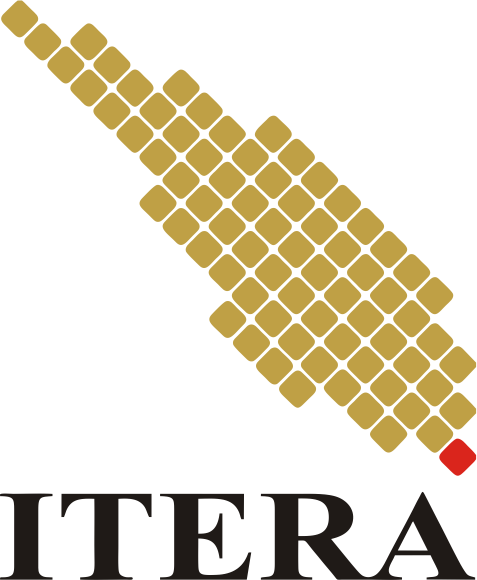
\includegraphics[width=2.1cm, height=2.5cm, keepaspectratio]{figures/itera-logo}
    \end{figure}

	\large \bfseries \MakeUppercase{DETEKSI KANTUK PENGENDARA MOBIL
MENGGUNAKAN \textit{CONVOLUTIONAL NEURAL NETWORKS}}
	\vfill

    \large \uppercase{Tugas Akhir}
    \vfill

    Alfianri Manihuruk\\
    120450088
    \vfill

    \normalsize \bfseries
    \uppercase{
        Program Studi Sains Data \\
        Fakultas Sains\\
        Institut Teknologi Sumatera\\
        Lampung Selatan
    }\medskip

    %\thedate
    % automatic year
    \the\year{}

\end{center}

\clearpage
 % Hardcover
\clearpage
\pagestyle{empty}
\phantomsection% 
\addcontentsline{toc}{chapter}{Halaman Judul}

\begin{center}
\smallskip

    \begin{figure}[h]
    	\centering
    	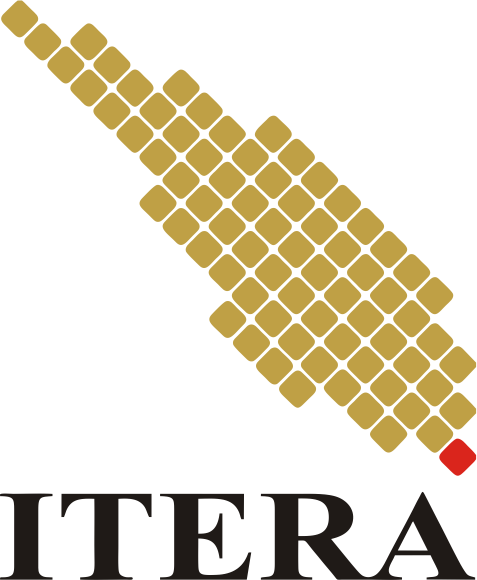
\includegraphics[width=2.1cm, height=2.5cm, keepaspectratio]{figures/itera-logo}
    \end{figure}

	\large \bfseries \MakeUppercase{DETEKSI KANTUK PENGENDARA MOBIL MENGGUNAKAN \textit{CONVOLUTIONAL NEURAL NETWORKS}}
	\vfill

    \large \uppercase{Tugas Akhir}\\
    {\normalsize \normalfont Diajukan sebagai syarat untuk memperoleh gelar sarjana}
    \vfill

    \normalsize \normalfont Alfianri Manihuruk\\
    \ 120450088
    \vfill

    \normalsize \bfseries
    \uppercase{
        Program Studi Sains Data \\
        Fakultas Sains\\
        Institut Teknologi Sumatera\\
        Lampung Selatan
    }\medskip

    %\thedate
    % automatic year
    \the\year{}

\end{center}

\clearpage
 % Softcover
% \clearpage
% \pagestyle{fancy}
% \fancyhf{}
% \fancyhead[R]{\thepage}
% \phantomsection% 
% \addcontentsline{toc}{chapter}{Lembar Pengesahan}

% \begin{center}

% %	\chapter*{\normalsize{Lembar Pengesahan}}
% 	\normalsize \bfseries \MakeUppercase{Lembar Pengesahan} \linebreak
    
%     \normalsize \normalfont \onehalfspacing \justify{
%     Tugas Akhir Sarjana dengan judul \textbf{DETEKSI KANTUK PENGENDARA MOBIL
% MENGGUNAKAN \textit{CONVOLUTIONAL NEURAL NETWORKS}} \ adalah benar dibuat oleh saya sendiri dan belum pernah dibuat dan diserahkan sebelumnya, baik sebagian ataupun seluruhnya, baik oleh saya ataupun orang lain, baik di Institut Teknologi Sumatera maupun di institusi pendidikan lainnya.}

% 	Lampung Selatan, \today{} % TODO: automatic date

% 	\setlength{\tabcolsep}{0pt}
% %	\begin{tabular}{l@{\hskip 0.5in}r}
% 	\begin{tabular}{p{0.7\textwidth}p{0.3\textwidth}}
% 		Penulis, & \multirow{6}{*}{
% 			% Kotak pasfoto 3x4
% 			\begin{tikzpicture}
% 				\draw rectangle (3cm,4cm) node[pos=.5]{
% 					{\begin{tabular}{l}
% 					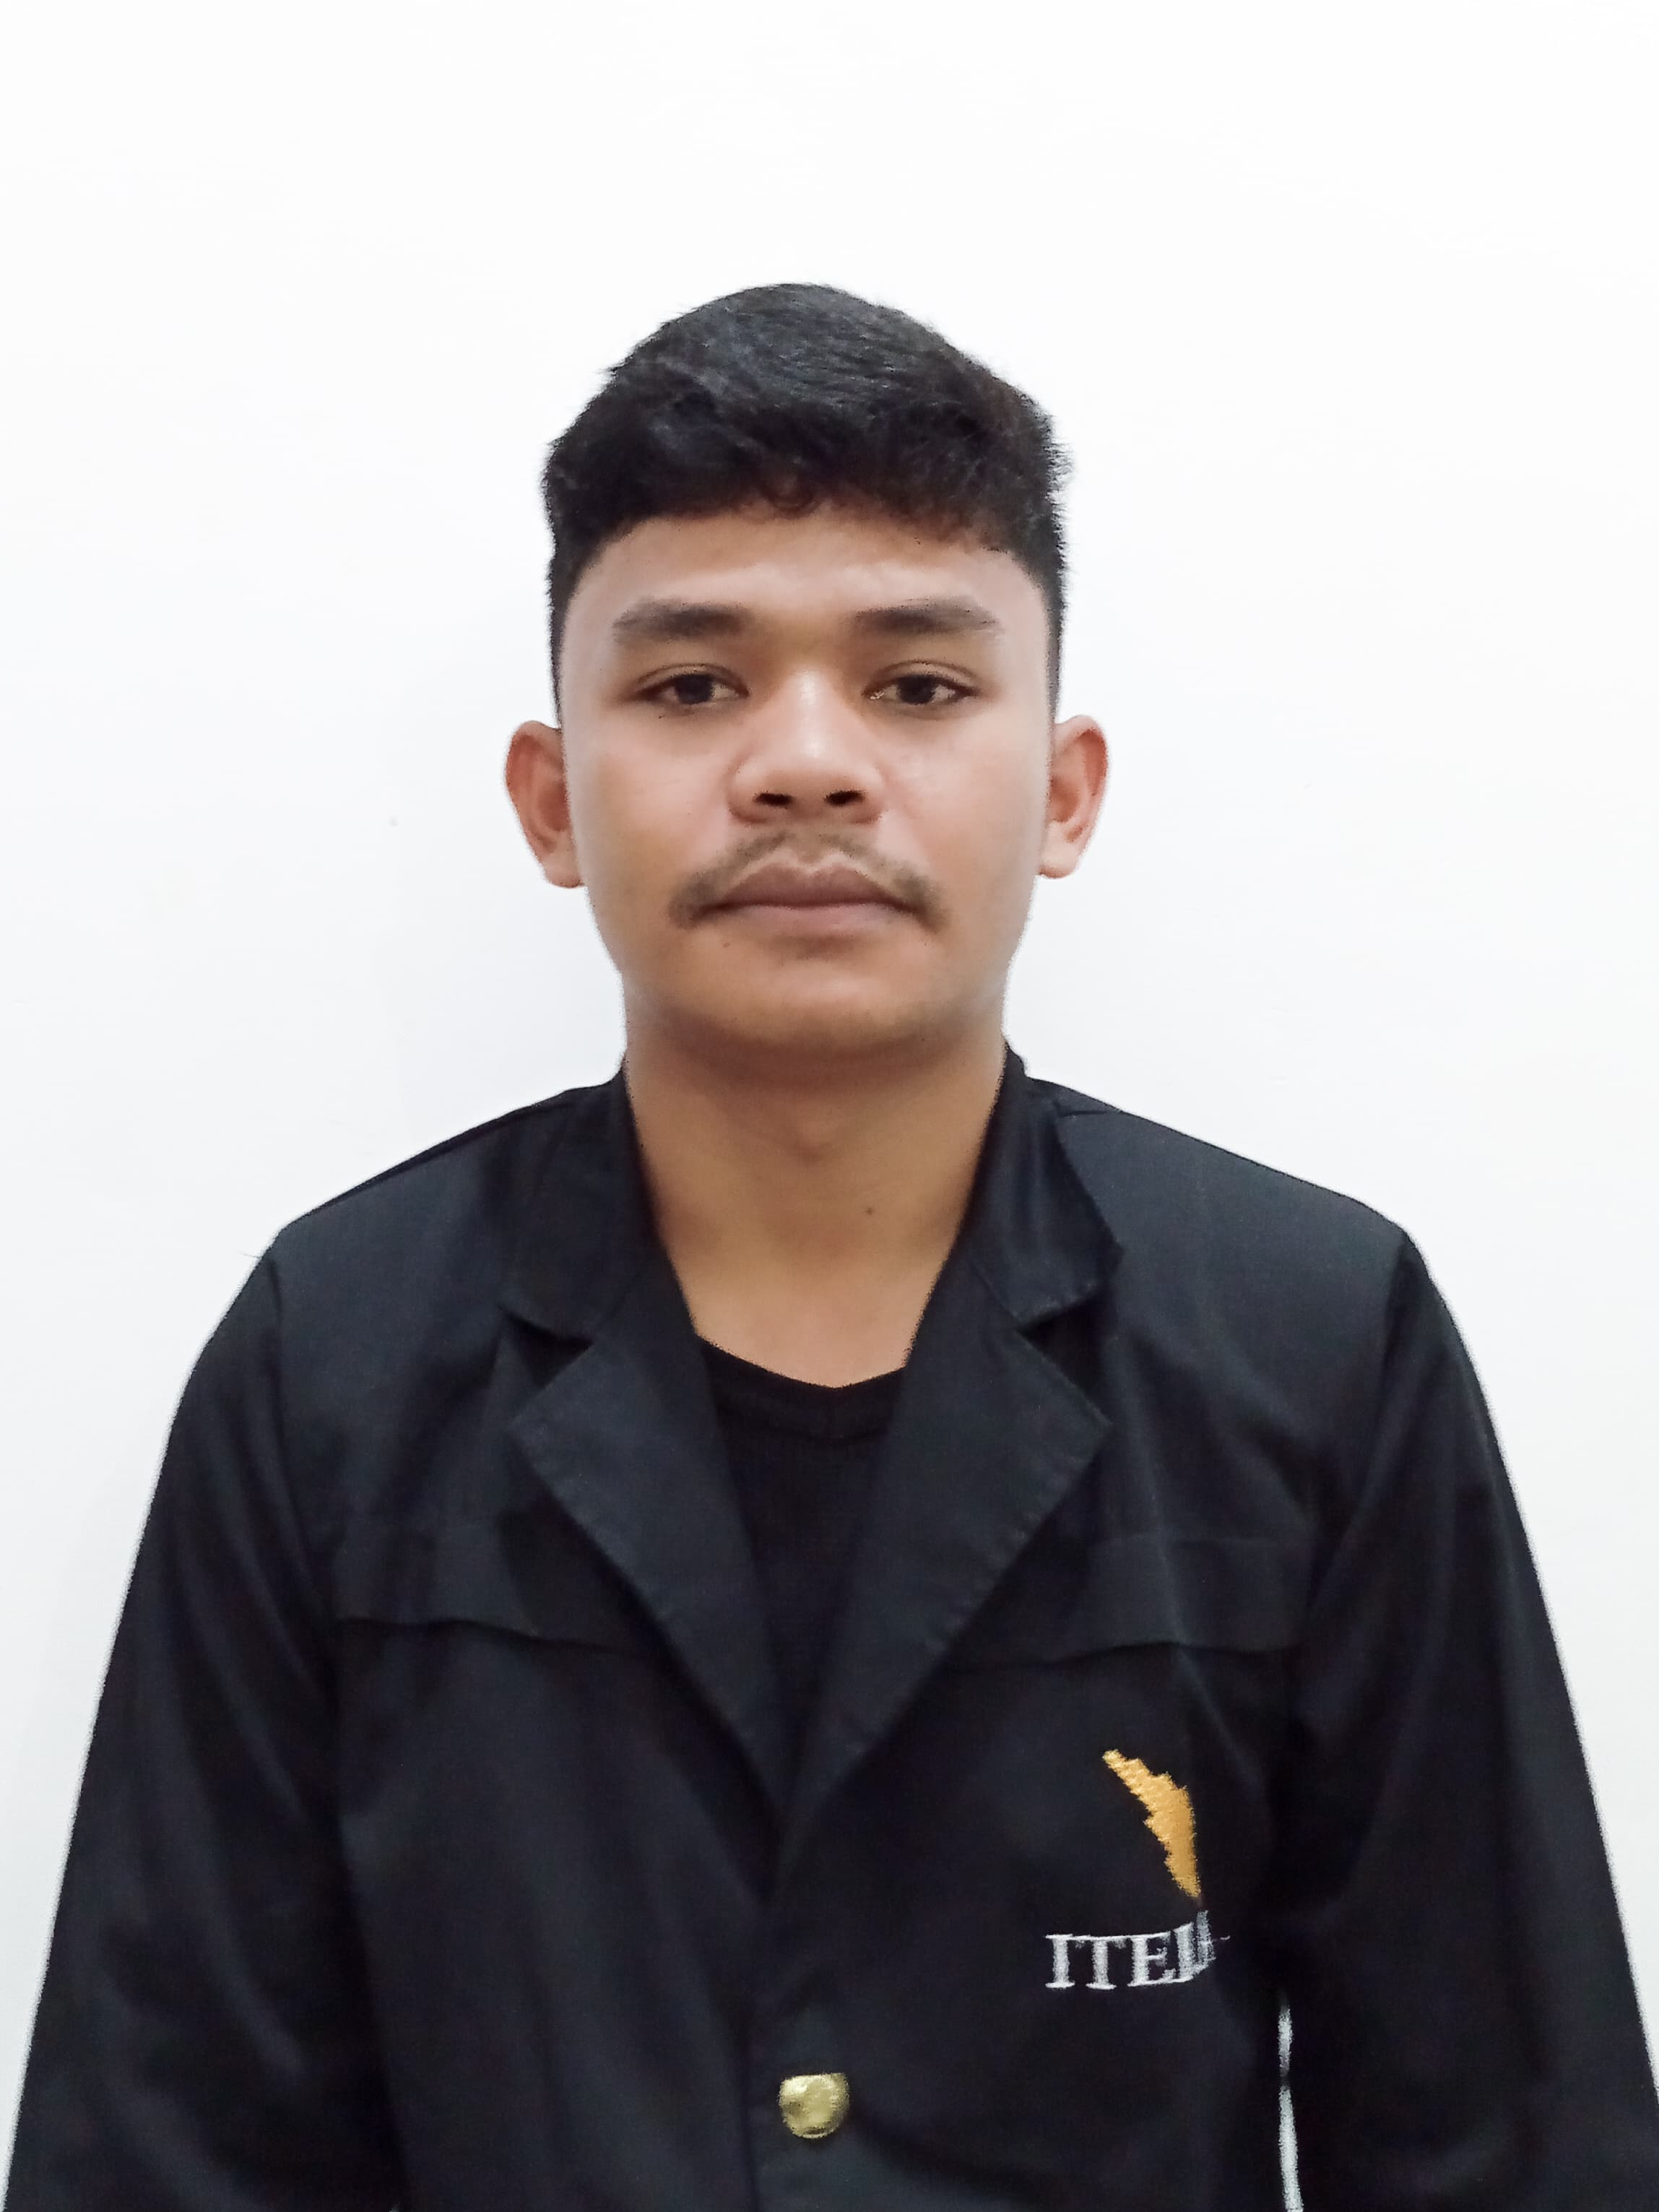
\includegraphics[width=.23\textwidth]{figures/bab0/alfianri.jpeg}
% 					\end{tabular}}};
% 			\end{tikzpicture}
% 			}\\
% 		& \\
% 		& \\
% 		& \\
% 		& \\
% 		Alfianri Manihuruk\\
% 		NIM 120450088
% 	\end{tabular}
% 	\vfill

% 	\centering Diperiksa dan disetujui oleh,
% 	\vspace{2em} % add space
% 	\justify
%     \setlength{\tabcolsep}{0pt}
%     \begin{tabular}{p{0.5\textwidth}p{0.5\textwidth}}
%         \multicolumn{1}{c}{Pembimbing I,} & \multicolumn{1}{c}{Pembimbing II,} \\
%         & \\
%         & \\
%         & \\
%         & \\
% 		\multicolumn{1}{c}{\underline{Tirta Setiawan, S.Pd., M.Si}} & \multicolumn{1}{c}{\underline{Riksa Meidy Karim, S.Kom., M.Si., M.Sc.}} \\
% 		\multicolumn{1}{c}{NIP. 199008222022031003} & \multicolumn{1}{c}{} \\
%     \end{tabular}
% 	\vfill

% 	\centering 
% 	\begin{tabular}{c}
% 		Disahkan oleh,\\
% 		Koordinator Program Studi Sains Data\\
% 		Fakultas Sains\\
% 		Institut Teknologi Sumatera
% 		\\
% 		\\
% 		\\
% 		\\
% 		\\
% 		\underline{Tirta Setiawan, S.Pd., M.Si} \\ % TODO: make automatic
% 		NIP. 199008222022031003 \\
% 	\end{tabular}
	
% \end{center}
% \clearpage



\clearpage
\pagestyle{fancy}
\fancyhf{}
\fancyhead[R]{\thepage}
\phantomsection
\addcontentsline{toc}{chapter}{Lembar Pengesahan}

\begin{center}
	
	\normalsize \bfseries \MakeUppercase{Lembar Pengesahan} \linebreak
	
	\normalsize \normalfont \onehalfspacing \justify{
		Tugas Akhir Sarjana dengan judul \textbf{DETEKSI KANTUK PENGENDARA MOBIL
MENGGUNAKAN \textit{CONVOLUTIONAL NEURAL NETWORKS}} \ adalah benar dibuat oleh saya sendiri dan belum pernah dibuat dan diserahkan sebelumnya, baik sebagian ataupun seluruhnya, baik oleh saya ataupun orang lain, baik di Institut Teknologi Sumatera maupun di institusi pendidikan lainnya.}
	
	\begin{singlespace} \RaggedRight
		Lampung Selatan, \today{} % TODO: automatic date
		\begin{minipage}{0.7\textwidth} % Adjust width as needed
			Penulis, \\[2cm]
			\underline{Alfianari Manihuruk \textcolor{white}{,}} \\
			NIM 120450088 \\[1.5cm]
		\end{minipage}
		\hfill
		\begin{minipage}{0.2\textwidth}
			
\includegraphics[width=\textwidth]{figures/samplephoto.jpg}
		\end{minipage}
		\begin{onehalfspace}
			\\[0.5cm]
		\end{onehalfspace}
	\end{singlespace}	
		\vspace{-0.5cm} % Mengurangi jarak vertikal sebelum subsection
	\centering Diperiksa dan disetujui oleh,
	\vspace{1em} % add space
	\justify
	\setlength{\tabcolsep}{0pt}
	\begin{tabular}{p{0.5\textwidth}p{0.5\textwidth}}
		\multicolumn{1}{c}{Pembimbing I,} & \multicolumn{1}{c}{Pembimbing II,}\\
		&\\
		&\\
		&\\
		\multicolumn{1}{c}{\underline{Tirta Setiawan, S.Pd., M.Si}} & \multicolumn{1}{c}{\underline{Riksa Meidy Karim, S.Kom., M.Si., M.Sc.}} \\
		\multicolumn{1}{c}{NIP. 199008222022031003} & \multicolumn{1}{c}{} \\
	\end{tabular}
	\\
	\centering 
	\begin{singlespace}
		Disahkan oleh,\\
			\vspace{1em} % add space
		Koordinator Program Studi Sains Data\\
		Fakultas Sains\\
		Institut Teknologi Sumatera\\[1.5cm]
		\underline{Tirta Setiawan, S.Pd., M.Si} \\ % TODO: make automatic
		NIP. 19900822 202203 1 003
	\end{singlespace}
\end{center}

	\vspace{0.5cm} % Mengurangi jarak vertikal sebelum subsection
\begin{flushright}
	Sidang Tugas Akhir :     
\end{flushright}
	\vspace{-1.0cm} % Mengurangi jarak vertikal sebelum subsection
%	Penguji  I  : Christyan Tamaro Nadeak, M.Si \\
%	Penguji II : Luluk Muthoharoh, M.Si

	\flushleft
\setlength{\tabcolsep}{0pt}
\begin{tabular}{l l}
	Penguji  I 			&  : Luluk Muthoharoh, M.Si \\
	Penguji  II 		&  : Mika Alvionita S, M.Si
\end{tabular}
\clearpage
\phantomsection% 
\addcontentsline{toc}{chapter}{Halaman Pernyataan Orisinalitas}

\begin{center}
	\smallskip
	
%	\chapter*{\normalsize{Halaman Pernyataan Orisinalitas}}
	\normalsize \bfseries \MakeUppercase{Halaman Pernyataan Orisinalitas} \linebreak
	
	\normalsize \onehalfspacing{
		Tugas Akhir ini adalah karya saya sendiri, dan semua sumber baik yang dikutip maupun dirujuk telah saya nyatakan benar}
	\vspace{3cm}
	
	\centering 
	\begin{tabular}{l l}
		Nama 			& : Alfianri Manihuruk \\
		& \\
		NIM 			& : 12045088 \\
		& \\
		Tanda Tangan 	& : ................................... \\
		& \\
		Tanggal 		& : ................................... \\
	\end{tabular}
	
\end{center}
\clearpage

\clearpage
\phantomsection% 
\addcontentsline{toc}{chapter}{Halaman Persetujuan Publikasi}

\begin{center}
	\smallskip
	
	\normalsize \bfseries \MakeUppercase{
		HALAMAN PERNYATAAN PERSETUJUAN PUBLIKASI \\
		TUGAS AKHIR UNTUK KEPENTINGAN AKADEMIS
	}\linebreak
	
	\normalsize \normalfont \onehalfspacing \justifying{
		Sebagai civitas akademik Institut Teknologi Sumatera, saya yang bertanda tangan di bawah ini:}
	
	\flushleft
	\setlength{\tabcolsep}{0pt}
	\begin{tabular}{l l}
		Nama 			&  : Alfianri Manihuruk\\
		NIM 			&  : 120450088\\
		Program Studi \	&  : Sains Data\\
		Fakultas 		&  : Sains\\
		Jenis Karya 	&  : Tugas Akhir\\
	\end{tabular}

	\justifying
	demi pengembangan ilmu pengetahuan, menyetujui untuk memberikan kepada Institut Teknologi Sumatera \textbf{Hak Bebas Royalti Noneksklusif (Non-exclusive Royalty Free Right)} atas karya ilmiah saya yang berjudul: 
	
	\centering
	\textbf{DETEKSI KANTUK PENGENDARA MOBIL MENGGUNAKAN \textit{CONVOLUTIONAL NEURAL NETWORKS}}
	
	\justifying
	beserta perangkat yang ada (jika diperlukan). Dengan Hak Bebas Royalti Noneksklusif ini Institut Teknologi Sumatera berhak menyimpan, mengalihmedia/formatkan, mengelola dalam bentuk pangkalan data (database), merawat, dan memublikasikan tugas akhir saya selama tetap mencantumkan nama saya sebagai penulis/pencipta dan sebagai pemilik Hak Cipta.
	
	Demikian pernyataan ini saya buat dengan sebenarnya. \\
	
	\centering
	Dibuat di : Lampung Selatan\\
	Pada tanggal : \today{}\\ % Automatic date
	\vspace{3cm}
	Yang menyatakan (Alfianri Manihuruk)
	
	
\end{center}
\clearpage


\clearpage
\centering
\singlespacing{
	\textbf{DETEKSI KANTUK PENGENDARA MOBIL MENGGUNAKAN \textit{CONVOLUTIONAL NEURAL NETWORKS}}\\
 \vspace{1em}
	\mbox{Alfianri Manihuruk (120450088)}\\
 
	\textbf{Pembimbing I Tirta Setiawan, S.Pd., M.Si\\}
	\textbf{Pembimbing II Riksa Meidy Karim, S.Kom., M.Si., M.Sc\\}
}
 \vspace{1em}
%\chapter*{ABSTRAK}
\normalsize \bfseries \centering \MakeUppercase{Abstrak}
\phantomsection% 
\addcontentsline{toc}{chapter}{Abstrak}
\\[2\baselineskip]

%taruh abstrak bahasa indonesia di sini
\justifying \normalfont \normalsize
{

Kecelakaan lalu lintas yang diakibatkan oleh kelalaian manusia, seperti mengantuk saat mengemudi, 
menjadi masalah serius. Karena peristiwa ini  melibatkan kendaraan lain atau pengemudi lain di jalan raya. 
Kelalaian manusia seperti kantuk dapat menyebabkan kecelakaan yang merugikan secara materi dan non materi. 
Banyak pengendara yang mengabaikan rasa kantuk, mereka tetap memaksakan dirinya untuk mengemudi padahal sudah 
seharusnya untuk beristirahat. Penelitian ini mengusulkan deteksi kantuk pengemudi berbasis \textit{Convolutional Neural Network} (CNN) untuk mendeteksi kantuk. Digunakan parameter \textit{Eye Aspect Ratio} (EAR) dan \textit{Mouth Aspect Ratio} (MAR) untuk menentukan kelasya. Terdapat tiga kelas yang dilatih menggunakan CNN untuk mengidentifikasi pola pengendara, seperti 'mengantuk dan menguap', 'mengantuk tidak menguap' dan 'menguap tidak mengantuk'. Ketiga kelas tersebut 
merupakan kombinasi antara parameter EAR \& MAR. Hasil penelitian menunjukkan bahwa model ini mampu mendeteksi kantuk dengan akurasi tinggi. Pada penelitian ini didapatkan hasil terbaik yaitu dengan penggunaan parameter \textit{learning rate} sebesar 0,0001, \textit{activation} ReLU dan \textit{Optimizer} SGD. Dengan performansi model untuk akurasi, \textit{precision}, \textit{recall}, dan \textit{F1-Score} masing-masing 
sebesar 91.76\%, 91.76\%, 92.94\%, dan 91.62\%.

}

\textbf{Kata Kunci}: \textit{Convolutional Neural Network}, \textit{Eye Aspect Ratio}, Kantuk, \textit{Mouth Aspect Ratio}
\clearpage
\clearpage

\begin{minipage}{\textwidth}

\centering
	\singlespacing{
	\textbf{\textit{DRIVER DROWSINESS DETECTION USING
CONVOLUTIONAL NEURAL NETWORKS}}\\
 
 \vspace{1em}
	\mbox{Alfianri Manihuruk (120450088)}\\
	\textbf{Advisor I: Tirta Setiawan, S.Pd., M.Si}\\
	\textbf{Advisor II: Riksa Meidy Karim, S.Kom., M.Si., M.Sc}\\
  
}
\end{minipage}

\vspace{1em}

%\chapter*{ABSTRAK}
\normalsize \bfseries \centering \MakeUppercase{Abstract}
\phantomsection% 
\addcontentsline{toc}{chapter}{Abstract}
\\[2\baselineskip]

%taruh abstrak bahasa inggris di sini
\justifying \normalfont \normalsize

{

\textit{Traffic accidents caused by human negligence, such as drowsiness while driving, are a serious problem because these events involve other vehicles or other drivers on the road. Human negligence such as drowsiness can lead to accidents that have material and non-material costs. Many drivers ignore drowsiness, they still force themselves to drive when they should be resting. This research proposes a driver drowsiness detection system based on Convolutional Neural Network (CNN) to detect drowsiness. The parameters of Eye Aspect Ratio (EAR) and Mouth Aspect Ratio (MAR) are used to determine the class. There are three classes trained using CNN to identify driver patterns, such as 'sleepy and yawning', 'sleepy not yawning' and 'yawning not sleepy'. The three classes 
are a combination of EAR \& MAR parameters. The results show that this system is able to detect drowsiness with high accuracy. In this study, the best results were obtained by using the parameters \textit{learning rate} 0.0001, \textit{activation} ReLu and \textit{Optimizer} SGD. With system performance for accuracy, precision, recall, and F1-Score of respectively 92.97\%, 93.32\%, 92.72\%, and 92.98\%, respectively.
}

}

\textbf{Keyword}: \textit{Convolutional Neural Network, Drowsiness, Eye Aspect Ratio, Mouth
Aspect Ratio}

\clearpage
\clearpage

\normalsize \bfseries \centering \MakeUppercase{Motto}
\phantomsection% 
\addcontentsline{toc}{chapter}{Motto}
\\[2\baselineskip]

\justifying \normalfont{

\centering\textbf{"TIDAK ADA ALASAN UNTUK TIDAK BERSYUKUR"}\vspace{1em}



\centering"Direndahkan dimata manusia, ditinggikan dimata Tuhan, \textit{Prove that you are better than you were before"}\vspace{1em}


\centering"Aku ditolak dengan hebat sampai jatuh, tetapi Tuhan menolong aku"\\
(Mazmur 118:13)\vspace{1em}


\centering"Aku tahu, bahwa Engkau sanggup melakukan segala sesuatu dan tidak ada rencana-Mu yang gagal"\\
(Ayub 42:2)\vspace{1em}


\centering“Pencobaan-pencobaan yang kamu alami ialah pencobaan-pencobaan biasa, yang tidak melebihi kekuatan manusia. Sebab Allah setia dan karena itu Ia tidak akan membiarkan kamu dicobai melampaui kekuatanmu"\\

(1 Korintus 10 : 13)\vspace{1em}


\centering"Jangan takut, percaya saja"\\
(Markus 5:36)\vspace{1em}

\centering"Karena masa depan sungguh ada dan harapan-Mu tidak akan hilang"\\
(Amsal 23:18)\vspace{1em}

	% Motto

}

\clearpage
\clearpage

% PS: Ada bug dimana jika menge-build dari file ini, ada error. Tapi halamannya
% sendiri tidak error jika dibuild dari file lain. (Radhinka)

\normalsize \bfseries \centering \MakeUppercase{Persembahan}
\phantomsection% 
\addcontentsline{toc}{chapter}{Persembahan}
\\[2\baselineskip]

\justifying \normalfont{
	% Kata-kata persembahan
Dengan rendah hati dan penuh rasa syukur, karya ini saya dedikasikan untuk kedua orang tua yang tiada hentinya memberikan kebaikan yang tak terhingga kepada anak-anaknya. Terima kasih kepada setiap individu baik yang telah melintasi hidup saya, mewarnainya dengan cerita indah, meskipun tak dapat saya sebutkan satu per satu. Dan tak lupa, penghargaan yang mendalam saya tujukan untuk almamater tercinta, Institut Teknologi Sumatera, tempat di mana perjalanan ilmu dan kehidupan tak terlupakan dimulai. Semoga karya ini dapat menjadi cerminan kebaikan dan kasih sayang yang selalu mengalir dari hati kita
}

\clearpage
\clearpage

\normalsize \bfseries \centering \MakeUppercase{Kata Pengantar}
\phantomsection% 
\addcontentsline{toc}{chapter}{Kata Pengantar}
\thispagestyle{fancy}
\fancyhf{}
\fancyhead[R]{\thepage}
\\[2\baselineskip]

\normalsize \normalfont \justifying
    Puji dan Syukur kepada Tuhan Yang Maha Esa, atas segala pertolongan dan rahmatNya sehingga penulis dapat menyelesaikan tugas akhir yang berjudul ”DETEKSI KANTUK PENGENDARA MOBIL MENGGUNAKAN\textit{ CONVOLUTIONAL NEURAL NETWORKS}”.
    Penyusunan tugas akhir ini dilakukan dengan penuh dedikasi dan semangat. Oleh
    karena itu, dengan senang hati penulis menyampaikan laporan penelitian ini sebagai syarat untuk memperoleh gelar sarjana Program Studi Sains Data, Fakultas
    Sains, Institut Teknologi Sumatera (ITERA). Terima kasih penulis sampaikan kepada semua pihak yang telah membantu dan mendukung selama proses penelitian
    ini, ditujukan kepada:

        \begin{itemize}
        
        \item Bapak Tirta Setiawan, S.Pd, M.Si. selaku dosen pembimbing utama dan koordinator program studi sains data.
        
        \item Bapak Riksa Meidy Karim, S.Kom., M.Si., M.Sc beserta Ibu Amalya Citra S.Kom., M.Si., M.Sc, selaku dosen pembimbing pendamping yang telah memberikan arahan, ilmu, motivasi, serta saran kepada penulis selama proses penyusunan Tugas Akhir.
        
        \item Dosen dan staff pengajar program studi sains data yang telah membantu dalam penulisan tugas akhir saya.
        
        \item Kedua orang tua dan keluarga saya yang selalu mendukung dan mendoakan saya selama masa pekuliahan dan masa penulisan Tugas Akhir (TA).

        \item Hotbin Manihuruk beserta keluarga yang telah menjadi tempat saya berkeluh kesah dan belajar banyak terkait kehidupan.
        
        \item Teman-teman satu kontrakan saya Donni Marulitua Taringan dan Rendi Hasiholan Manullang yang telah menjadi keluarga satu rumah.
        Demikian kata pengantar ini, semoga laporan ini memberikan kebermanfaatan.

        \item Dimas dan teman-teman satu bimbingan yang telah menjadi kelompok bimbingan yang saling mengingatkan.
        Demikian kata pengantar ini, semoga laporan ini memberikan kebermanfaatan.
        
        \end{itemize}

\flushright{
	Lampung Selatan, 15-Februari-2024\\
	Penulis,
	\\[5\baselineskip]
	Alfianri Manihuruk
}

\clearpage


\tableofcontents
\listoffigures
\listoftables


    %----------------------------------------------------------------%
    % Konfigurasi Bab
    %----------------------------------------------------------------%
    \renewcommand{\chaptername}{BAB}
    % Bab: Arabic
    \renewcommand{\thechapter}{\Roman{chapter}}
    % Sub-bab: Roman
    \renewcommand\thesection{\arabic{chapter}.\arabic{section}}
    
    % Setting supaya nomor halaman pertama dengan "chapter"
    % berada di tengah bawah
    \fancypagestyle{plain}{%
    	\fancyhf{}%
    	\renewcommand{\headrulewidth}{0pt}
    	\fancyhead[]{}
    	\fancyfoot[C]{\thepage}
    }
    %----------------------------------------------------------------%

    %----------------------------------------------------------------%
    % Daftar Bab
    % Untuk menambahkan daftar bab, buat berkas bab misalnya `chapter-6` di direktori `chapters`, dan masukkan ke sini.
    %----------------------------------------------------------------%

    % Reset penomoran halaman menjadi 1
    \clearpage
    \setcounter{page}{1}
    \pagenumbering{arabic}

    \justifying
    \chapter{PENDAHULUAN}
\pagestyle{plain}
\section{Latar Belakang}

    Kecelakaan lalu lintas merupakan masalah serius yang dihadapi masyarakat, karena peristiwa ini tidak terduga dan melibatkan kendaraan lain atau pengemudi lain di jalan raya \cite{himawan2022deteksi}. Organisasi Kesehatan Dunia (WHO) mencatat bahwa pada tahun 2019, kecelakaan di jalan raya telah menyebabkan kehilangan nyawa sebanyak 1,35 juta orang di seluruh dunia, 20\%-30\% disebabkan karena kelalaian manusia \cite{kojo2024analisis}. Kelalaian manusia seperti kantuk dapat menyebabkan kecelakaan yang merugikan secara materi dan non materi. Banyak pengendara yang mengabaikan rasa kantuk, mereka tetap memaksakan dirinya untuk mengemudi padahal sudah seharusnya untuk beristirahat   \cite{Puteri2020}.

    Kantuk merupakan kondisi alami yang dialami oleh manusia seperti waktu reaksi yang lebih lambat. Kantuk dapat menyebabkan penurunan respons dan kinerja tubuh \cite{Chaabene2021}. Keadaan mengantuk sangat berbahaya, terutama pada saat berkendara. Pengemudi yang mengantuk memiliki waktu reaksi yang lama dan tidak dapat membuat keputusan dengan cepat, sehingga dapat menyebabkan kecelakaan lalu lintas \cite{Cui2021}. Mengemudi dalam keadaan mengantuk merupakan sebuah tindakan yang sangat berbahaya karena dapat mengancam keselamatan banyak orang \cite{Ngxande2017}. Masalah utama bagi pengemudi yaitu, ketika mereka tidak dapat mengetahui tingkat dimana mereka harus berhenti untuk mengemudi dengan aman. Untuk mengatasi masalah tersebut dapat diminimalisir dengan melakukan deteksi kantuk pada pengemudi, serta memberikan peringatan apabila pengemudi mengantuk \cite{Zhu2022}. 

    Kantuk yang menyebabkan kecelakaan dapat dicegah dengan bantuan sistem deteksi kantuk pada pengemudi. Sistem memantau pengemudi dan memberikan pering-atan untuk meminta pengemudi menghentikan kendaraan selama pengemudi mengantuk \cite{Cui2021}. Deteksi keadaan mengantuk pada pengemudi di implementasikan dengan menggunakan kamera dan pengolahan citra digital. Keadaan mata (terbuka atau tertutup) menjadi parameter dalam menentukan pengendara mengantuk \cite{sethu2023application}. Kamera akan mengambil gambar kemudian ditentukan apakah objek yang diamati sedang dalam keadaan mengantuk atau tidak. Pada saat pengendara terdeteksi sedang mengantuk, sistem dengan segera akan memberikan peringatan agar pengemudi dapat beristirahat dan melakukan pergantian sopir. Untuk menciptakan sistem seperti itu, dapat digunakan metode \textit{deep learning} dan kombinasi pemrosesan dan pengenalan pola dalam gambar digital \cite{Imanuddin2019}.

    \textit{Deep learning} telah berkembang pesat dan tak lagi terbatas pada pengenalan gambar. Saat ini, \textit{deep learning} diaplikasikan untuk berbagai macam permasalahan, termasuk klasifikasi. \textit{Convolutional Neural Network} (CNN) digunakan untuk mengidentifikasi pola citra pengendara kantuk pada saat berkendara. 
    Setelah kepopuleran \textit{deep learning} meningkat pasca kemunculan \textit{AlexNet}, variasi arsitektur \textit{Convolutional Neural Network} (CNN) berhasil memenangkan \textit{ImageNet Large Scale Visual Recognition Challenge} (ILSVRC) pada tahun 2012. AlexNet merupakan arsitektur \textit{Convolutional Neural Network} (CNN) yang memainkan peran penting dalam perkembangan \textit{deep learning}, khususnya dalam pengolahan gambar. Diperkenalkan pada tahun 2012 oleh Alex Krizhevsky, Ilya Sutskever, dan Geoffrey Hinton. 
    
    
    \textit{Convolutional Neural Network} (CNN) telah menjadi metode yang banyak diguna-kan di berbagai bidang, termasuk pertanian dan perkebunan. Sebagai contoh, dalam penelitian yang dilakukan oleh Mauricio Rodriguez dkk, metode CNN digunakan untuk mengklasifikasikan tingkat kematangan lima jenis buah. Hasil yang diperoleh menunjukkan bahwa model terbaik, dengan akurasi 96,34\%, telah berhasil mengidentifikasi kualitas kematangan dari lima buah tersebut \cite{Rodriguez2021}. Penelitian yang dilakukan Cahya Aji Saputra menggunakan metode CNN untuk mendeteksi rasa kantuk pada pengemudi. Perangkat mengenali mata terbuka dan tertutup. Akurasi 95,4\% pada jarak 30 hingga 50 cm dan akurasi waktu nyata sebesar 93,9\%, metode ini berpotensi untuk mengurangi kemungkinan terjadinya kecelakaan akibat rasa kantuk yang tidak diperoleh pengemudi \cite{Saputra2021}.

    Dengan menerapkan metode \textit{Convolutional Neural Network} (CNN), dalam studi ini akan dilakukan deteksi keadaan pengendara dengan mengidentifikasi tanda-tanda kantuk pada pengemudi melalui analisis citra dari kondisi mata dan mulut. Penentuan kondisi mata dan mulut dilakukan dengan menghitung nilai 
    \textit{Eye Aspect Ratio} (EAR) dan \textit{Mouth Aspect Ratio} (MAR). Data yang dihasilkan berdasarkan kondisi tersebut akan dilakukan klasifikasi menggunakan \textit{Convolutional Neural Network} (CNN). Hasil penelitian ini diharapkan dapat mendeteksi kondisi pengendara yang mengantuk.

   
\section{Rumusan Masalah}
Rumusan masalah dalam penelitian ini adalah berikut:
\begin{enumerate}

    \item Bagaimana penerapan \textit{Convolution Neural Network} (CNN) dalam mendeteksi kantuk berdasarkan kondisi mata dan mulut?

    \item Berapa dan bagaimana pengaruh parameter \textit{Convolution Neural Network} (CNN) yang optimal untuk meningkatkan performa klasifikasi kantuk?
\end{enumerate}


\section{Tujuan}
Tujuan dari penelitian ini adalah sebagai berikut.

\begin{enumerate}

    \item Melakukan deteksi kantuk pada pengendara dengan metode \textit{Convolutional Neural Network} (CNN) berdasarkan kondisi mata dan mulut.
    
    \item Menganalisis pengaruh parameter CNN terhadap performa klasifikasi kantuk.

\end{enumerate}
\section{Batasan Masalah}
Batasan permasalahan pada penelitian ini adalah sebagai berikut:
\begin{enumerate}

    \item Data yang digunakan merupakan data berupa video pengendara 
    yang berasal dari YAWDD: YAWNING DETECTION DATASET. dengan hanya
    mengambil data "yawning" dan "talking \& yawning"
    \item Penelitian ini akan berfokus pada kondisi mata dan mulut untuk deteksi keadaan pengendara. Aspek lain seperti deteksi wajah tidak akan dibahas secara rinci. 
    \item Parameter CNN yang digunakan adalah \textit{activation layer}, \textit{learning rate} dan \textit{optimazer}
    \item Pembuatan model terbatas hanya untuk klasifikasi kantuk pada tiga kelas yaitu: “mengantuk dan menguap”, “mengantuk tidak menguap” dan “menguap tidak mengantuk”

    

\end{enumerate}
    \chapter{LANDASAN TEORI}

\section{Tinjauan Pustaka}


    Dalam penelitian ini, beberapa teori dasar 
    akan digunakan untuk memberikan penjelasan 
     lebih komprehensif terhadap proses penelitian 
     dan mendalami pemahaman terkait dengan topik 
     yang diadopsi. Untuk mendukung metodologi 
     penelitian ini, beberapa sumber referensi 
     akan digunakan sebagai acuan untuk mengkaji 
      konsep dasar pengolahan citra digital, 
      pengenalan gambar dalam bentuk objek digital, 
      serta metode yang digunakan. Metode penelitian 
       dipilih yaitu \textit{Convolutional Neural Network}  (CNN) akan 
       dijelaskan secara rinci pada bagian selanjutnya. Metode CNN 
       digunakan dikarena pendekatan ini merupakan jenis 
       teknik \textit{neural network} yang secara khusus dibuat 
       untuk mengatasi masalah pada data dua dimensi (2D) yang terdiri 
       dari berbagai ukuran piksel \cite{Lindholm2022}. Beberapa 
       mengenai deteksi kantuk dapat dilihat pada Tabel \ref{Tabel Perbandingan Referensi} berikut.

    

      \begin{table}[H]
        \centering
        \caption{Penelitian Mengenai Deteksi Kantuk}
         \label{Tabel Perbandingan Referensi}
        \begin{tabular}%{p{0.5cm}p{1.8cm}p{2.9cm}p{1.1cm}p{4.1cm}p{1cm}}
              {  >{\raggedright\arraybackslash}p{0.3cm} 
        >{\raggedright\arraybackslash}p{2.0cm} 
        >{\raggedright\arraybackslash}p{2.5cm} 
        >{\raggedright\arraybackslash}p{1.5cm} 
        >{\raggedright\arraybackslash}p{4.0cm} 
        >{\raggedright\arraybackslash}p{0.9cm}}
    
            \hline
            \textbf{No} & \textbf{Penulis} & \textbf{Topik} &\textbf{ Metode} & \textbf{Hasil} & \textbf{Tahun} \\
            
            \hline
             1 
            & 
            Fiaz Majeed, Umair Shafique, Mejdl Safran, Sultan Alfarhood, and Imran Ashraf
            &
            \textit{Detection of Drowsiness among Drivers Using Novel Deep Convolutional Neural Network Model}
            & 
            CNN \& RNN
            &
            Hasil eksperimen menunjukkan bahwa model yang diusulkan mencapai akurasi rata-rata 96,69\% tanpa augmentasi data, yang lebih unggul dari yang sudah ada yang sudah ada dalam mendeteksi kantuk 
            &
            2023 \\  
            \\

             2 
            & 
            Ruben Florez, Facundo Palomino-Quispe, Roger Jesus Coaquira-Castillo, Julio Cesar, Thuanne and Ana Beatriz
            & 
            \textit{A CNN-Based Approach for Driver Drowsiness Detection by Real-Time Eye State Identification}
            & 
            CNN
            &
            Dari 10 percobaan yang dilakukan dan menunjukkan hasil akurasi yang tinggi dalam mendeteksi kantuk menggunakan CNN berdasaran tiga arsitektur  yaitu InceptionV3, VGG16 dan ResNet50V2. Dengan akurasi masing-masing sebesar 99.31\%, 99.41 \%, dan 99.71\%. 
            &
            2023 \\
                \hline

        \end{tabular}
    \end{table}




         \begin{table}[H]
        \centering
        \begin{tabular}%{p{0.5cm}p{1.8cm}p{2.9cm}p{1.1cm}p{4.1cm}p{1cm}}
        {>{\raggedright\arraybackslash}p{0.3cm} 
        >{\raggedright\arraybackslash}p{2.0cm} 
        >{\raggedright\arraybackslash}p{2.5cm} 
        >{\raggedright\arraybackslash}p{1.5cm} 
        >{\raggedright\arraybackslash}p{4.0cm} 
        >{\raggedright\arraybackslash}p{0.9cm}}
    
            \hline
            \textbf{No} & \textbf{Penulis} & \textbf{Topik} &\textbf{ Metode} & \textbf{Hasil} & \textbf{Tahun} \\    
            \hline

            3 
            & 
            Hepatika Zidny Ilmadina, Dyah Apriliani, Dega Surono Wibowo
            &
            Deteksi Pengendara Mengantuk dengan Kombinasi Haar 
                \textit{Cascade Classifier} dan \textit{Support Vector Machine}
            &
            SVM \& KNN
            &
            Berdasarkan percobaan yang telah dilakukan diperoleh evaluasi untuk SVM untuk \textit{accuracy} 0.99, \textit{precision} 0.99, dan recall 0.99 dan untuk KNN \textit{accuracy} 0.97, \textit{precision} 0.89, dan \textit{recall} 0.99. Berdasarkan data tersebut dapat disimpulkan bahwa performa yang baik dicapai oleh model SVM dibandingkan dengan KNN.
            &
            2020 \\
            \\
        
                4
            &
            Venkata Rami Reddy Chirra1, Srinivasulu Reddy, Venkata Krishna Kishore
            &
            \textit{Deep CNN: A Machine Learning Approach for Driver Drowsiness Detection Based on Eye State}
            &
            CNN
            &
            Dari 1200 sampel latih, 1150 sampel uji dan 500 sampel validasi, diperoleh  akurasi latih sebesar 98\%. Akurasi validasi 97\% dan akurasi uji 96.42\%

            &

            2019 \\
            \\

             5
            & 
            Tereza Soukupova and Jan ´Cech &
           \textit{ Real-Time Eye Blink Detection using Facial Landmarks} &
            EAR SVM &

           Pada deteksi \textit{landmarks} kesalahan cukup kecil hingga 5\% dari IOD tetapi untuk \textit{interface} kesalahan di bawah 10\%. Pada deteksi kedipan akurasi tetap tinggi hingga rata-rata IOD sekitar 30 px.
             &
            2017\\

             \hline

        \end{tabular}
    \end{table}



        


       
\section{Kecelakaan}

    Menurut Undang-Undang (UU) Republik Indonesia Pasal 1 No. 22 tahun 2009, kecelakaan lalu lintas dapat diartikan sebagai peristiwa yang terjadi di jalan raya secara tiba-tiba dan tidak disengaja, melibatkan kendaraan atau pengguna jalan lainnya, dan berakibat pada korban jiwa atau kerusakan harta benda. Kondisi kantuk dapat menjadi salah satu faktor yang menyebabkan kecelakaan lalu lintas. Kantuk dapat mengurangi kewaspadaan dan reaksi pengemudi, sehingga meningkatkan risiko terjadinya kecelakaan. Selain itu, kelelahan juga dapat menjadi penyebab utama terjadinya kantuk saat berkendara. Faktor-faktor lain yang dapat menyebabkan kecelakaan lalu lintas meliputi kelalaian pengguna jalan, kondisi kendaraan yang tidak layak jalan, kondisi jalan yang tidak memadai, serta kondisi lingkungan seperti cuaca buruk atau jalan yang licin \cite{Utomo2023}.
    

\section{Kantuk}
    Kantuk merupakan keadaan di mana seseorang merasa ingin tidur. Biasanya,
     kondisi ini disertai dengan mata yang terasa berat dan sulit 
     berkonsentrasi. Kantuk seringkali ditandai dengan keadaan menguap. 
     Ini adalah respons fisiologis yang umum terjadi pada manusia. 
     Ketika seseorang merasa kantuk, otak dapat mengirim sinyal 
     untuk mengurangi kejernihan dan kewaspadaan. Salah satu tanda-tanda 
     menguap sering kali disertai dengan membuka mulut lebar \cite{CALDWELL2019272}. Kantuk merupakan gejala dari kelelahan yang dipengaruhi oleh waktu dan mekanisme homeostasis dalam tubuh.
     
    Homeostasis adalah mekanisme yang menjaga keseimbangan internal tubuh, termasuk dalam hal tidur dan bangun. Keadaan ini biasanya terjadi pada malam hari saat tubuh secara alami merasa lebih siap untuk tidur, namun juga dapat terjadi pada siang hari akibat kurangnya tidur atau perubahan jam tidur yang eksternal. Meskipun kantuk pada siang hari dianggap wajar, tetapi dapat menjadi masalah jika terjadi saat berkendara atau melakukan aktivitas lain yang memerlukan kewaspadaan \cite{Puspasari2023}.
    Rasa kantuk dapat mengakibatkan berbagai masalah, termasuk menghambat 
    produktivitas di tempat kerja, memengaruhi emosi, dan menyebabkan 
    kecelakaan, baik di jalan maupun di tempat kerja. Meskipun rasa 
    mengantuk adalah hal yang biasa, jika terjadi secara tidak normal, 
    hal ini mungkin mengindikasikan gejala penyakit. Seperti sleep apnea, 
    narkolepsi, insomnia, depresi, gangguan kecemasan, atau 
    diabetes \cite{Susanto2020}.

    Akibat merasakan kantuk, seseorang bisa mengalami \textit{microsleep}, yaitu keadaan hilang kesadaran. Peristiwa ini biasanya terjadi selama 1 detik hingga 2 menit. \textit{Microsleep} terjadi karena aktivitas yang monoton, seperti menatap layar komputer terus menerus atau berkendara dalam waktu yang cukup lama. Teori ini digunakan sebagai acuan untuk mendeteksi kondisi kantuk berdasarkan kondisi mata. Apabila mata tertutup kurang dari 3 detik, berarti keadaan tidak mengantuk. Namun, jika mata tertutup lebih dari 3 detik, pengendara sedang mengantuk \cite{puteri2020deteksi}.

\section{\textit{Computer Vision}}

    \textit{Computer Vision} adalah bidang dalam ilmu komputer yang berkonsentrasi pada pembuatan algoritma untuk memberdayakan komputer dalam memahami gambar dan video \cite{Guntara2023}. \textit{Computer Vision }telah berkembang di berbagai domain, mencakup kegiatan seperti menangkap data mentah dan mengekstraksi pola dari gambar untuk menginterpretasikan informasi. \textit{Computer Vision} menggabungkan berbagai metode, prinsip, dan konsep yang berasal dari pemrosesan citra digital, pengenalan pola, kecerdasan buatan, dan grafik komputer. Mayoritas tugas dalam \textit{computer vision} berkisar pada perolehan informasi tentang suatu peristiwa atau deskripsi dari masukan gambar digital, termasuk ekstraksi fitur \cite{Noerifanza2022}. 


    \textit{Computer Vision} diidentifikasi sebagai disiplin ilmu dengan seperangkat teknik yang bertujuan untuk memungkinkan komputer memahami konten gambar digital. Bidang multidisiplin ini sebagian besar dibangun di atas konsep pembelajaran mesin, yang menggabungkan algoritma pembelajaran yang terus berkembang. Tujuan utamanya adalah mengembangkan sistem otomatis yang mampu mengekstraksi informasi dari gambar digital yang diberikan.  Deskripsi mengenai \textit{computer vision}, seperti yang diilustrasikan pada Gambar \ref{Konsep Dasar Computer Vision} \cite{Guntara2023} berikut.


    \begin{figure}[H]
        \centering
        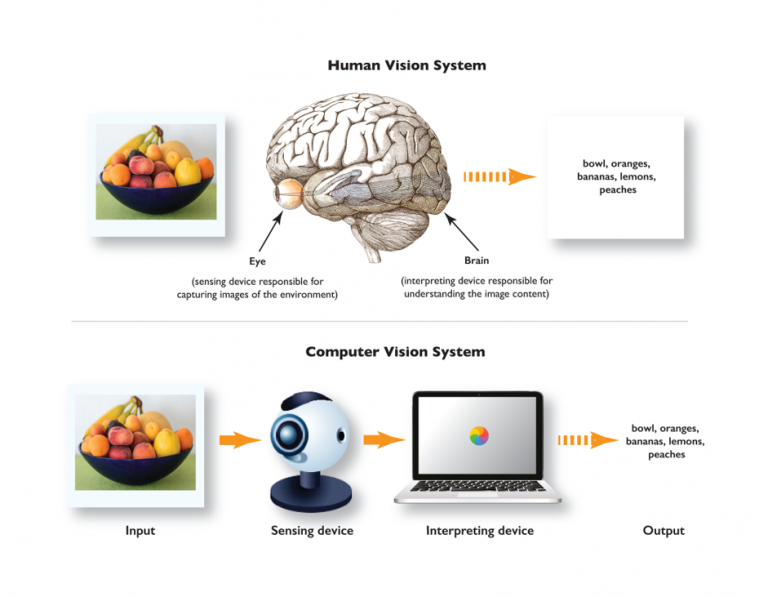
\includegraphics[width=0.7\textwidth]{figures/bab2/computer vision.jpg}
        \caption{Ilustrasi \textit{Computer Vision} \cite{ideas}}
        \label{Konsep Dasar Computer Vision}
    \end{figure}


   


\section{Pengolahan Citra Digital}

    Pemrosesan gambar digital dibagi menjadi tiga tingkatan yang berbeda sebagai berikut: 

    \begin{enumerate}
    
        \item  Tingkat rendah, melibatkan operasi mendasar pada gambar digital, termasuk tugas-tugas seperti akuisisi gambar, dan merekayasa kualitas gambar. Hal ini dicapai melalui tindakan seperti peningkatan kontras, pengurangan atau penambahan \textit{noise}, dan penajaman gambar.

        \item  Tingkat menengah, pemrosesan komputer mencakup operasi yang lebih rumit dalam menangani gambar, khususnya mengubah ukuran, memotong, dan segmentasi. Tingkat pemrosesan ini memiliki hasil yang berbeda dari proses tingkat yang lebih rendah, karena proses ini mengambil data gambar sebagai masukan dan menghasilkan informasi berbeda yang telah diekstraksi secara efektif dari gambar. Informasi yang diekstraksi ini mungkin mencakup fitur seperti kontur, deteksi tepi, dan detail relevan lainnya.

        \item Tingkat tinggi, di mana pemrosesan gambar diarahkan untuk mengidentifikasi objek dalam gambar yang diberikan. Tahap ini  melibatkan pembelajaran mesin, klasifikasi, dan berbagai algoritma kecerdasan buatan.

    \end{enumerate}
    
    
    
  Untuk pemahaman yang lebih mendalam mengenai perkembangan pada setiap tahap pemrosesan gambar digital, berikut representasi visual yang ditunjukkan pada Gambar \ref{Proses Dalam Pengolahan Citra Digital} berikut ini.


    \begin{figure}[H]
    \centering
    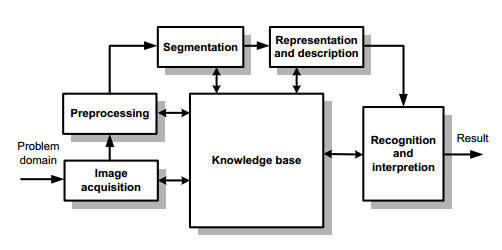
\includegraphics[width=0.75\textwidth]{figures/bab2/Block-diagram.jpg}
    \caption{Proses Pengolahan Citra Digital \cite{sathiya2017novel}}
    \label{Proses Dalam Pengolahan Citra Digital}
\end{figure}

    

    Tujuan pemrosesan gambar digital adalah menghasilkan gambar berkualitas tinggi, memfasilitasi ekstraksi informasi yang mudah, baik oleh manusia maupun mesin.
    Teknik dalam pengolahan citra juga dapat digunakan untuk mentrasformasikan citra digital menjadi sebuah citra lain \cite{Kirana2021}.  

\subsection{Citra Digital}

    Citra digital merupakan representasi gambar dua dimensi menggunakan satu set nilai digital tertentu, yang sering disebut sebagai piksel atau elemen gambar. Citra terdiri dari $m \times n$ piksel, di mana setiap piksel diwakili oleh $k$ bit. Sebuah piksel, dilambangkan dengan $k$-bit, memiliki $2^k$ corak berbeda dalam gambar skala abu-abu. Nilai piksel ini biasanya terdiri dari bilangan bulat dalam rentang 0 (mewakili piksel hitam) hingga $(2^k - 1)$ (mewakili piksel putih). Besaran nilai piksel ini memainkan peran penting dalam menentukan resolusi dan mempengaruhi kualitas gambar secara keseluruhan \cite{book}. Nilai yang menentukan intensitas gambar atau derajat skala abu-abu atau warna dalam suatu gambar dinyatakan sebagai fungsi dari intensitas gambar, dilambangkan dengan $f(x, y)$. Hal ini muncul dari representasi suatu gambar sebagai matriks dua dimensi, seperti yang digambarkan pada Gambar \ref{Sistem Koordinat Matematis Sebuah Citra} \cite{Andono2018} berikut.

    \begin{figure}[H]
      \centering
      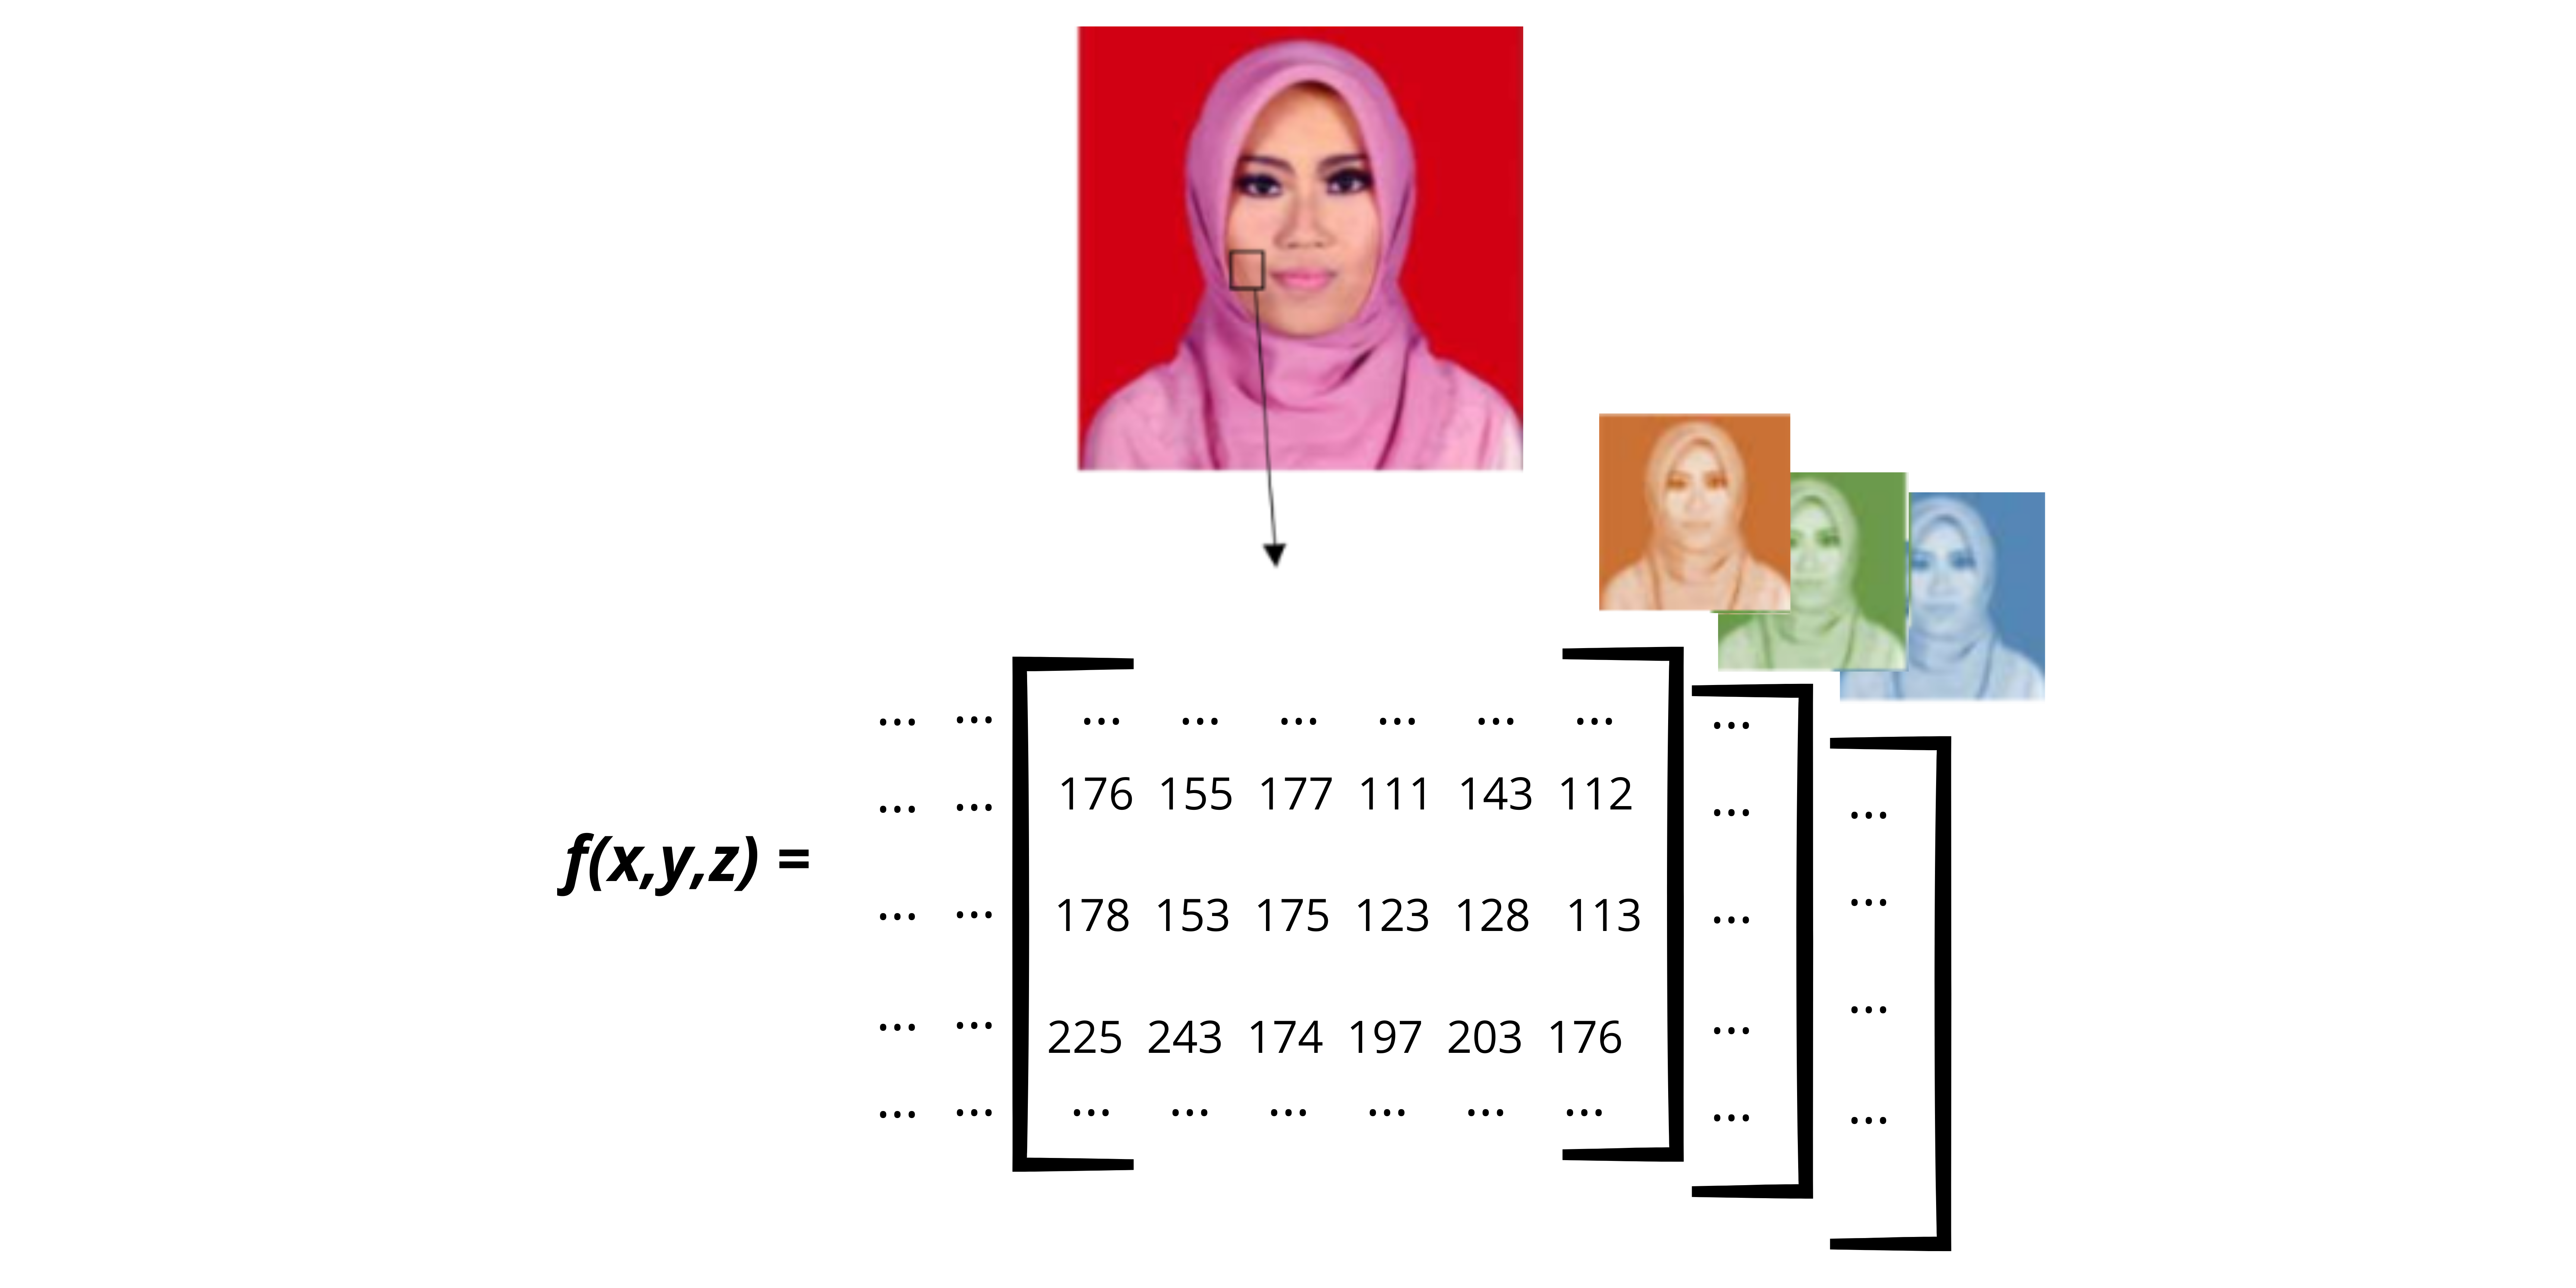
\includegraphics[width=0.85\textwidth]{figures/bab2/citra_digital.png}
      \caption{Sistem Koordinat Matematis Sebuah Citra \cite{Kirana2021}}
      \label{Sistem Koordinat Matematis Sebuah Citra}
    \end{figure}




    
    
    Pada Gambar \ref{Sistem Koordinat Matematis Sebuah Citra} memberikan visualisasi bentuk wajah seorang manusia dengan warna kulit sawo matang dan kerudung pink. Visualisasi wajah manusia tersebut merupakan sebuah kombinasi pixel yang membuat intensitas warna yang di tunjukkan pada fungsi $f(x,y)$. Berdasarkan persamaan tersebut, $f$ diasumsikan sebagai intensitas warna dan $(x,y,z)$ adalah koordinat pada dimensi x dan y pada \textit{layer} z. Sehingga citra sering didefenisikan sebagai sebuah fungsi yang memuat kombinasi intensitas warna dengan koordinat tertentu \cite{Kirana2021}.

\subsection{Akuisisi Citra  Digital}

    Dalam proses pemrosesan gambar digital, persyaratan awal adalah objek gambar digital itu sendiri. Hal ini dicapai melalui langkah akuisisi gambar, di mana gambar digital diperoleh dengan menggunakan alat akuisisi seperti kamera digital, ponsel pintar, mesin pemindai, internet, dll. Alat-alat ini menghasilkan kumpulan data dalam format seperti JPG, PNG, Bitmap, atau yang serupa. Tahap ini juga disebut sebagai tahap pengumpulan dataset \cite{Dewi2018}.
    
    
    Langkah awal lingkungan ditangkap menggunakan sebuah sensor electronik citra yag terbuat dari sensor cahaya CCD \textit{(charge-coupe device}) atau CMOS \textit{(Complementary Metal Oxide Semiconductor)}. Kemudian sensor elektronik mengubah intensitas cahaya dan frekuensi menjadi sebuah gelombang analog. Gelombang analog yang dihasilkan tersebut akan diubah menjadi sinyal digital \cite{putra2010pengolahan}.

\subsection{Augmentasi Citra }

    Augmentasi gambar digital bertujuan untuk memperluas jumlah kumpulan data yang tersedia. Hal ini dilakukan untuk meningkatkan keragaman data tanpa memerlukan proses akuisisi berulang, yang biasanya memakan waktu dan biaya mahal. Salah satu praktik umum dalam proses augmentasi citra digital melibatkan transformasi bentuk data awal yang diperoleh melalui proses akuisisi. Modifikasi yang potensial mencakup memutar gambar digital saat ini pada berbagai sudut, mengubah ruang warna, memperkenalkan \textit{noise}, serta menerjemahkan dan memotong gambar. Tujuannya adalah untuk mencegah \textit{overfitting}, di mana model secara berulang-ulang mengidentifikasi fitur yang sama selama tahap-tahap selanjutnya dari proses pelatihan. Pendekatan ini bertujuan untuk meningkatkan kinerja model ketika ditugaskan untuk mengenali data uji. Ilustrasi augmentasi gambar digital dapat dilihat pada Gambar \ref{Contoh Augmentasi Citra} berikut \cite{Shorten2019, shorten2019survey}.

    
    \begin{figure}[H]
      \centering
      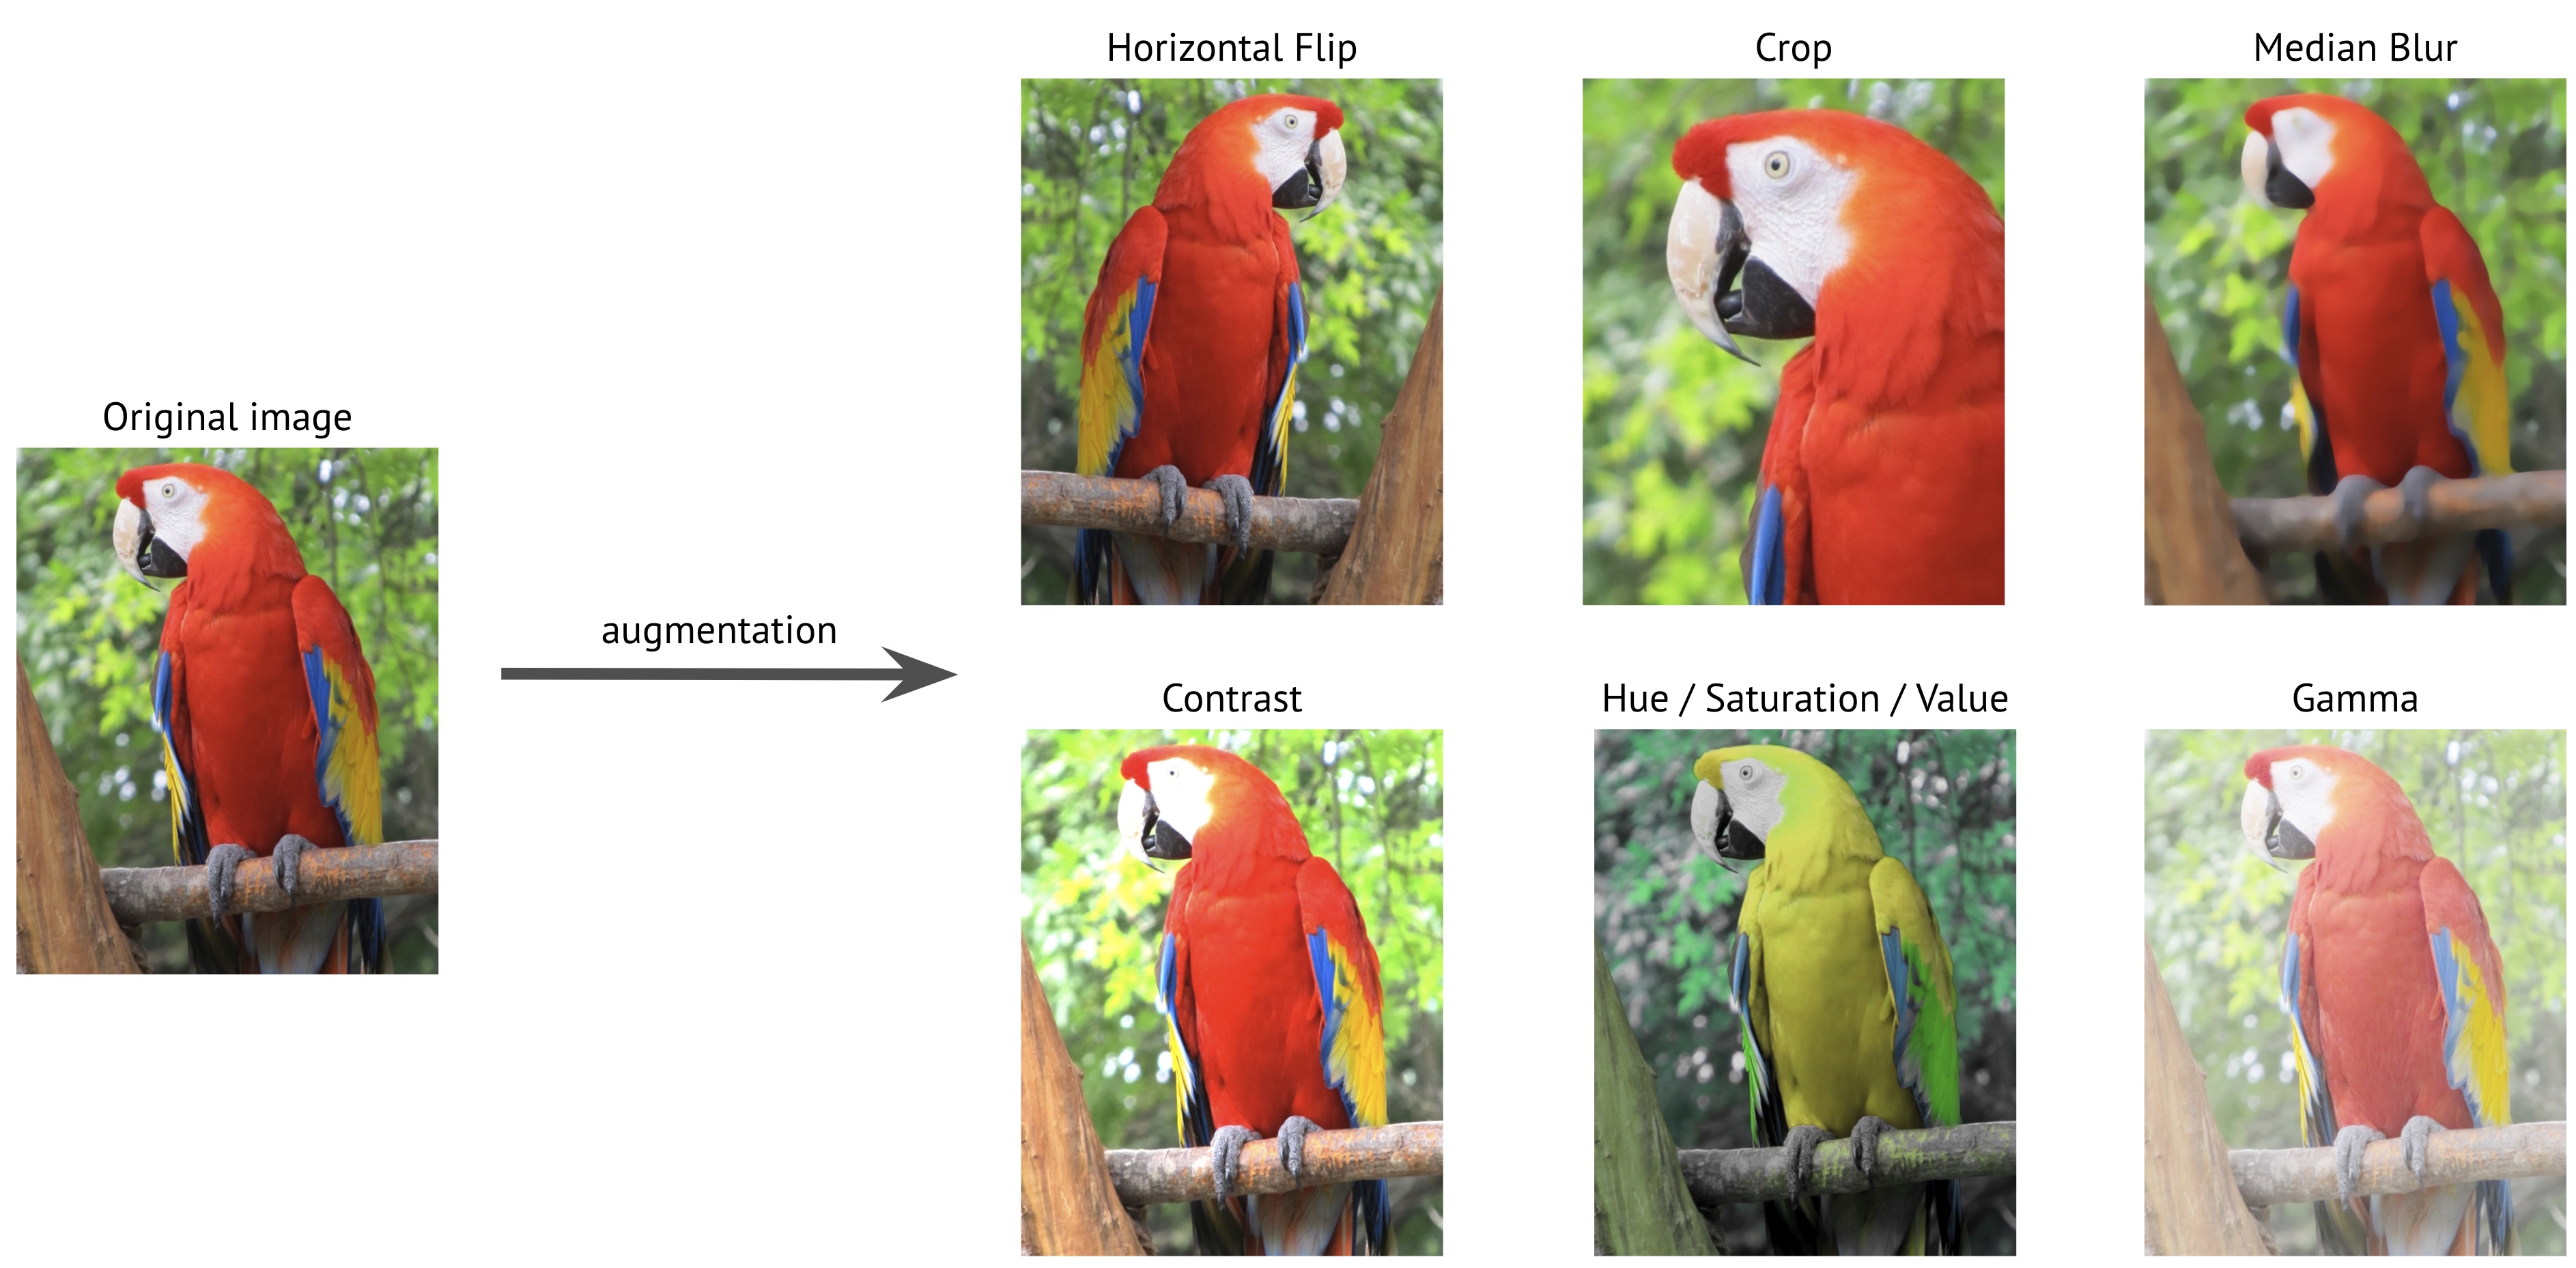
\includegraphics[width=0.85\textwidth]{figures/bab2/augmentation.jpg}
      \caption{Contoh Augmentasi Citra \cite{info11020125}}
      \label{Contoh Augmentasi Citra}
    \end{figure}


    Untuk lebih detail terkait metode-metode augmentasi dijabarkan sebagai berikut

    \subsubsection{\textit{Affine} Transformation}

    
        Dengan menggunakan pendekatan ini, matriks transformasi \textit{affine} dikalikan dengan matriks gambar yang diproses. Transformasi ini menonjol karena kemampuannya untuk mempertahankan bidang, titik, dan garis lurus yang terlihat pada gambar asli. Untuk augmentasi geometris, transformasi \textit{affine} sering digunakan untuk operasi seperti rotasi, translasi, pergeseran, dan penskalaan/pembesaran. Hal ini dimungkinkan karena Persamaan \ref{Affine Transformation} menerapkan gambar yang disediakan \cite{Gonzalez2009}.

   

        \begin{equation}
         \begin{aligned}
            \begin{vmatrix}
                x' \\
                y' \\
                1 \\
            \end{vmatrix} = A \begin{vmatrix}
                x \\
                y \\
                1 \\
            \end{vmatrix} = \begin{vmatrix}
                \alpha_{11} & \alpha_{12} & t_x \\
                \alpha_{21} & \alpha_{22} & t_y \\
                0 & 0 & 1 \\
            \end{vmatrix} \begin{vmatrix}
                x \\
                y \\
                1 \\
            \end{vmatrix}
            \end{aligned} \label{Affine Transformation}
        \end{equation}


        \begin{itemize}
            \item $\alpha_{11}$ dan $\alpha_{22}$ menunjukkan faktor skala untuk sumbu x dan y. Parameter ini mengatur perubahan ukuran objek.

            \item  $\alpha_{21}$ dan $\alpha_{12}$ mewakili rotasi atau \textit{shearing}. Jika  $\alpha_{12} \neq 0$, maka objek akan mengalami rotasi terhadap sumbu x. Sebaliknya, jika $\alpha_{21} \neq 0$, objek akan mengalami rotasi terhadap sumbu y.

            \item $t_x$ dan $t_y$ menunjukkan translasi (geseran) dalam arah x dan y. Parameter ini menentukan seberapa jauh objek digeser dari posisi awalnya.

            \item Baris ketiga $(0,0,1)$ merupakan baris tetap yang memungkinkan representasi vektor homogen (tipe vektor yang dapat mewakili koordinat titik dalam ruang homogen).

            
        \end{itemize}

    
        

        Untuk melakukan augmentasi gambar geometris secara komprehensif, berbagai jenis matriks transformasi \textit{affine} digunakan untuk menyesuaikan augmentasi sesuai dengan persyaratan tertentu. Matriks transformasi \textit{affine} yang sesuai dengan masing-masing teknik, termasuk rotasi, \textit{translation, shearing, zooming} dirinci dalam Tabel  \ref{Matriks Transformasi Afin pada Operasi Lainnya}.
\begin{table}[H]
    \centering
    \caption{Matriks Transformasi \textit{Affine}}
    \label{Matriks Transformasi Afin pada Operasi Lainnya}
    %\scriptsize
    \begin{tabular}{
        >{\raggedright\arraybackslash}m{1.0cm} 
        >{\centering\arraybackslash}m{3.5cm} 
        >{\raggedright\arraybackslash}m{4.5cm}  
        >{\centering\arraybackslash}m{3.0cm}}
        \hline
        \textbf{Teknik} & \textbf{Matriks} & \textbf{Keterangan} & \textbf{Hasil} \\
        \hline \\
        Translasi & 
        \(\begin{bmatrix}
            1 & 0 & 0 \\
            0 & 1 & 0 \\
            t_x & t_y & 1 \\
        \end{bmatrix}\)
        
        & 
        
        Nilai $t_x$ mewakili pergeseran citra sepanjang sumbu $x$, sedangkan nilai $t_y$ mengindikasikan perpindahan citra sepanjang sumbu $y$.
        
        &
        
     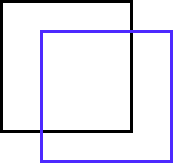
\includegraphics[width=2.0cm, height=2.0cm, keepaspectratio]{figures/bab2/translasi} \\
        
        \textit{Zooming}
        
        & 
        
        \(\begin{bmatrix}
            s_x & 0 & 0 \\
            0 & s_y & 0 \\
            0 & 0 & 1 \\
        \end{bmatrix}\) &
        $s_x$ menunjukkan perubahan skala citra sepanjang sumbu $x$, sementara $s_y$ menggambarkan perubahan skala citra sepanjang sumbu $y$. &
        
\includegraphics[width=2.0cm, height=2.0cm, keepaspectratio]{figures/bab2/zoom.png} \\
        \\
        
        \textit{Shear} & 
        \(\begin{bmatrix}
            1 & sh_y & 0 \\
            sh_x & 1 & 0 \\
            0 & 0 & 1 \\
        \end{bmatrix}\) &
        $sh_x$ adalah nilai skala untuk pergeseran citra sepanjang sumbu $x$, sementara $sh_y$ adalah nilai skala untuk pergeseran citra sepanjang sumbu $y$. &
        
\includegraphics[width=2.0cm, height=2.0cm, keepaspectratio]{figures/bab2/shear.png} \\
        
        \textit{Rotation} & 
        \(\begin{bmatrix}
            \cos \theta & \sin \theta & 0 \\
            -\sin \theta & \cos \theta & 0 \\
            0 & 0 & 1 \\
        \end{bmatrix}\) &
        $\theta$ adalah besar sudut perputaran citra. &
        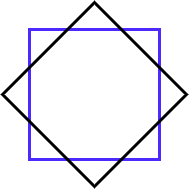
\includegraphics[width=2.0cm, height=2.0cm, keepaspectratio]{figures/bab2/rotasi} \\ 

        \\
        \hline
    \end{tabular}
\end{table}




   

\subsubsection{\textit{Brightness} Dan \textit{Contrast}}

    Praktik membuat gambar dan memodifikasi kecerahan dan kontras untuk setiap gambar baru dikenal sebagai meningkatkan nilai kecerahan dan kontras gambar. Karena dapat meningkatkan performa pengenalan gambar pada model, strategi augmentasi ini sering digunakan dalam penelitian terkait pembelajaran mesin \cite{mikolajczyk2018data}\cite{Yang2022}. Ada beberapa metode untuk menerapkan kedua modifikasi ini. Salah satu metode untuk meningkatkan tingkat kecerahan adalah dengan mengubah gambar RGB menjadi HSV, yang memisahkan tiga saluran warna (h, s, dan v). Saluran \textit{value} (v) nilainya berkisar antara $-50 < v < 50$ yang mengontrol kecerahan gambar, \textit{saturation} (S) mengukur intensitas atau kemurnian warna dan \textit{hue} (h) merepresentasikan jenis warna yang dirasakan manusia, seperti merah, hijau, biru, kuning, dll. Gambar segar dengan kecerahan yang diubah dihasilkan dengan mengubah saluran v yang dimodifikasi kembali menjadi RGB seperti Gambar \ref{Contoh Augmentasi Contrast} \cite{oza2020empirical, Stollnitz1996}.

    \begin{figure}[H]
      \centering
      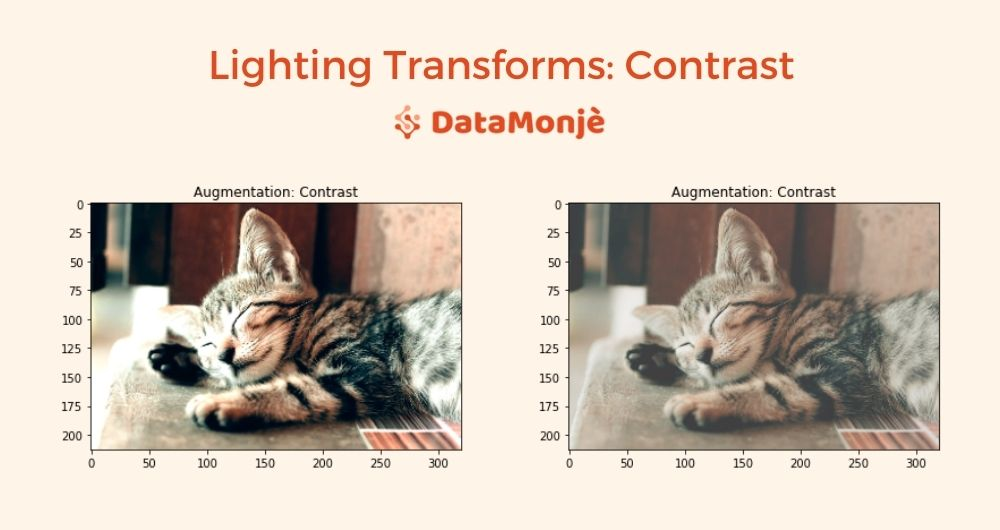
\includegraphics[width=0.75\textwidth]{figures/bab2/Lighting-Transforms-Contrast-augmentation.jpg}
      \caption{Contoh Augmentasi \textit{Brightness} dan\textit{ Contrast} \cite{anand}}
      \label{Contoh Augmentasi Contrast}
     \end{figure} 
    
    Berbagai teknik, termasuk penyesuaian kontras linier, mengubah skala nilai piksel individual, menggunakan metode berbasis histogram, dan teknik berbasis resonansi, dapat digunakan untuk mengubah nilai kontras gambar melalui augmentasi \cite{Bebis2021, Maragatham2015, szeliski2021computer}. Teknik sederhana yang dapat digunakan untuk mengontrol nilai kontras pada suatu gambar dapat dilakukan dengan Persamaan \ref{Augmentasi Nilai Kontras} sebagai berikut.

    
    
    \begin{equation}
      \begin{aligned} 
        g(i, j) = \alpha \cdot f(i, j) + \beta
        \end{aligned}\label{Augmentasi Nilai Kontras}
    \end{equation}


    \textbf{Keterangan:}
      \begin{align*}
        f(x) & : \text{Nilai probabilitas densitas fungsi (PDF) pada titik } x. \\
        g(i, j) & : \text{Nilai piksel pada gambar yang diubah (\textit{output})}. \\
        \alpha & : \text{Faktor kontras}. \\
         f(i, j) & : \text{Nilai piksel pada gambar asli (\textit{input})}.\\
         \beta & : \text{Nilai bias}.\\
    \end{align*}

    Persamaan ini merepresentasikan proses perkalian dan penjumlahan dua buah titik dengan sebuah konstanta. Parameter \textit{gain} dan \textit{bias}, dilambangkan dengan $\alpha$ dan  $\beta$, menentukan nilai kontras dan kecerahan, masing-masing \cite{Szeliski2021}.
    
\subsubsection{\textit{Gaussian Noise}}


     Dengan menggunakan persamaan distribusi normal (juga dikenal sebagai distribusi Gauss dalam Persamaan \ref{Rumus Distribusi Normal (Gaussian)}). Gaussian diterapkan untuk menyempurnakan gambar dengan menambahkan \textit{noise}. Dengan menggunakan metode ini, nilai piksel gambar digital diubah. Dalam kasus tertentu, menambahkan \textit{noise} gaussian ke pengenalan atau klasifikasi gambar memberikan perkiraan model yang mendekati fitur skenario dunia nyata yang sedang dipelajari.
 

    \begin{equation}
        \begin{aligned}
            f(x) = \frac{1}{\sigma \sqrt{2\pi}} \exp\left(-\frac{1}{2} \left(\frac{x - \mu}{\sigma}\right)^2\right)
        \end{aligned}\label{Rumus Distribusi Normal (Gaussian)}
    \end{equation}


    \textbf{Keterangan:}
      \begin{align*}
        f(x) & : \text{Nilai probabilitas densitas fungsi (PDF) pada titik } x \\
        \sigma & : \text{Simpangan baku (standard deviation) distribusi} \\
        \pi & : \text{Konstanta matematika pi dengan nilai } \pi \approx 3.14\\
        \mu & : \text{Rata-rata (mean) distribusi} \\
        \exp & : \text{Fungsi eksponensial} \\
        x & : \text{Nilai variabel acak yang ingin dihitung probabilitasnya} \\
    \end{align*}
    


    
    Variabel x mewakili intensitas nilai yang akan didistribusikan, $\mu$ adalah nilai mean dari distribusi tersebut, dan $\sigma$ adalah standar deviasi dari nilai baru yang dimasukkan ke dalam distribusi citra awal.



\section{\textit{Eye Aspect Ratio} (EAR)}

    Pendeteksian \textit{Eye Aspect Ratio }(EAR) merupakan metode yang digunakan untuk mengukur keterbukaan mata. EAR dihitung dengan menggunakan rasio jarak antara beberapa \textit{landmark} mata \cite{electronics11193183}. Dapat dilihat pada Persamaan \ref{rumus ear} berikut.

    
    \begin{equation}
    \label{rumus ear}
    (\text{EAR}_{\text{left}}, \text{EAR}_{\text{right}}   = \frac{{\| \vec{p}_2 - \vec{p}_6 \| + \| \vec{p}_3 - \vec{p}_5 \|}}{{2 \| \vec{p}_1 - \vec{p}_4 \|}})
    \end{equation}

    \begin{equation}
    \text{EAR} = \frac{1}{2}(\text{EAR}_{\text{left}} + \text{EAR}_{\text{right}})
    \end{equation}


    \textbf{Keterangan:}
    \begin{align*}
        \vec{p}_i & : \text{Vektor posisi dari titik ke-i} \\
        \|\vec{p}_2 - \vec{p}_6\| & : \text{Jarak antara titik } \vec{p}_2 \text{ dan } \vec{p}_6 \\
        \|\vec{p}_3 - \vec{p}_5\| & : \text{Jarak antara titik } \vec{p}_3 \text{ dan } \vec{p}_5 \\
        \|\vec{p}_1 - \vec{p}_4\| & : \text{Jarak antara titik } \vec{p}_1 \text{ dan } \vec{p}_4 \\
    \end{align*}
    

    Pada persamaan EAR dijelaskan diatas, di mana $\vec{p}_1$ hingga $\vec{p}_6$ mewakili lokasi
     \textit{landmark 2D} pada retina. $\vec{p}_2, \vec{p}_3, \vec{p}_5,$ dan $\vec{p}_6$ digunakan 
     untuk mengukur tinggi mata, sedangkan $\vec{p}_1$ dan $\vec{p}_4$ digunakan untuk mengukur lebar mata. 
     Saat mata tertutup, nilai EAR dengan cepat turun hingga hampir nol, berbeda dengan saat mata terbuka, 
     yang nilai EARnya tetap konstan. Hal ini digambarkan pada Gambar \ref{Ilustrasi Perhitungan Nilai EAR} berikut.

    \begin{figure}[H]
      \centering
      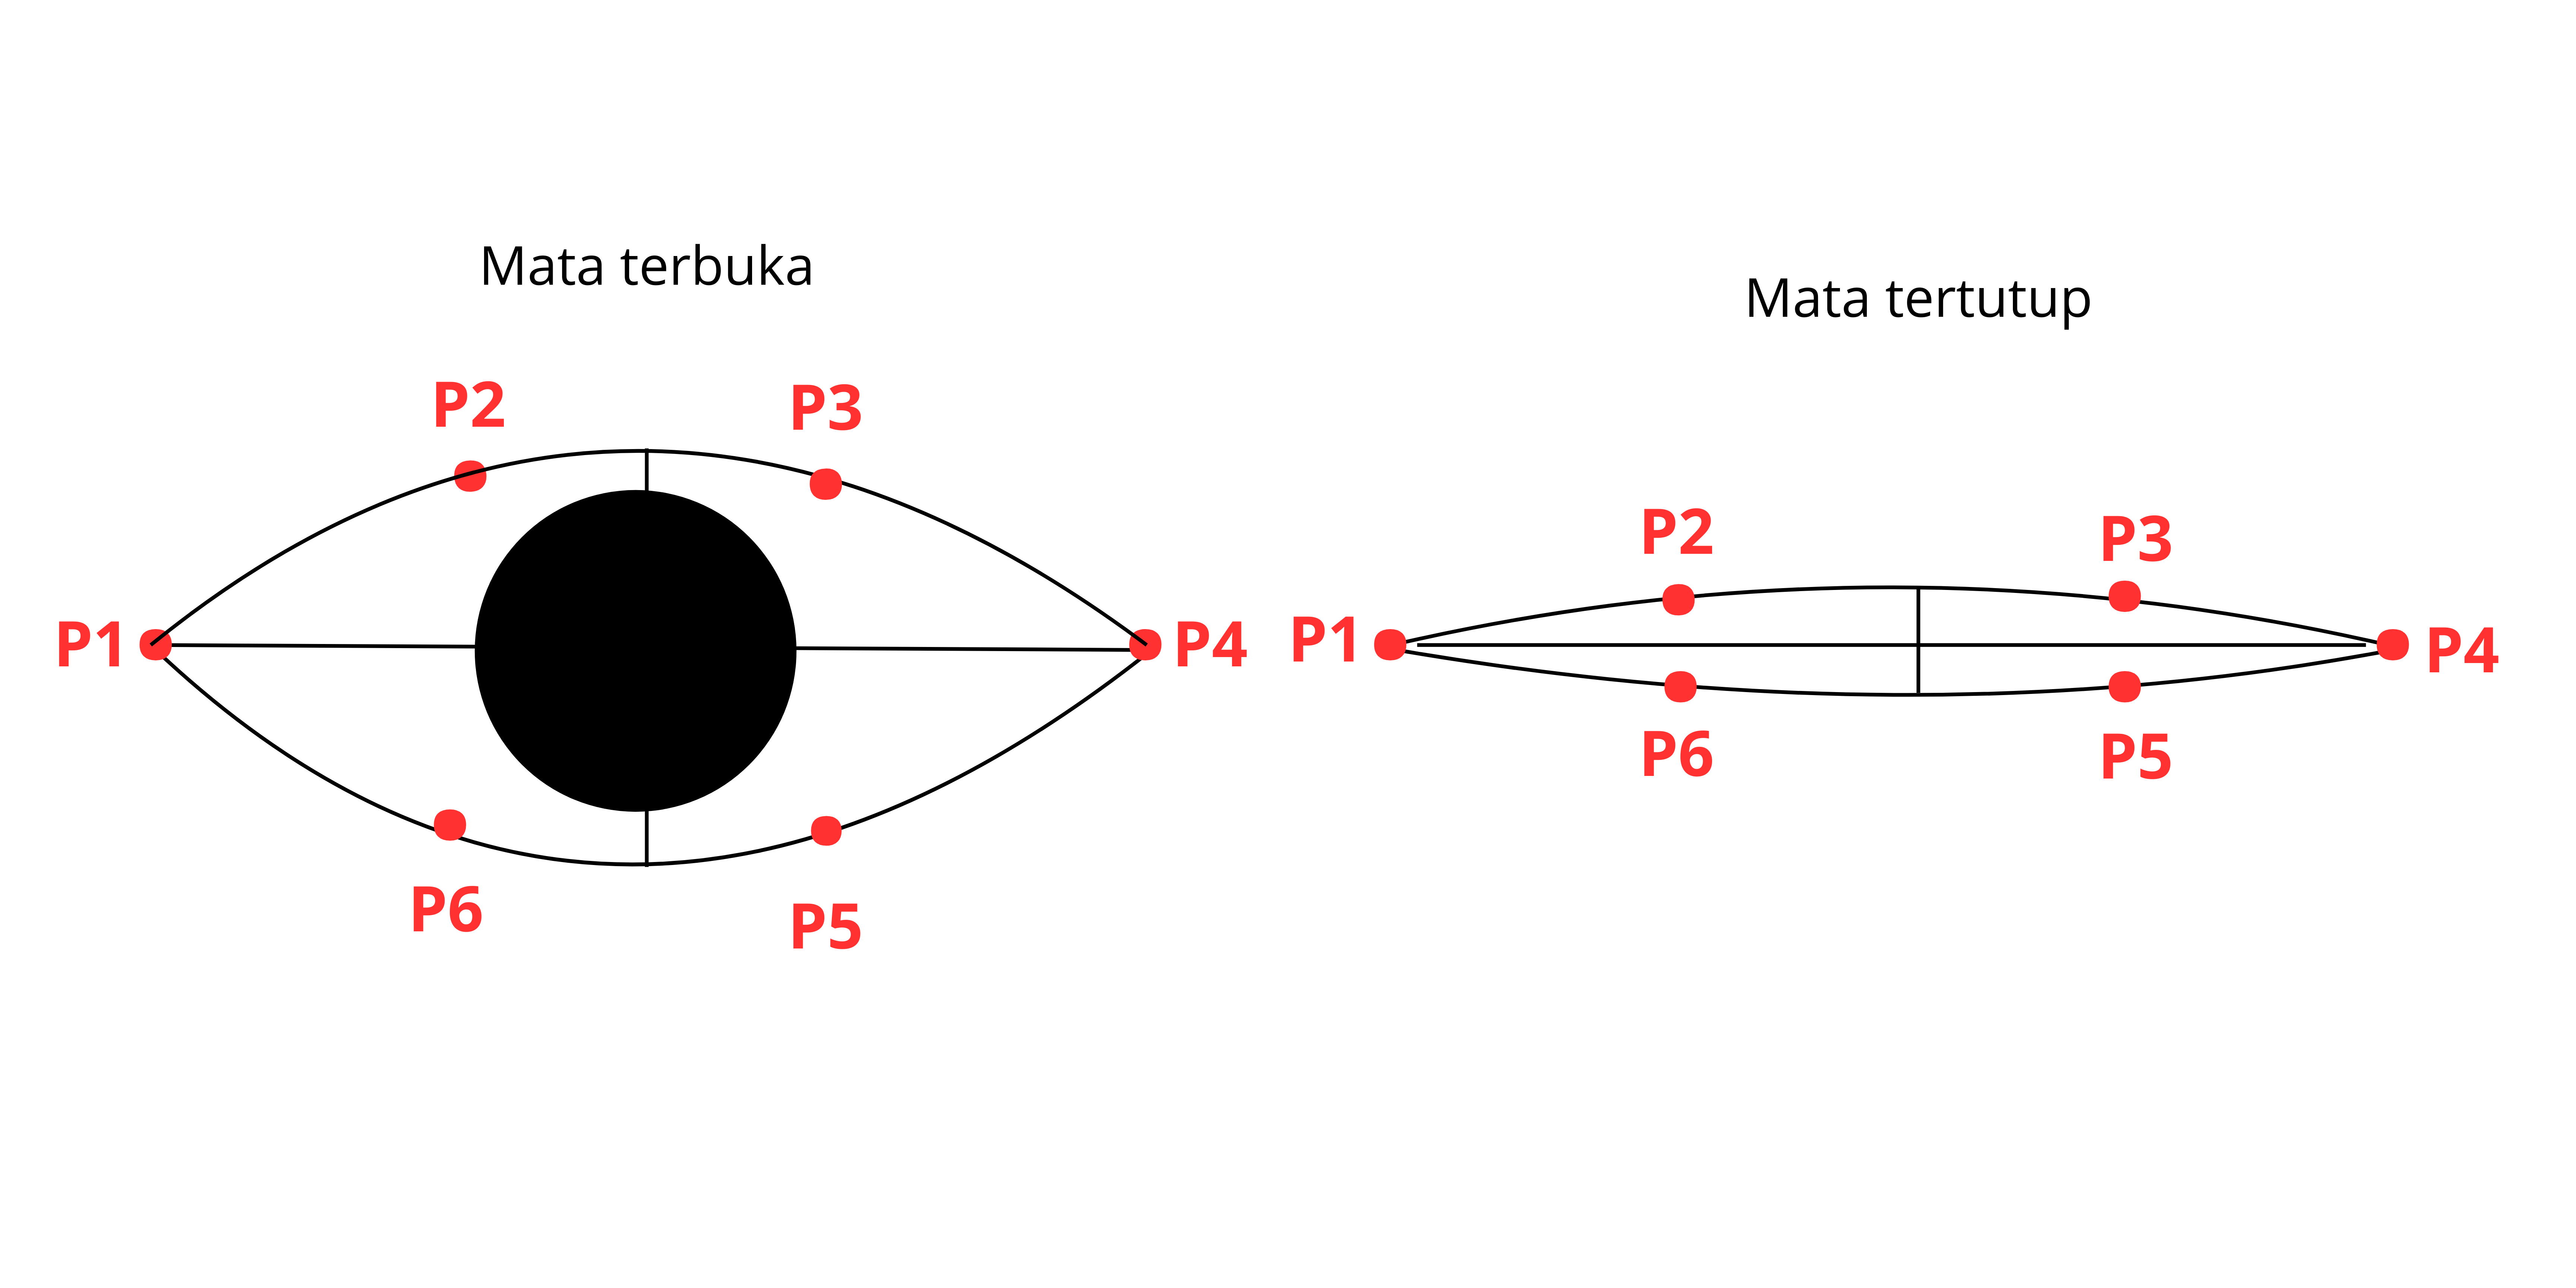
\includegraphics[width=0.8\textwidth]{figures/bab2/EAR.png}
      \caption{Ilustrasi Perhitungan Nilai EAR}
      \label{Ilustrasi Perhitungan Nilai EAR}
    \end{figure}
    
     untuk mengukur tingkat kesalahan deteksi yang terjadi. Tingkat kesalahan deteksi dapat memberikan informasi berharga mengenai akurasi dalam mengidentifikasi kondisi yang benar. Kesalahan deteksi dapat dihitung menggunakan Persamaan \ref{rumus error} berikut.


    \begin{equation}
        \label{rumus error}
        \begin{aligned}
        \text{\textit{error}} = \left(\frac{\text{FP}}{\text{TP + FP}}\right) \times 100\%
        \end{aligned}
    \end{equation}

       \textbf{Keterangan:}
      \begin{align*}
        TN & : \text{Benar melakukan prediksi} \\
        FN & : \text{Salah melakukan prediksi} \\
    \end{align*}

   

\section{\textit{Mouth Aspect Ratio} (MAR)}

Pendeteksian \textit{Mouth Aspect Ratio} (MAR) merupakan metode yang digunakan untuk mengukur lebar terbuka mulut. MAR dihitung dengan menggunakan rasio jarak antara beberapa \textit{landmark} mulut. Koordinat digunakan untuk mewakili mulut. Dimulai dari
sudut kiri mulut, yang tengara ditandai dalam searah jarum jam di sekitar sisanya
wilayah tersebut. MAR diukur dengan membagi vertikal jarak antara bibir atas dan bibir bawah dengan horizontal jarak antara kedua bibir \cite{inproceedings, jimaging9050091}. Dapat dilihat pada Persamaan \ref{rumus mar} berikut.


    \begin{figure}[H]
      \centering
      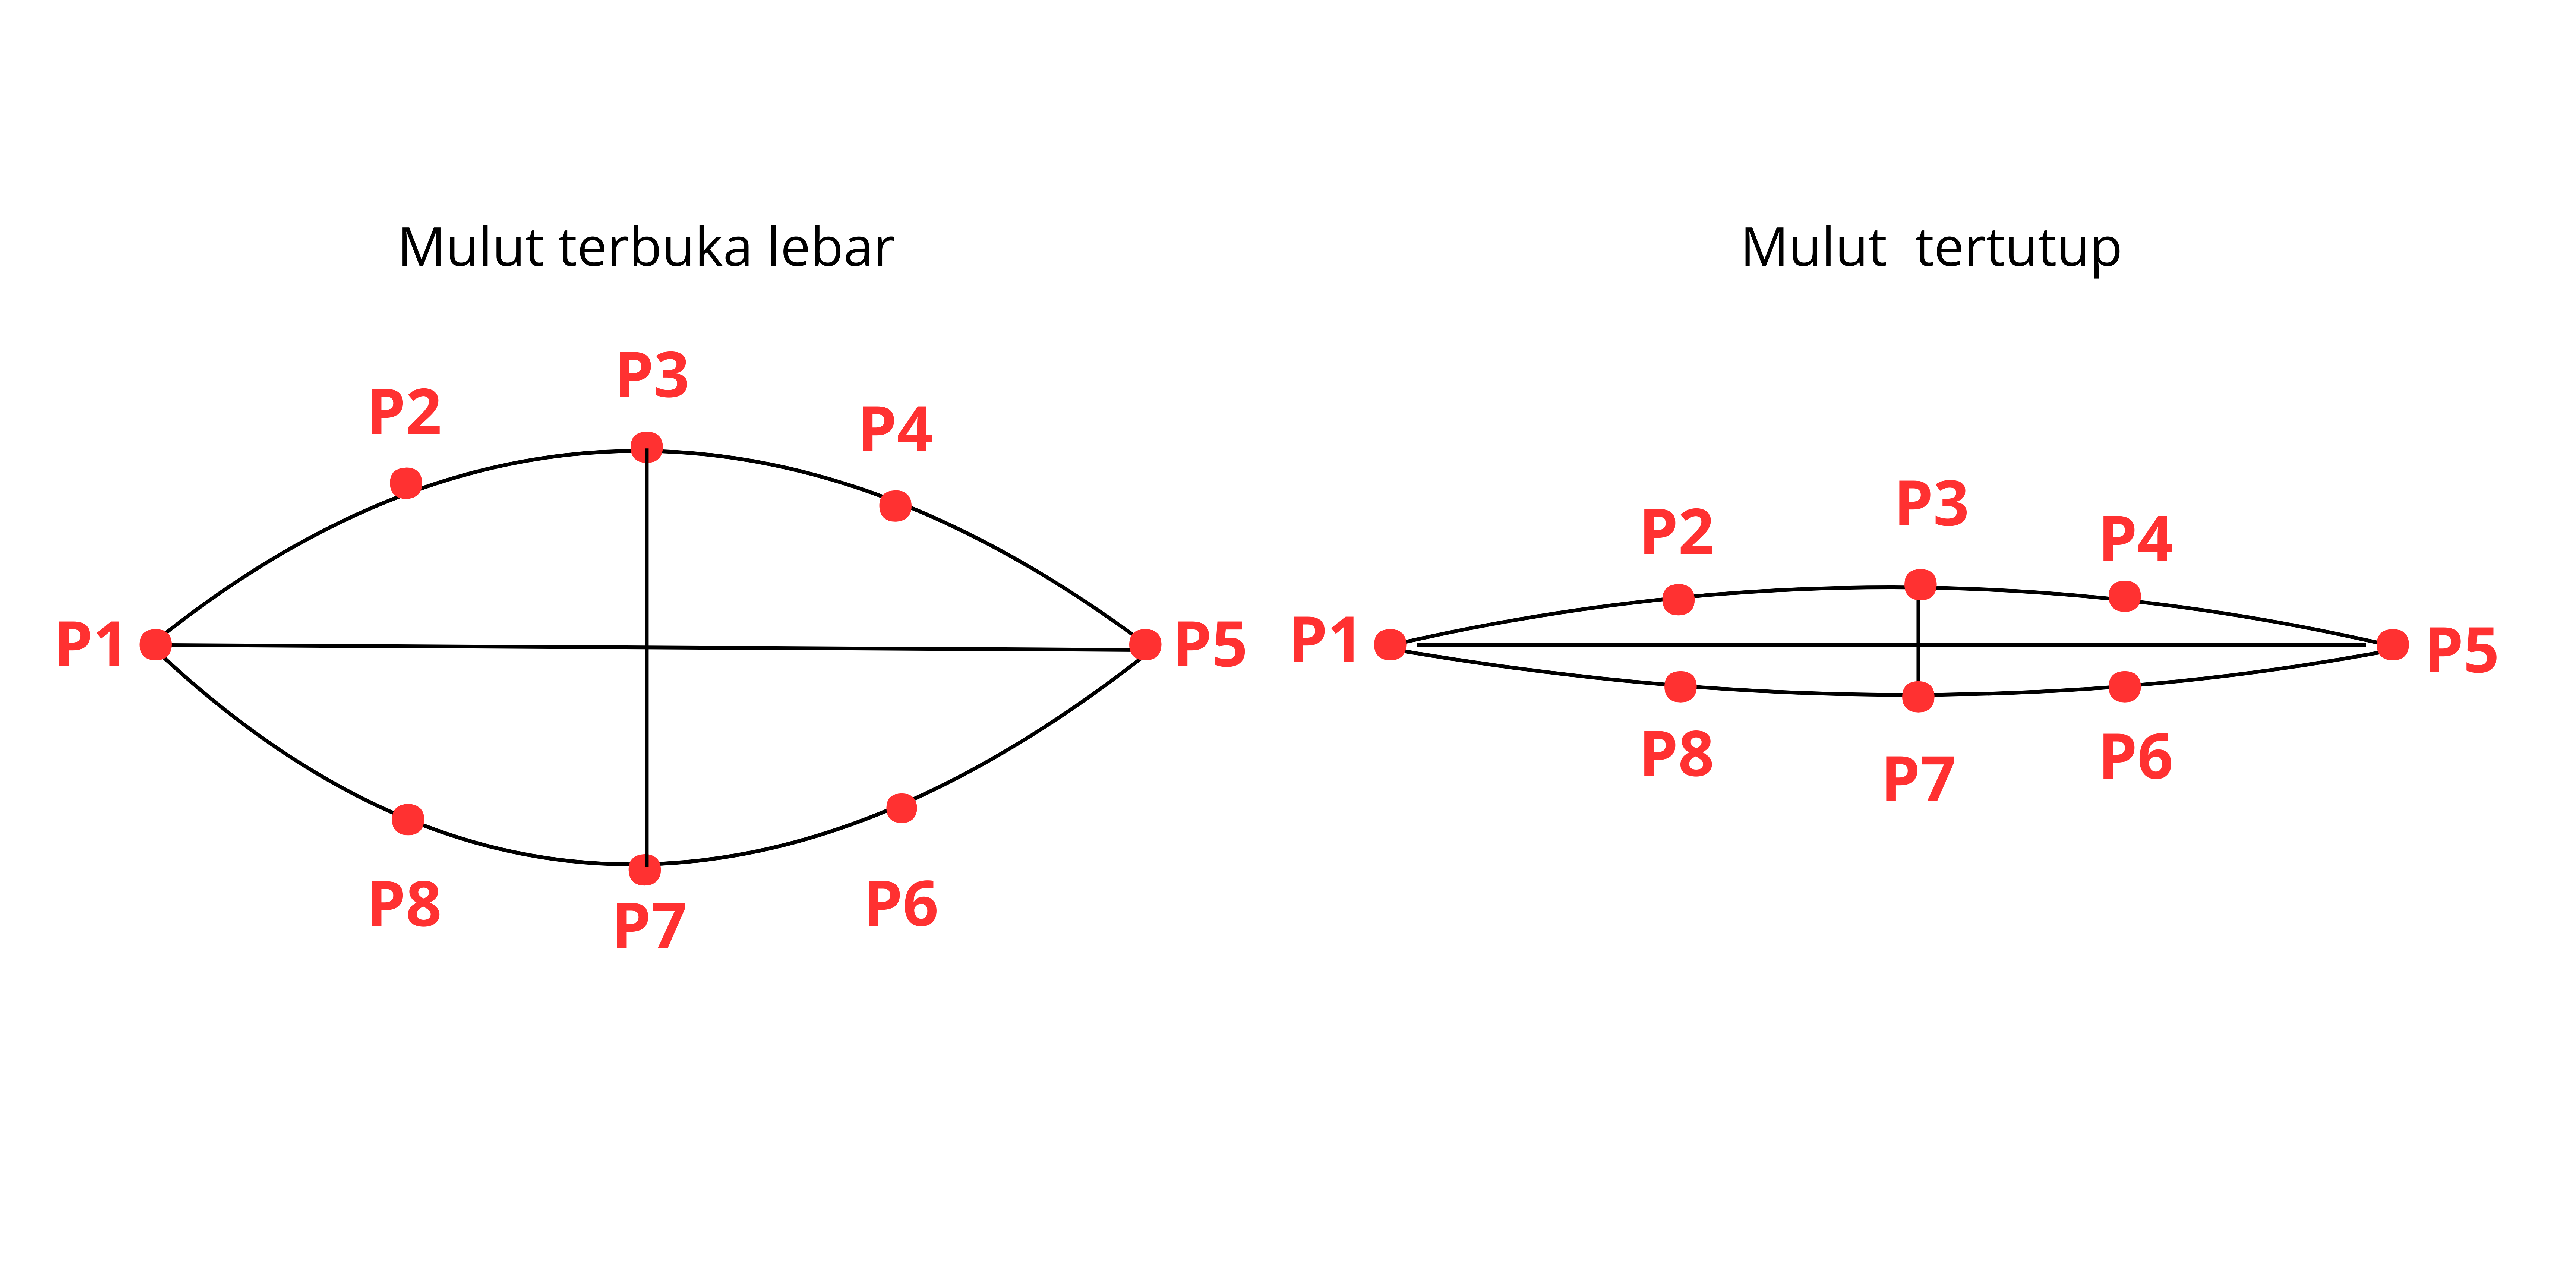
\includegraphics[width=0.8\textwidth]{figures/bab2/mar.png}
      \caption{Ilustrasi Perhitungan Nilai MAR}
      \label{Ilustrasi Perhitungan Nilai MAR}
    \end{figure}

     \begin{equation}
    \label{rumus mar}
    \text{MAR} = \frac{\| \vec{p}_2 - \vec{p}_8 \| + \| \vec{p}_3 - \vec{p}_7 \| + \| \vec{p}_4 - \vec{p}_6 \| }{3 \| \vec{p}_5 - \vec{p}_1 \|}
\end{equation}


      \textbf{Keterangan:}
      
    \begin{align*}
        \vec{p}_i & : \text{Vektor posisi dari titik ke-i} \\
        \|\vec{p}_2 - \vec{p}_8\| & : \text{Jarak antara titik } \vec{p}_2 \text{ dan } \vec{p}_8 \\
        \|\vec{p}_3 - \vec{p}_7\| & : \text{Jarak antara titik } \vec{p}_3 \text{ dan } \vec{p}_7 \\
        \|\vec{p}_4 - \vec{p}_6\| & : \text{Jarak antara titik } \vec{p}_4 \text{ dan } \vec{p}_6 \\
        \|\vec{p}_5 - \vec{p}_1\| & : \text{Jarak antara titik } \vec{p}_5 \text{ dan } \vec{p}_1 \\
    \end{align*}



    

\section{\textit{Convolutional Neural Network} (CNN)}

    \textit{Convolutional Neural Network} (CNN) adalah sub tipe \textit{Artificial Neural Network} (ANN) yang dibuat khusus untuk mengatasi tantangan terkait data dua dimensi (2D). \textit{Convolutional Neural Network} (CNN) menjalani proses pembelajaran berdasarkan data pelatihan yang diberikan. Mirip dengan jaringan saraf manusia ketika mencoba untuk memahami atau mengenali sesuatu, proses pembelajaran ini menghasilkan pola yang sesuai. Selanjutnya, setelah mengekstraksi data fitur dari kumpulan data pelatihan, data tersebut dapat diterapkan untuk mengatasi masalah klasifikasi. Istilah pada CNN dibahas pada  berikut  \cite{Alzubaidi2021}. 
    
  \begin{figure}[H]
      \centering
      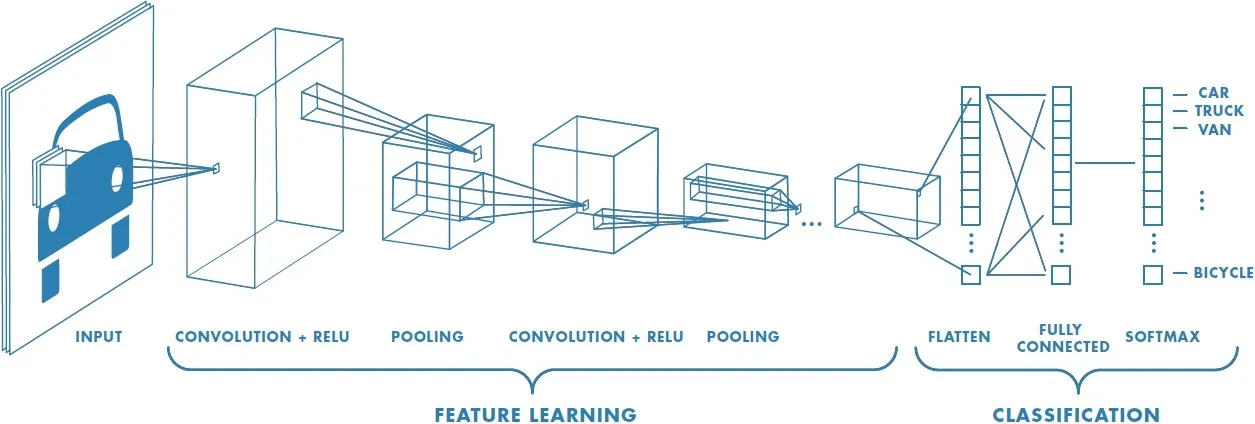
\includegraphics[width=1\textwidth]{figures/bab2/arsitektur cnn.jpg}
      \caption{Arsitektur \textit{Convolutional Neural Network} (CNN) \cite{Prabhu}}
      \label{Arsitektur CNN}
    
    \end{figure}

    Secara garis besar proses pada \textit{Convolutional Neural Network} (CNN) terbagi menjadi dua garis besar yaitu \textit{feature learning} dan \textit{classification}. Pada \textit{input layer} terdapat nilai piksel dan jumlah chanel dari gambar yang dimasukkan, Proses \textit{convolution} menghasilkan \textit{feature map} 
    yang diperoleh dengan menerapkan \textit{filter} berupa matriks.  Di sini, Nilai \textit{feature map} diubah berdasarkan \textit{activation function} yang digunakan seperti ReLU, softmax dan lain-lain. Setelah melewati berbagai proses selanjutkan digunakan \textit{pooling layer} yang bertujuan untuk mengurangi resolusi gambar, namun tidak menghilangkan informasi penting yang dimiliki. Sehingga hal ini dapat mengurangi jumlah parameter dan mempercepat proses klasifikasi. 

    Pada lapisan terakhir terdapat \textit{fully connected layer} dimana semua neuron dari lapisan sebelumnya terhubung pada neuron lapisan berikutnya. Lapisan yang terhubung pada \textit{fully connected layer} sebelumnya telah berubah berubah mejadi data satu dimensi yang disebut dengan \textit{flatten}. \textit{Layer}
    menggunakan semua nilai dan fitur yang telah dipelajari untuk membuat sebuah keputusan sesuai dengan kelas yang telah kita defenisikan sebelumnya.


\section{\textit{Layer}}

Pada \textit{Convolutional Neural Network} (CNN) terdapat beberapa \textit{layer} atau lapisan yang disusun menjadi beberapa blok. \textit{Layer} pada setiap blok ini berfungsi untuk melakukan proses pengolahan data, untuk lebih detailnya dijelaskan pada subbab selanjutnya.


\subsection{\textit{Convolution}}

    Dalam jaringan CNN, lapisan \textit{input} berfungsi sebagai tahap awal yang menerima gambar, sementara lapisan \textit{output} menghasilkan label hasil prediksi. Salah satu tahap penting dalam ekstraksi fitur adalah penggunaan \textit{convolution layer}, yang diposisikan di awal untuk menerima \textit{input} dalam bentuk gambar. \textit{Convolution} merupakan jenis operasi linear khusus dan biasanya menjadi lapisan
    pertama pada model CNN yang disebut sebagai \textit{convolution layer}. Operasi pada
    \textit{convolution} berguna untuk mengubah suatu fungsi menjadi fungsi yang lain. Proses \textit{convolution} akan melakukan konversi
    beberapa data yang telah diinisialisasikan melalui \textit{kernel} kemudian ditangkap
    menjadi ukuran \textit{stride} yang telah ditetapkan.
    Operasi yang dilakukan pada lapisan ini mirip dengan operasi konvolusi, yang melibatkan penggabungan berbagai nilai piksel lokal melalui \textit{filter linier}. \textit{Filter} ini berfungsi sebagai reseptor atau penerima neuron. Lapisan yang mendasari arsitektur CNN dirancang untuk mengekstrak fitur atau informasi dari gambar yang diberikan. Berikut ilustrasi proses pergeseran pada \textit{convolution layer} yang di tujukan pada Gambar \ref{Ilustrasi Proses Pergeseran Filter Pada Convolutional Layer} berikut \cite{Dewi2018}.

  \begin{figure}[H]
      \centering
      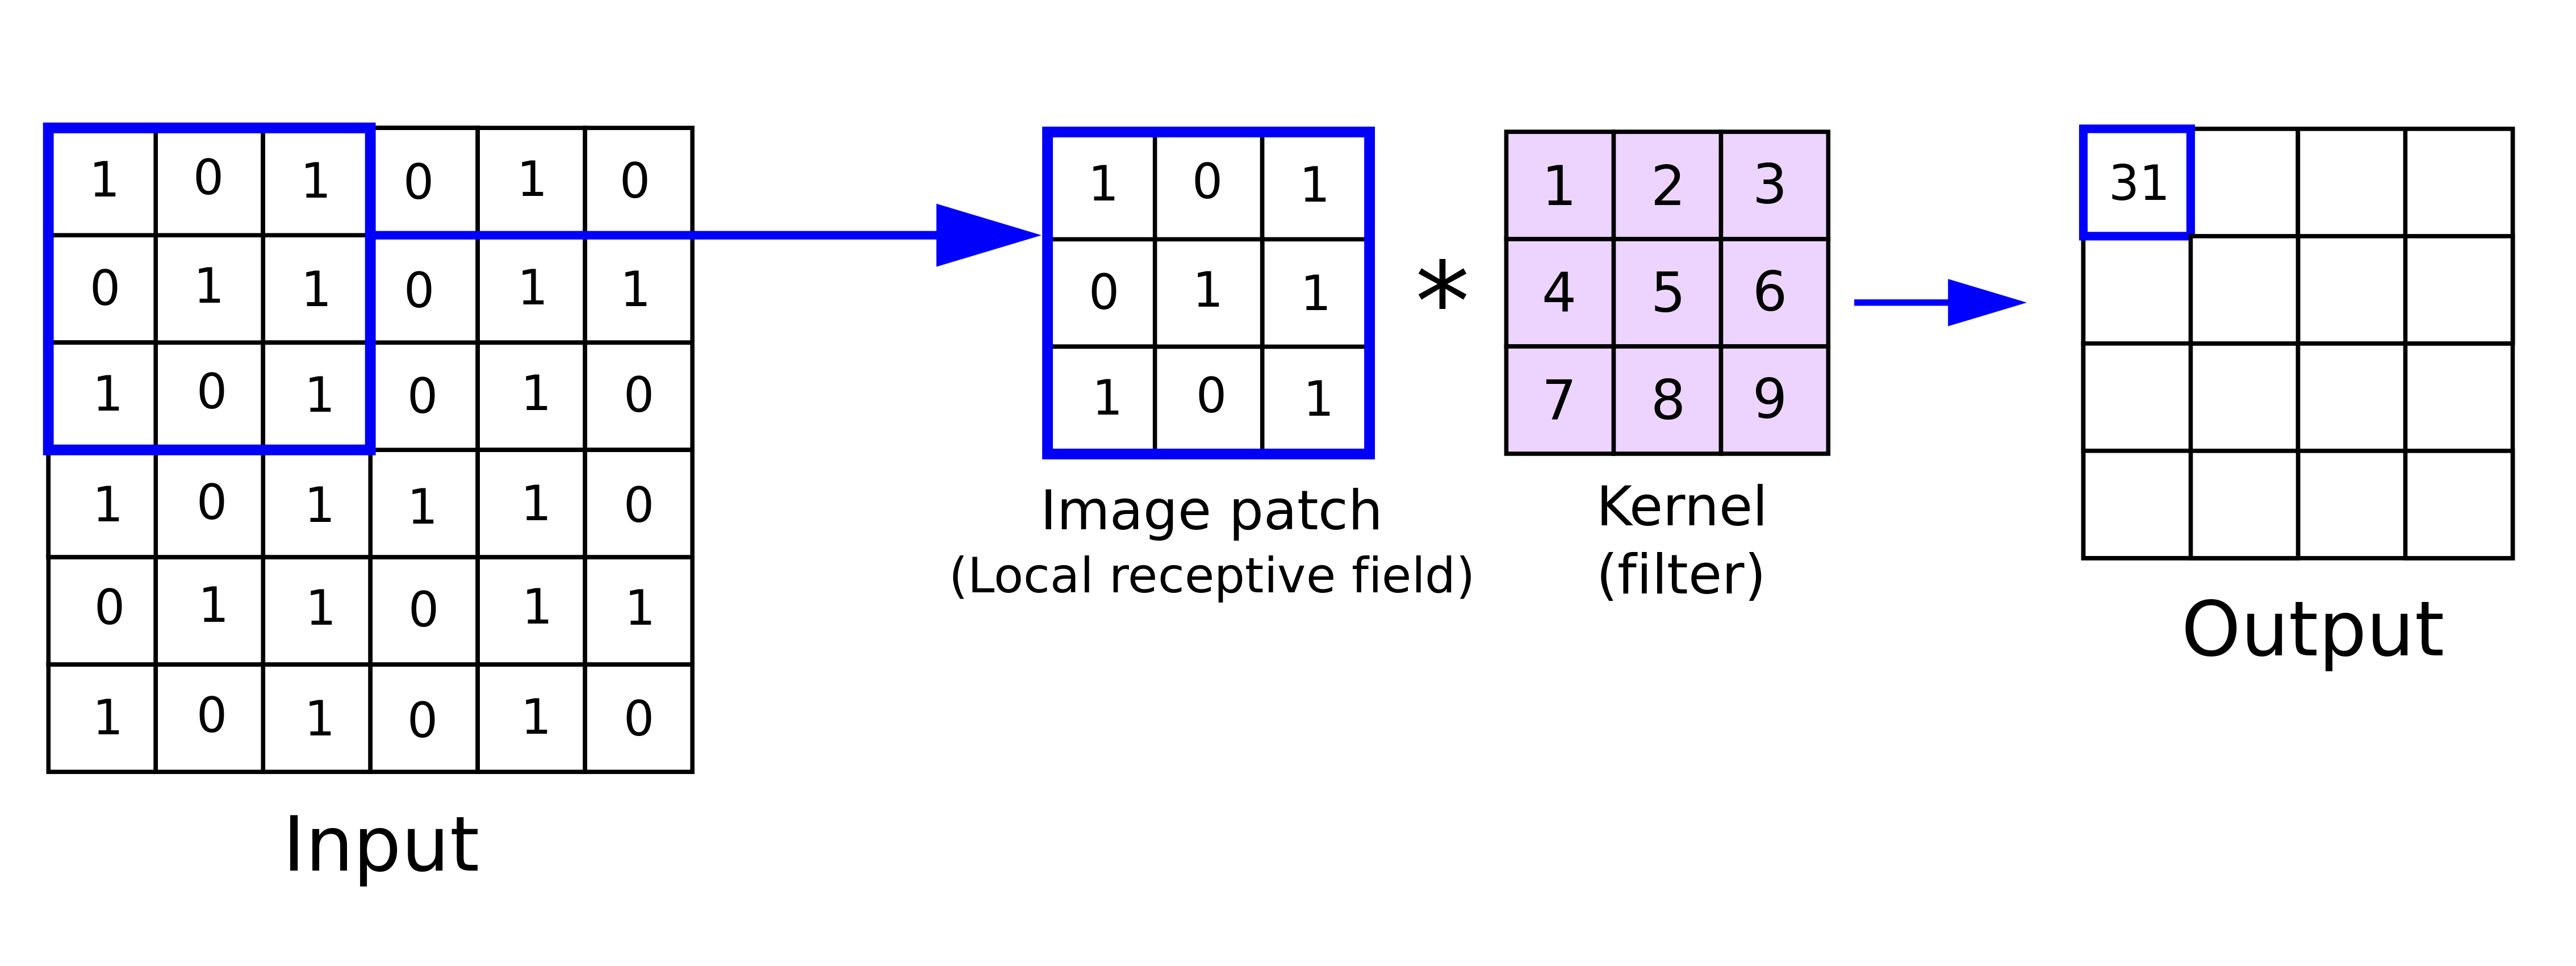
\includegraphics[width=0.8\textwidth]{figures/bab2/cnn.png}
      \caption{Ilustrasi Proses Pergeseran \textit{Filter} \cite{Reynolds}}
      \label{Ilustrasi Proses Pergeseran Filter Pada Convolutional Layer}
    
 \end{figure}


\subsection{\textit{Maxpooling}}

    Lapisan \textit{max pooling} bertanggung jawab untuk menangani matriks \textit{output} dari lapisan sebelumnya, mengurangi ukuran gambar sambil mempertahankan nilai fitur yang penting. Hal ini dilakukan dengan memilih nilai maksimum dari \textit{output} yang dihasilkan oleh lapisan sebelumnya. Pendekatan ini memungkinkan model untuk melakukan proses generalisasi dengan cepat \cite{Gholamalinezhad2020, Nagi2011MaxpoolingCN}. Ilustrasi dari proses \textit{max pooling} ditampilkan pada Gambar \ref{Proses Pada Max Pooling Layer} berikut.


    \begin{figure}[H]
      \centering
      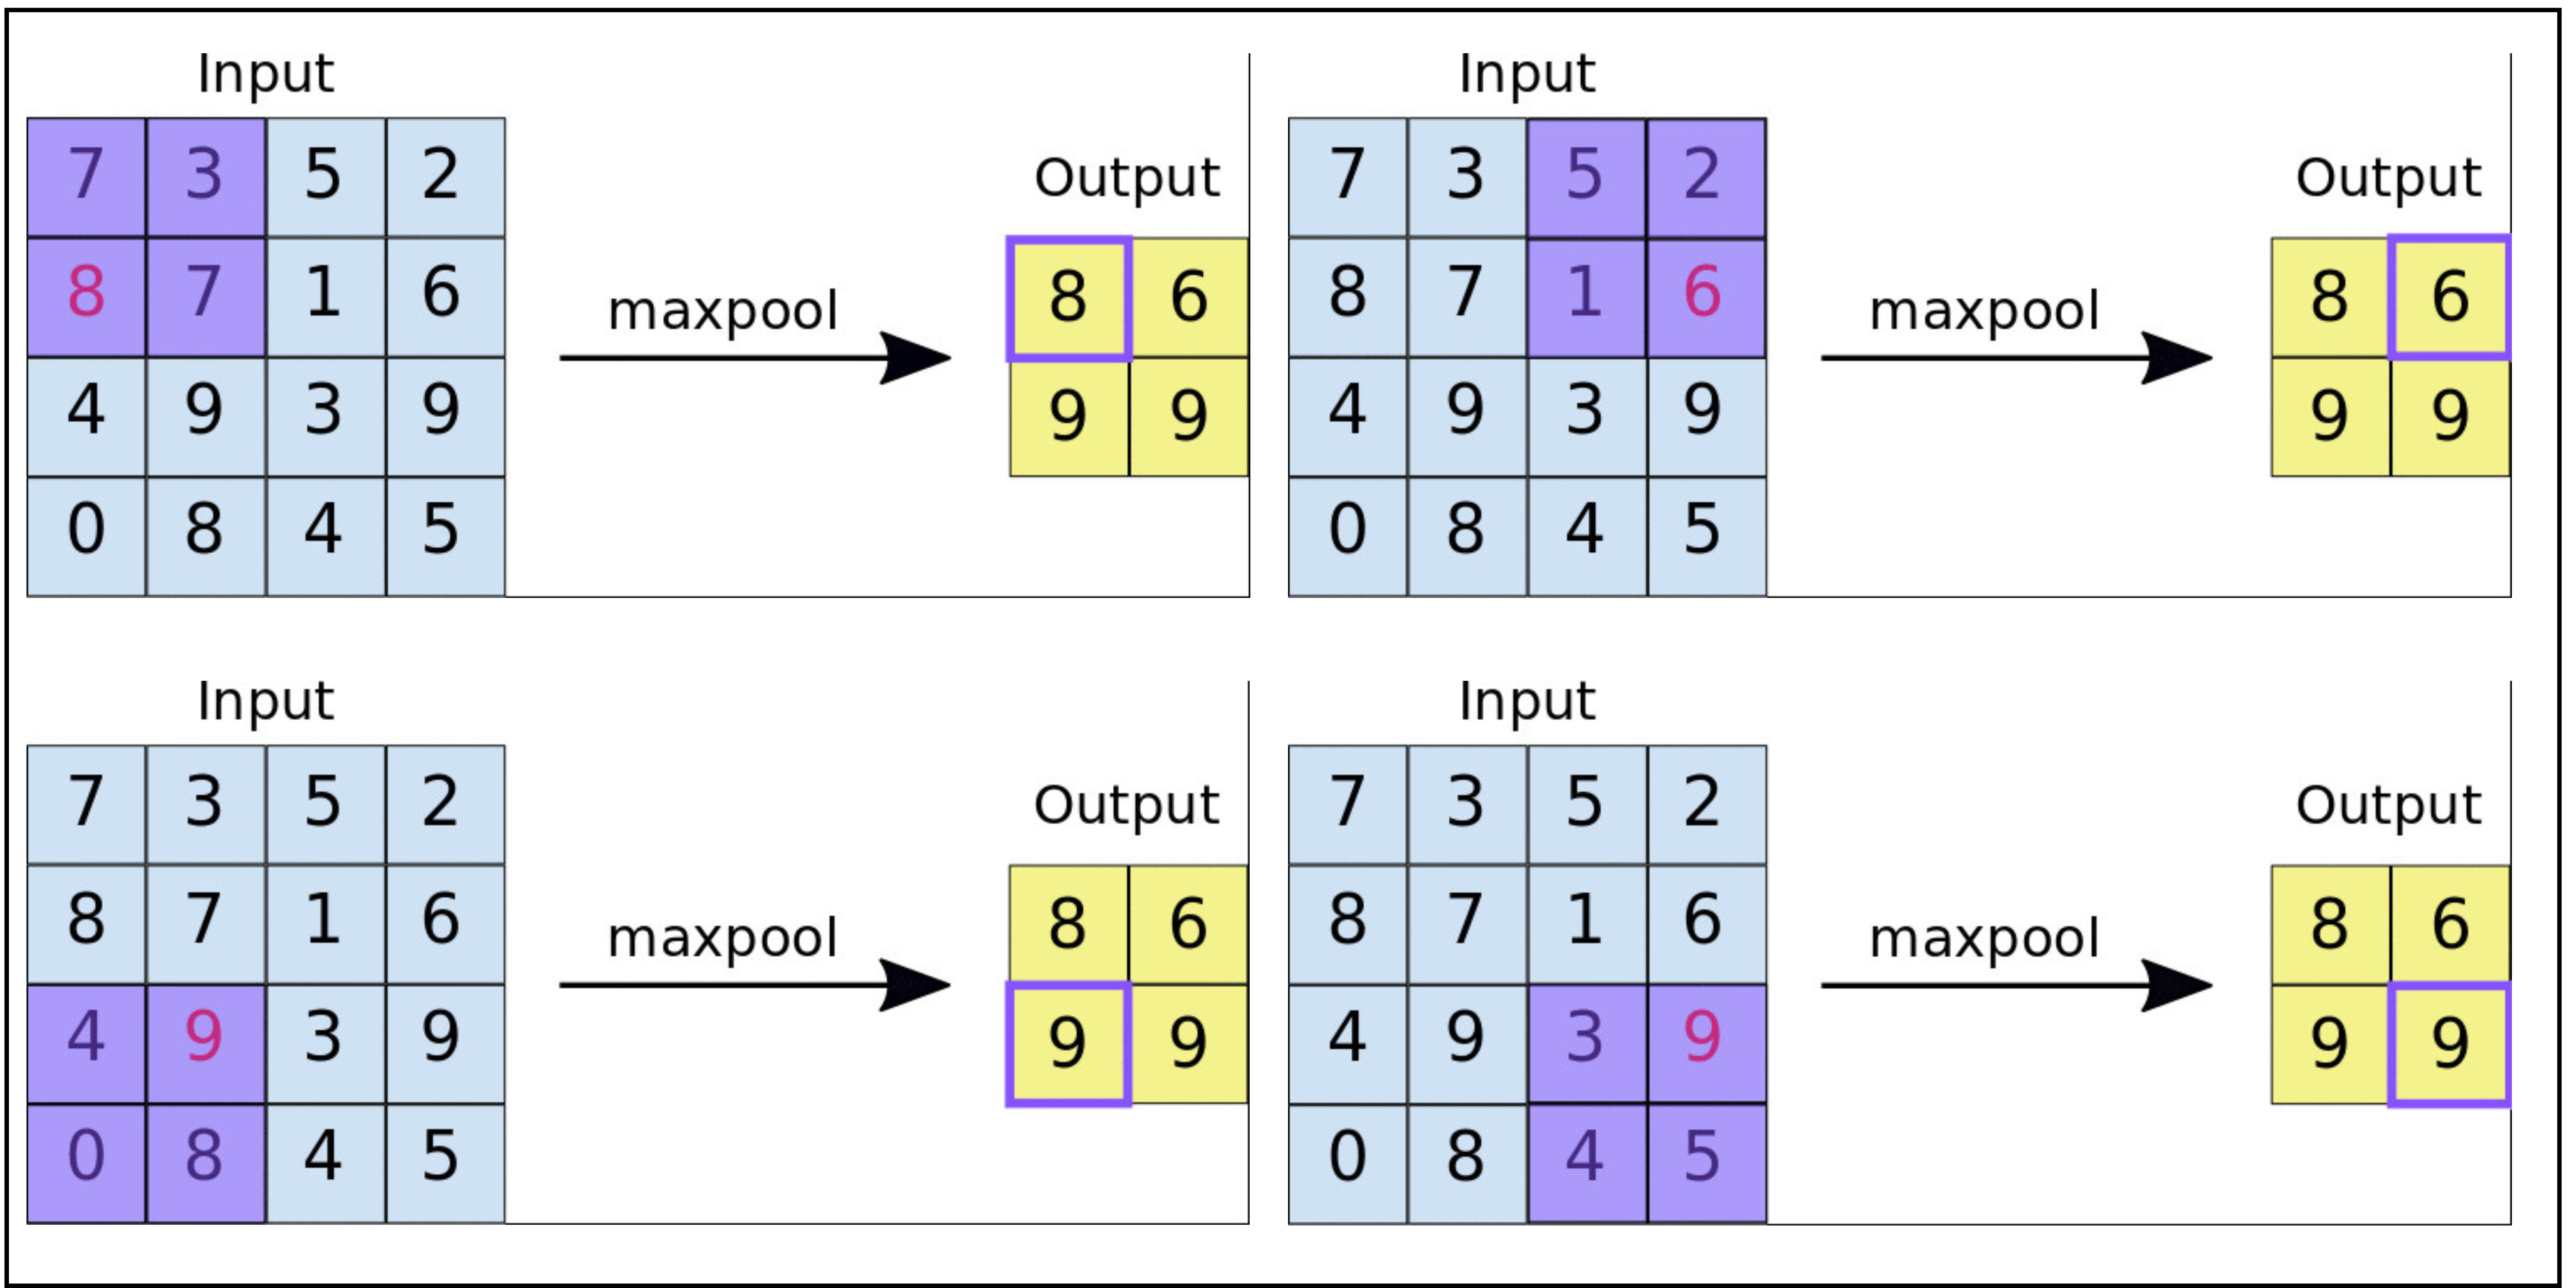
\includegraphics[width=0.75\textwidth]{figures/bab2/pool.png}
      \caption{Proses Pada \textit{Max Pooling Layer} \cite{fiki}}
      \label{Proses Pada Max Pooling Layer}
    \end{figure}

\subsection{\textit{Dropout}}

    Banyak lapisan tersembunyi yang biasanya disertakan dalam model \textit{deep learning}, yang membuatnya lebih mudah untuk memahami interaksi yang kompleks antara \textit{input} dan \textit{output}. \textit{Overfitting} adalah masalah yang umum terjadi meskipun ada manfaatnya, terutama pada dataset yang kecil \cite{Srivastava2014}. Untuk mengatasi hal ini, banyak strategi yang telah dikembangkan salah satunya adalah \textit{dropout}. Selain mencegah \textit{overfitting}, lapisan \textit{dropout} secara efektif menggabungkan beberapa jaringan saraf yang terhubung. Hal ini dilakukan dengan menggabungkan lapisan tersembunyi dengan lapisan lain sambil menghapusnya secara bebas dan sesaat \cite{Srivastava2014}. Pada Gambar \ref{Proses Pada Dropout Layer} berikut menunjukkan proses \textit{dropout layer}.

    \begin{figure}[H]
      \centering
      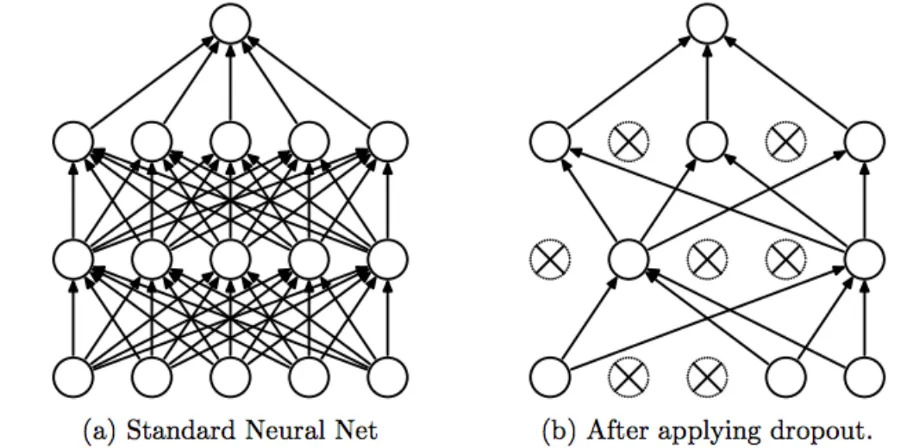
\includegraphics[width=0.70\textwidth]{figures/bab2/drop out.jpg}
      \caption{Proses Pada \textit{Dropout Layer} \cite{ida}}
      \label{Proses Pada Dropout Layer}
    
    \end{figure} 

    
\subsection{\textit{Fully Conected}}

    Lapisan yang terhubung sepenuhnya, juga dikenal sebagai \textit{Multi-Layer Perceptron} (MLP), membangun koneksi antara semua neuron aktivasi di lapisan sebelumnya dan lapisan berikutnya. Lapisan ini mengubah peta fitur yang disajikan sebagai \textit{array} multidimensi menjadi vektor melalui proses perataan, memastikan bahwa setiap aktivasi dari lapisan sebelumnya terhubung secara efektif ke lapisan berikutnya. Umumnya digunakan dalam MLP untuk klasifikasi data, lapisan terhubung sepenuhnya berbeda dari lapisan \textit{convolutional} karena neuron-nya terhubung ke seluruh masukan, menyerupai struktur jaringan saraf manusia yang saling berhubungan. Terlepas dari perbedaan ini, kedua lapisan menjalankan operasi perkalian matriks titik dalam prosesnya \cite{Dewi2018}.

    





\section{\textit{Hyperparameter}}

    \textit{Hyperparameter} dalam CNN merupakan parameter yang tidak secara langsung dipelajari oleh model selama proses \textit{training}. Parameter-parameter ini perlu ditentukan sebelum proses \textit{training} dan memiliki pengaruh signifikan terhadap performa akhir model. Pemilihan nilai \textit{hyperparameter} yang tepat merupakan langkah krusial dalam mengoptimalkan performa CNN.

 \subsection{\textit{Padding}}


    Salah satu parameter dalam CNN adalah \textit{padding}, juga dikenal sebagai \textit{zero padding}, menentukan berapa banyak piksel dengan nilai nol yang ditambahkan ke kedua sisi gambar sebagai masukan. Untuk mengontrol dimensi keluaran di lapisan konvolusi atau peta fitur, \textit{padding} diterapkan. Untuk mengekstrak informasi tambahan, dimensi dimodifikasi untuk mencegah penurunan tajam dalam ukuran dimensi. Secara matematis, untuk menentukan ukuran dimensi keluaran atau peta fitur akhir dapat menggunakan Persamaan \ref{Rumus besaran feature map} \cite{hakim2018implementasi} berikut.
    \begin{equation}
        \begin{aligned}
          o = \left( \frac{i + 2p - k}{s} \right) + 1
      \end{aligned}\label{Rumus besaran feature map}
    \end{equation}



    \textbf{Keterangan:}
        \begin{align*}
        o & : \text{Dimensi luaran} \\
        i & : \text{Dimensi masukan} \\
        k & : \text{Besar dimensi \textit{kernel} atau \textit{filter}} \\
        p & : \text{Nilai \textit{padding}} \\
        s & : \text{Nilai \textit{stride}}
        \end{align*}
        


\subsection{\textit{Stride}}

    \textit{Stride} berfungsi sebagai parameter yang menunjukkan sejauh mana \textit{filter} menggerakkan piksel gambar dalam arah horizontal dan vertikal. Saat ukuran langkah diatur ke satu piksel, \textit{filter} akan bergeser sebesar satu piksel di seluruh gambar. Ukuran langkah berbanding terbalik dengan tingkat informasi detail yang dapat diekstraksi dari suatu gambar, ukuran langkah yang lebih kecil memungkinkan penangkapan informasi yang lebih detail, sedangkan ukuran langkah yang lebih besar memberikan lebih sedikit detail \cite{Dewi2018}.

\subsection{\textit{Activation Function}}

\textit{Activation function} adalah sebuah fungsi yang menentukan apakah sebuah neuron akan menjadi aktif atau tidak. Ada banyak jenis \textit{activation function}, namun pada penelitian ini hanya digunakan tiga jenis, yaitu \textit{Rectified Linear Unit} (ReLU), \textit{sigmoid }dan \textit{softmax}.



\subsubsection{\textit{Rectified Linear Unit}}
    \textit{Rectified Linear Unit} (ReLU) adalah \textit{activation function} yang mampu mengubah nilai negatif menjadi nilai yang lebih besar atau sama dengan nol. Secara matematis, ReLU diwakili oleh rumus dalam Persamaan \ref{Aktifasi Fungsi ReLU}, di mana variabel x mewakili \textit{neuron} \textit{input} dan dikenal sebagai fungsi \textit{ramp}. Jika \textit{input} menghasilkan nilai yang lebih besar dari nol, \textit{output} yang dihasilkan sama dengan \textit{input} yang diberikan. ReLU digunakan secara luas dan telah menunjukkan proses pelatihan yang lebih cepat untuk jaringan yang besar \cite{Dewi2018}.


    \begin{equation}
        \begin{aligned}
            f(x) = \max(x, 0)
        \end{aligned}\label{Aktifasi Fungsi ReLU}
    \end{equation}



\subsubsection{\textit{Softmax Classifier}}

    Salah satu jenis fungsi logistik yang merepresentasikan distribusi satu kategori dalam kaitannya dengan kategori lainnya dan menghitung probabilitas adalah fungsi \textit{softmax}. Fungsi ini membantu menentukan ke dalam kelas atau kategori mana suatu \textit{input} termasuk. \textit{Softmax} banyak digunakan dalam klasifikasi regresi logistik \textit{multinomial} dan analisis diskriminan linier multikelas. Ini menghasilkan hasil yang lebih mudah dipahami daripada algoritma terkait. Hal ini disebabkan oleh sifat \textit{intuitif} dari \textit{output} probabilitas \textit{softmax }yang berkisar antara 0 hingga 1 dan dijumlahkan hingga 1 \cite{Zhang2019}.

        \begin{equation}
            Softmax(z)_i= \frac{e^{z_i}}{\sum_{j=1}^{n} e^{z_j}}
        \end{equation}

     \textbf{Keterangan:}
        

        \begin{align*}
            \text{Softmax}(z)_i &: \text{Nilai peluang untuk elemen ke-}i \\
            z_i &: \text{ nilai \textit{input} x untuk elemen ke-i} \\
            n &: \text{Jumlah total kelas}
        \end{align*}
        



\subsubsection{\textit{Sigmoid}}
    \textit{Activation function} \textit{sigmoid}, juga dikenal sebagai fungsi logistik, adalah fungsi non-linear umum yang digunakan dalam jaringan saraf tiruan. Fungsi ini memetakan nilai \textit{input} menjadi rentang antara 0 dan 1, dan sering digunakan untuk memodelkan probabilitas atau tingkat kepastian. Secara matematis, \textit{activation function} \textit{sigmoid} di definisikan pada Persamaan  \ref{Aktifasi Fungsi Sigmoid} berikut.

    \begin{equation}
        \begin{aligned}
            f(x) = \frac{1}{1 + e^{-x}}
        \end{aligned}\label{Aktifasi Fungsi Sigmoid}
    \end{equation}

     \textbf{Keterangan:}
     
        \begin{align*}
        x & : \text{nilai \textit{input}} \\
        f(x) & :\text{nilai \textit{output}} 
        \end{align*}

        


\subsection{\textit{Optimizer}}

\textit{Optimizer} adalah algoritma yang digunakan untuk menemukan nilai terbaik dari parameter model. Nilai-nilai ini disebut dengan bobot dan mengarahkan pemrosesan data dan membuat prediksi. Tujuan \textit{optimizer} untuk mengurangi nilai akhir dari fungsi \textit{loss}, yang memberi informasi tentang seberapa baik model membuat prediksi data. \textit{Optimizer} itu melaksanakan tugas dengan secara bertahap. Dengan memperbaharui bobot model berdasarkan gradien \textit{loss function}. Gradien adalah besarnya sebaris yang menyebutkan ke mana nilai harus digeser untuk meminimalkan nilai \textit{loss}. Dengan mengikuti instruksi ini, \textit{optimizer} memperbarui nilai bobot yang meminimalkan nilai \textit{loss} dan meningkatkan akurasi model \cite{ruder2017overview}.



\subsubsection{\textit{Stochastic Gradient Descent} (SGD)}

SGD merupakan algoritma iteratif yang bertujuan untuk meminimalkan fungsi \textit{loss} dengan memperbarui parameter model secara bertahap.  Pada setiap iterasi, SGD memperbarui parameter ke arah yang berlawanan dengan gradien dari fungsi \textit{loss}.  Gradien menunjukkan arah perubahan parameter yang akan menghasilkan penurunan \textit{loss} terbesar.  Kesederhanaan dan efisiensi komputasi menjadi daya tarik utama SGD, terutama untuk menangani dataset berukuran besar \cite{math11061360}.
Gradient descent menggunakan regresi linier seperti yang diberikan dalam Persamaan \ref{Stochastic Gradient Descent} berikut.

\begin{equation}
\begin{aligned}
    W = \omega - \eta \cdot \nabla Q_i(\omega) \\
    W \leftarrow \eta \cdot \nabla Q(\omega) \\
    Q(\omega) = \ln \sum_i Q_i(\omega) 
    \Rightarrow \nabla Q(\omega) &= \ln \sum_i \nabla Q_i(\omega)
\end{aligned}
\label{Stochastic Gradient Descent}
\end{equation}
     \textbf{Keterangan:}
     
     \begin{align*}
    W & : \text{Parameter model yang akan diperbarui} \\
    \omega & : \text{Nilai parameter } W \text{ saat ini} \\
    \eta & : \text{\textit{Learning rate}} \\
    Q_i(\omega) & : \text{Nilai fungsi } Q_i \text{ untuk contoh data ke-}i \\
    Q(\omega) & : \text{Nilai rata-rata fungsi } Q_i \text{ untuk semua contoh data}
\end{align*}


    

\subsubsection{\textit{Adaptive Moment Estimation} (Adam)}
Adam didesain untuk mengatasi kekurangan \textit{Stochastic Gradient Descent} (SGD), \textit{optimizer} klasik yang terkenal dengan lambat konvergensinya dan sensitivitasnya terhadap \textit{learning rate}.  Keunggulan utama Adam terletak pada kemampuannya untuk menyesuaikan \textit{learning rate} secara individual untuk setiap parameter (bobot) dalam model.  Hal ini dicapai melalui estimasi momen pertama (\textit{mean}) dan kedua (\textit{variance}) dari gradien, yang membantu Adam untuk mengatasi masalah fluktuasi gradien dan mencapai solusi optimal dengan lebih cepat \cite{miranda2020convolutional}.

    \begin{equation}
    \begin{aligned}
        x_t &= \delta_1 \cdot x_{t-1} - (1 - \delta_1) \cdot g_t \\
        y_t &= \delta_2 \cdot y_{t-1} - (1 - \delta_2) \cdot g_t^2 \\
        \Delta \omega_t &= -\eta \frac{x_t}{\sqrt{y_t + \epsilon}} \cdot g_t \\
        \omega_{t+1} &= \omega_t + \Delta \omega_t
    \end{aligned}
    \label{Adam}
    \end{equation}

 \textbf{Keterangan:}

    \begin{align*}
    x_t &: \text{Estimasi pertama dari rata-rata gradien pada iterasi ke-t}\\
    y_t &: \text{Estimasi kedua dari rata-rata gradien kedua pada iterasi ke-t}\\
    \omega_t &: \text{\textit{Learning rate} yang disesuaikan pada iterasi ke-t}\\
    g_t &: \text{Gradien dari parameter pada iterasi ke-t}\\
    \delta_1, \delta_2 &: \text{Hyperparameter untuk estimasi pertama dan kedua terhadap gradien baru}\\
    \eta &: \text{\textit{Learning rate}}\\
\end{align*}









    

\section{\textit{Confusion Matrix}}

    Mengevaluasi efektivitas model penilaian melibatkan pemeriksaan parameter kinerja seperti \textit{accuracy}, \textit{precision}, \textit{recall}, dan \textit{F1-Score}. Perhitungan parameter ini memerlukan penggunaan \textit{confusion matrix}, seperti yang digambarkan pada Gambar \ref{Confusion Matrix} \cite{Nurhikmat2018}.

    \begin{figure}[H]
      \centering
      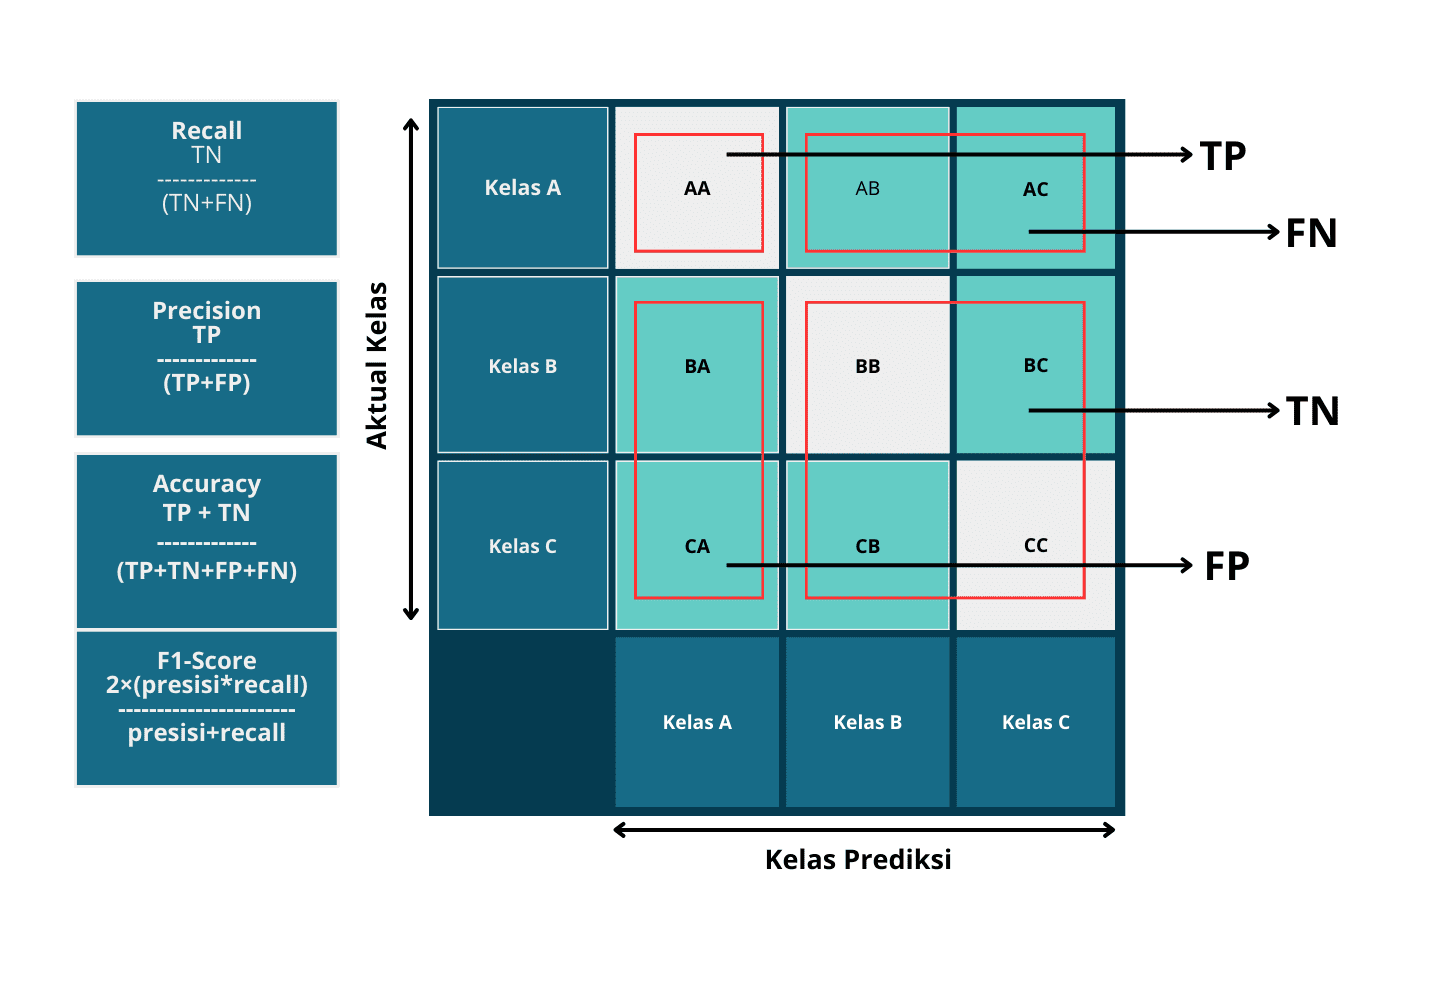
\includegraphics[width=0.75\textwidth]{figures/bab2/confusion matriks.png}
      \caption{\textit{Confusion Matrix}}
      \label{Confusion Matrix}
    
    \end{figure}

    Gambar 2.14 menampilkan empat nilai, yaitu "\textit{True Positive}" (TP), "\textit{False Negative}" (FN), "\textit{False Positive}" (FP), dan "\textit{True Negative}" (TN). Keempat nilai tersebut dapat digunakan untuk menghitung parameter-parameter seperti \textit{accuracy}, \textit{precision}, \textit{recall}, dan \textit{F1-Score} \cite{Nurhikmat2018}.

     \textit{Accuracy} digunakan untuk mengevaluasi sejauh mana model mampu melakukan klasifikasi dengan tepat dengan Persamaan \ref{Accuracy} berikut. 
     
    \begin{equation}
        \begin{aligned}
            \textit{Accuracy} = \frac{\text{TP} + \text{TN}}{\text{TP} + \text{TN} + \text{FN} + \text{FP}}
        \end{aligned}\label{Accuracy}
    \end{equation}


    \textit{Recall} merupakan parameter yang didapat dari jumlah data benar untuk mengukur seberapa baik model dalam mengidentifikasi kelas positif. \textit{Recall} juga dikenal sebagai sensitifitas prediksi dengan Persamaan \ref{Recall} beriikut.

    
    \begin{equation} 
        \begin{aligned}
            \textit{Recall} = \frac{\text{TP}}{\text{TP} + \text{FN}} 
        \end{aligned}\label{Recall}
    \end{equation}

    \textit{Precision} merupakan parameter penilaian yang menghitung jumlah data yang benar antara nilai sebenarnya dengan hasil prediksi model. Digunakan juga untuk mengukur seberapa baik model dalam mengidentifikasi kelas positif dengan menggunkan Persamaan \ref{Precision} berikut.
     \begin{equation}
        \begin{aligned}
            \text{\textit{Precision}} = \frac{\text{TP}}{\text{TP} + \text{FP}}
        \end{aligned}\label{Precision}
    \end{equation}

    \textit{F1-Score} merupakan rata-rata harmonik dari recall dan precision dengan Persamaan \ref{F1-Score}. Secara representasi, jika \textit{F1-Score} punya skor yang baik mengindikasikan bahwa model klasifikasi yang ada memiliki nilai \textit{recall} dan precision yang baik.

     \begin{equation}
        \begin{aligned}
         F1-Score =   2 \times \frac{precision \times recall}{precision + recall}
        \end{aligned}\label{F1-Score}
    \end{equation}

    


    


    \chapter{METODOLOGI PENELITIAN}

\section{Tempat dan Jadwal Kegiatan Penelitian}
    Penelitian ini telah dilaksanakan di Institut Teknologi Sumatera (ITERA), yang menjadi tempat utama melakukan analisis data  penelitian ini. Dengan fasilitas tersebut, peneliti dapat menjalankan eksperimen, mengakses sumber daya komputasi yang diperlukan, dan melakukan pengolahan data secara efisien. Informasi lebih lanjut mengenai jadwal kegiatan penelitian dapat ditemukan pada Gambar \ref{Jadwal Penelitian} berikut.

% \begin{figure}[H]
%     \centering
%     \scriptsize
%     \begin{ganttchart}[
%         y unit title=0.5cm,
%         y unit chart=0.5cm,
%         vgrid,
%         hgrid,
%         title label anchor/.style={below=-1.5ex},
%         title left shift=.05,
%         title right shift=-.05,
%         title height=1.1,
%         title label font=\small, % Ukuran font title
%         bar height=0.75, % Tinggi batang
%         group right shift=0,
%         group top shift=.5,
%         group height=.35,
%         bar/.style={fill=cyan!70, draw=none}, % Menghilangkan garis tepi batang
%         milestone/.append style={fill=orange!90, draw=none}, % Menghilangkan garis tepi milestone
%         milestone label font=\scriptsize, % Ukuran font milestone label
%         bar label font=\scriptsize, % Ukuran font batang label
%         ]{1}{23}
        
%         % labels
%         \gantttitle{Jadwal Penelitian}{23}\\ 
%         \gantttitle{2023}{10} 
%         \gantttitle{2024}{13}\\
%         \gantttitle{Sep}{2} 
%         \gantttitle{Okt}{3} 
%         \gantttitle{Nov}{3} 
%         \gantttitle{Des}{2} 
%         \gantttitle{Jan}{2} 
%         \gantttitle{Feb}{2}
%         \gantttitle{Mar}{2}
%         \gantttitle{Apr}{3}
%         \gantttitle{Mei}{2}
%         \gantttitle{Jun}{2}\\
        
%         % tasks
%         \textbf{\ganttbar{PROPOSAL TA}{1}{12}} \\
%         \ganttbar{Pengajuan Judul}{1}{2} \\
%         \ganttbar{Perencanaan}{3}{5} \\
%         \ganttbar{Penyusunan}{6}{10} \\
%         \ganttbar{Seminar Proposal}{11}{12} \\
%         \textbf{\ganttbar{HASIL TA}{12}{23}\ \\}
%         \ganttbar{Pengumpulan Data}{13}{13} \\
%         \ganttbar{Analisis Data}{14}{16}\\
%         \ganttbar{Seminar Hasil}{15}{17} \\
%         \ganttbar{Final TA}{18}{19} \\
%         \ganttbar{Sidang TA}{20}{23}
        
%         % relations 
%         \ganttlink{elem1}{elem2} 
%         \ganttlink{elem2}{elem3} 
%         \ganttlink{elem1}{elem2} 
%         \ganttlink{elem3}{elem4} 
%         \ganttlink{elem4}{elem6} 
%         \ganttlink{elem6}{elem7} 
%         \ganttlink{elem7}{elem8} 
%         \ganttlink{elem8}{elem9} 
%         \ganttlink{elem9}{elem10} 
%     \end{ganttchart}
%     \caption{Jadwal Penelitian}
%     \label{Jadwal Penelitian}
% \end{figure}








\section{Rancangan Penelitian}

   Penelitian ini dilakukan dengan tujuan untuk mengidentifikasi  masalah, yaitu mencari, mengumpulkan, dan mengidentifikasi isu-isu yang relevan. Setelah itu, mengevaluasi masalah yang diselesaikan dengan tindakan melakukan studi literatur dalam upaya mengidentifikasi solusi yang dapat diterapkan untuk masalah yang telah diidentifikasi dan ditetapkan sebelumnya, pendekatan yang digunakan adalah dengan membaca berbagai kutipan dari publikasi penelitian terkait, termasuk buku, jurnal, dan skripsi, tesis, dll. Diagram alir untuk penelitian ini terdiri dari beberapa tahap, yang masing-masing dijelaskan pada Gambar \ref{Diagram Alir Penelitian} berikut. 



    % \begin{figure}[H]
    %   \centering
    %   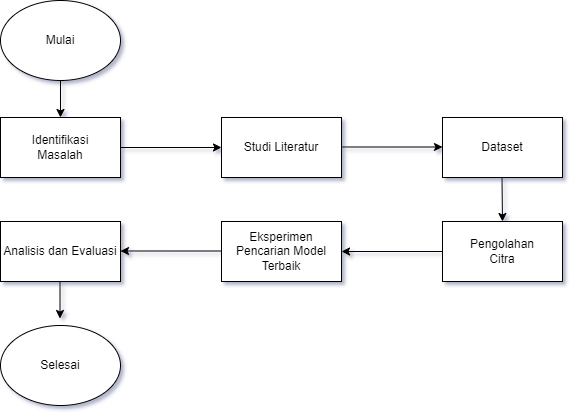
\includegraphics[width=0.8\textwidth]{figures/bab3/Diagram alir penelitian.png}
    %   \caption{Diagram Alir Penelitian}
    %   \label{Diagram Alir Penelitian}
    %   \medskip % spasi vertikal
    %   \begin{minipage}{0.8\textwidth}
    %     \centering
    %     %Sumber: \url{https://idanovinda.medium.com/mengapa-diperlukan-regularisasi-pada-model-neural-network-d622ed98f9a8}
    %   \end{minipage}
    % \end{figure}



    Data yang digunakan merupakan data sekunder dengan format video, oleh sebab itu peneliti tidak melakukan pengambilan data secara langsung. Data akan di ekstrak kedalam bentuk gambar, selanjut beralih ke pemrosesan citra, yang meliputi prapemrosesan dan penambahan data, eksperimen, analisis, dan penilaian. Proses yang akan dilakukan mencakup seluruh rentang dari  pengambilan dataset hingga penilaian dan analisis, semuanya diarahkan dengan tujuan membangun model yang efisien. 
    
    Proses klasifikasi secara umum dimulai dengan eksplorasi data video yang berfokus pada fitur-fitur video yang relevan. Tahap selanjutnya adalah praproses awal, yang meliputi seleksi fitur, penentuan nilai EAR (\textit{Eye Aspect Ratio}) dan MAR \textit{(Mouth Aspect Ratio}), dan konversi data video menjadi data gambar. Sebelum memasuki tahap klasifikasi menggunakan CNN \textit{(Convolutional Neural Network}), data terlebih dahulu menjalani praproses kedua, yaitu proses augmentasi data dan melakukan pembagian data menjadi data latih (\textit{training}) dan set data uji (\textit{testing}).

    Pada tahap klasifikasi, model akan menghasilkan metrik evaluasi seperti akurasi,\textit{ precision}, \textit{recall}, dan \textit{f1-score}. Hasil evaluasi ini kemudian dianalisis dan dievaluasi. Jika hasil evaluasi telah memenuhi kriteria yang ditetapkan, maka proses klasifikasi selesai. Namun, jika hasil evaluasi belum memenuhi kriteria, maka proses klasifikasi akan diulangi dengan kembali ke tahap praproses awal. Setiap tahap dalam proses klasifikasi digambarkan secara visual dalam Gambar \ref{flowchart}.


    % \begin{figure}[H]
    %   \centering
    %   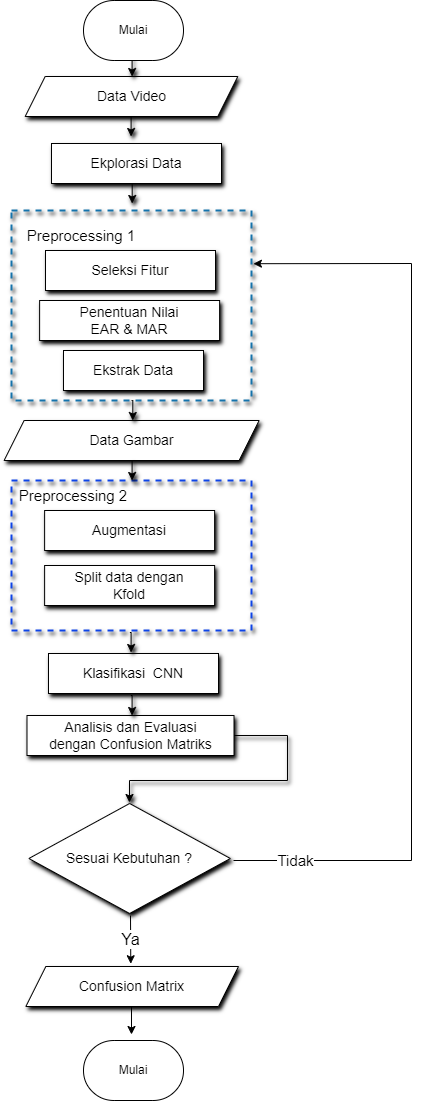
\includegraphics[width=0.6\textwidth]{figures/bab3/1flowchart.png}
    %   \caption{Gambaran Umum Sistem Klasifikasi}
    %   \label{flowchart}
    %   \medskip % spasi vertikal
    %   \begin{minipage}{0.8\textwidth}
    %     \centering

    %   \end{minipage}
    % \end{figure}


    

\section{Instrumen Penelitian}

Dalam penelitian ini, proses pelatihan CNN dilakukan dengan menggunakan layanan \textit{Google Colabboration}. Sementara untuk spesifikasi perangkat yang digunakan ditampilkan sebagai berikut.


    \begin{enumerate}
        \item Penelitian ini memanfaatkan perangkat lunak berikut:

        \begin{enumerate}
            \item \textit{Windows 11 x64}
            \item \textit{Python 3.11.4}
            \item \textit{Tensorflow 2.9.1}
            \item \textit{Conda 22.9.0} \item \textit {Dlib 19.22.1}
            \item \textit{Open CV 4.8.1}
            \item \textit{Google Colaboratory}
        \end{enumerate}
        
        \item Penelitian ini memanfaatkan perangkat keras berikut: laptop Lenovo dengan \textit{processor} AMD  A8-7410 \textit{with} AMD Radeon Graphics (4 CPUs),  2.2 GHz, RAM 12 GB DDR3L, dan SSD 256 GB.

    \end{enumerate}
    
\section{Penjabaran Langkah Penelitian}

    Untuk memperjelas setiap langkah-langkah yang telah didefinisikan pada Gambar \ref{Diagram Alir Penelitian}. Berikut ini akan dijabarkan secara rinci tahapan-tahapan yang dilakukan dalam penelitian ini.
    
\subsection{Studi literatur}

    Langkah awal penelitian ini melibatkan pengumplan literatur untuk menghimpun informasi, referensi, konsep dasar, dan pengetahuan yang menjadi dasar penelitian. Proses ini mencakup pencarian dan pembacaan berbagai sumber seperti buku, jurnal, dan artikel yang terkait dengan penelitian ini. Selain itu, dilakukan analisis menyeluruh terhadap penelitian-penelitian sebelumnya untuk memahami berbagai perkembangan penelitian dibidang yang sama.

    
\subsection{Data}

    Data yang dimanfaatkan dalam penelitian ini termasuk dalam kategori data sekunder dengan format video (avi). Sumber data ini berasal dari YAWDD: YAWNING DETECTION DATASET. Dataset ini mencakup pengemudi dengan berbagai karakteristik wajah yang digunakan untuk pengujian algoritma dan model untuk deteksi kantuk, tetapi juga pengenalan dan pelacakan wajah dan 
    mulut. Dalam kumpulan data ini, memberikan anotasi untuk properti-properti berikut (properti ditunjukkan dalam urutan berikut):


    \begin{enumerate}

        \item Video diambil dalam kondisi pencahayaan yang nyata dan bervariasi.
        \item Kamera dipasang di bawah kaca spion depan mobil dan \textit{dashboard} mobil. 
        \item  Setiap peserta memiliki tiga/empat video dan setiap video berisi kondisi mulut yang berbeda seperti normal berbicara/menyanyi, dan menguap. 
        \item Dataset ini menyediakan 316 video yang terdiri dari pengemudi pria dan 
        pengemudi pria dan wanita, dengan dan tanpa kacamata, dari etnis yang berbeda.
        \item Situasi: mengemudi normal (tidak berbicara), berbicara atau bernyanyi saat mengemudi, dan menguap menguap saat mengemudi.



    Contoh dataset yang digunakan ditampilkan pada Gambar \ref{Contoh Dataset} berikut.

    % \begin{figure}[H]
    %     \centering
    %     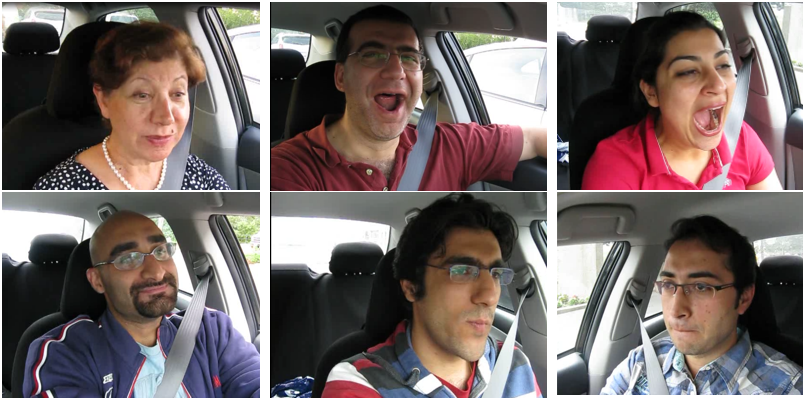
\includegraphics[width=0.85\textwidth]{figures/bab3/image.png}
    %     \caption{Contoh Dataset}
    %     \label{Contoh Dataset}
    % \end{figure}

        
    
    \end{enumerate}
    
  
    Setelah data dikumpulkan, proses selanjutnya melakukan pengolahan data, di mana video akan diklasifikasi dan diekstrak sesuai dengan kelasnya. Pra-pemrosesan data melibatkan sejumlah tugas, seperti penyesuaian ukuran dan pemotongan bingkai video, normalisasi data, serta ekstraksi fitur-fitur yang relevan dari konten video. Data kemudian dibagi menjadi \textit{subset} untuk keperluan pelatihan, validasi, dan pengujian model. Selain itu, data akan diterapkan pada arsitektur CNN untuk mendeteksi mengantuk pada pengemudi.
    
\subsection{\textit{Preprocessing }Data}
   
    Proses ini terkait dengan ekstraksi data, augmentasi data, pembagian data, ekstraksi fitur citra, dan klasifikasi citra. Tujuannya adalah untuk mencapai efisiensi yang baik dalam pelatihan model, baik dari segi akurasi maupun waktu, sehingga dapat meningkatkan kualitas dan kinerja model, serta memastikan keakuratan hasil.
    
  
\subsubsection{Ekstraksi Data}
    Penelitian ini menggunakan data berformat video (.avi) dengan ukuran 640 $x$ 480 piksel dengan resolusi 30 FPS. Sehingga perlu dilakukan  ekstrak video ke dalam bentuk gambar (.jpg). Eksraksi video ke gambar merupakan langkah penting dalam proses deteksi kantuk. Video diubah menjadi bingkai/gambar, kemudian dilakukan klasifikasi berdasarkan ekstraksi untuk daerah mata dan mulut. Penelitian ini menggunakan \textit{library} Dlib untuk detektor wajah dan 68 \textit{facial landmark predictors} untuk mata dan mulut. Proses ini melibatkan konversi setiap \textit{frame} video menjadi gambar langsung di kelompokkan berdasarkan kelasnya. Nilai EAR (\textit{Eye Aspect Ratio}) dan MAR \textit{(Mouth Aspect Ratio}) akan digunakan dalam klasifikasi pada setiap \textit{frame}.
    
    \begin{enumerate}
        \item     \textit{\textbf{Eye Aspect Ratio (EAR)}} digunakan untuk mengukur keterbukaan mata. EAR dihitung dengan menggunakan rasio jarak antara beberapa\textit{ landmark }mata. Nilai EAR berkisar antara 0 dan 1. Nilai EAR yang mendekati nol menunjukkan bahwa mata tertutup, sedangkan nilai EAR yang mendekati satu menunjukkan bahwa mata terbuka lebar

        \item \textbf{\textit{Mouth Aspect Ratio }}(MAR) digunakan untuk mengukur lebar bukaan mulut. MAR dihitung dengan menggunakan rasio jarak antara beberapa \textit{landmark} di sekitar mulut. Nilai MAR yang mendekati nol menunjukkan bahwa mulut tertutup rapat, sedangkan nilai MAR yang mendekati satu menunjukkan bahwa mulut terbuka lebar. 
    \end{enumerate}

    Untuk lebih jelasnya terkait ekstraksi video ke dalam bentuk foto dengan EAR dan MAR, akan ditampilkan ilustrasi pada Gambar \ref{Alur Ekstraksi Video} berikut.
    
  
    % \begin{figure}[H]
    %     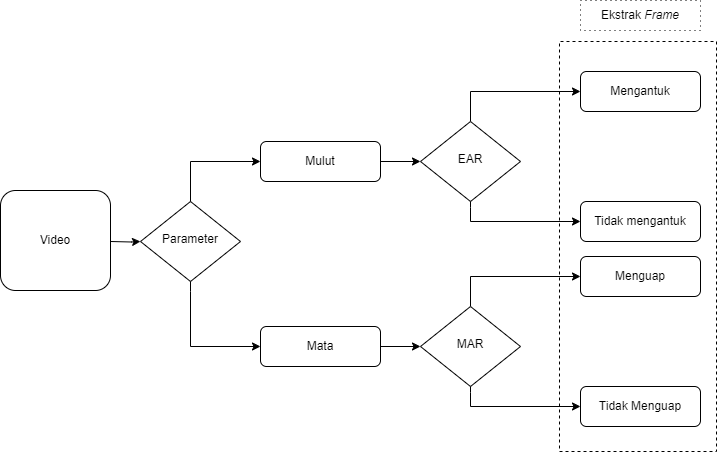
\includegraphics[width=1.0\textwidth]{figures/bab3/procesing.png}
    %     \caption{Alur Ekstraksi Video}
    %     \label{Alur Ekstraksi Video}
    % \end{figure}

    

    

    
    Setiap data yang diekstrak ke bentuk gambar akan dikelompokkan berdasarkan kelasnya, di mana setiap \textit{frame}nya akan dikelompokkan berdasarkan kelasnya. Kelas pada dataset digunakan berdasarkan kondisi mata dan mulut. Kedua parameter ini akan digunakan untuk mendeteksi kantuk. Mata yang terbuka ditandai dengan nilai EAR yang mengecil dan akan dikelompokkan pada kategori mengantuk untuk setiap \textit{frame}, sedangkan yang lainnya tidak mengantuk. Sementara itu, mulut digunakan untuk mengkategorikan keadaan menguap atau tidak. Nilai MAR yang semakin bertambah menandakan mulut terbuka dan dikategorikan sebagai menguap, sedangkan yang lainnya tidak menguap. Kombinasi dari kedua parameter tersebut akan menghasilkan beberapa kelas yang akan dilatih pada arsitektur CNN. Berikut ini adalah kategori kelas yang akan digunakan. Yang dapat dilihat pada Tabel \ref{Keterangan Anotasi Kelas} berikut.


    
    \begin{table}[h]
        \centering
        \caption{Keterangan Anotasi Kelas}
        \begin{tabular}{cccc}
            \hline
            \textbf{Kondisi Mata} & \textbf{Kondisi Mulut} & \textbf{Hasil} \\
            \midrule Mengantuk & Menguap &  Mengantuk dan Menguap\\
                     Mengantuk & Tidak Menguap &  Mengantuk tidak Menguap \\
                     Tidak Mengantuk & Menguap &  Menguap tidak Mengantuk\\
                
        
            \bottomrule
        \end{tabular}
        \label{Keterangan Anotasi Kelas}
    \end{table}
    

\subsubsection{Augmentasi Data}

    Setelah video di ekstraksi ke bentuk gambar, perlu dilakukan proses pengolahan citra dari data yang sebelumnya diperoleh. Proses augmentasi adalah teknik yang sering digunakan untuk meningkatkan ukuran kumpulan data tanpa memerlukan pengambilan data tambahan. Teknik ini melibatkan pengambilan data selama tahap pengumpulan dan persiapan data sebelumnya. Salah satu pendekatannya melibatkan penerapan transformasi pada data gambar asli. Transformasi ini dapat dilakukan berupa rotasi, pemberian \textit{noise}, penskalaan, pemotongan, dan penambahan nilai piksel melalui modifikasi kecerahan. Semuanya ini dilakukan untuk meningkatkan ukuran dan variasi data. Teknik ini dilakukan dengan tujuan untuk mengurangi resiko \textit{overfitting}.

\subsubsection{\textit{Splitting} Data}
   Data akan dipisahkan menjadi tiga kategori: data \textit{test}, data \textit{validation}, dan \textit{train}. Data \textit{train} ditujukan untuk memfasilitasi proses pembelajaran model selama fase pelatihan. Data \textit{validation} digunakan untuk memberikan informasi yang tidak bias kepada model. Selanjutnya, data ini secara konsisten digunakan selama percobaan, sehingga model sering terpapar dengan data tersebut. Hasil dari eksperimen yang dilakukan secara tidak langsung mempengaruhi model melalui data \textit{validation}. 
   Data pengujian digunakan untuk menilai kinerja model dengan data baru yang belum pernah dilihat, yang digunakan hanya sekali pada eksperimen. Pembagian ini diimplementasikan dengan tujuan untuk mencapai distribusi yang seimbang dan untuk mengoptimalkan kemampuan generalisasi model.

\subsection{Desain Arsitektur CNN}

    Merancang struktur yang efektif dengan mengekstrak fitur penting dari data gambar disebut sebagai desain arsitektur \textit{Convolutional Neural Network} (CNN). CNN adalah tipe arsitektur yang umum digunakan dalam pemrosesan gambar dan berbagai aplikasi pengenalan pola. Tujuan dari klasifikasi ini adalah untuk menghasilkan luaran yang menunjukkan keadaan pengendara sesuai dengan kelas yang telah di tetapkan. Seperti mengantuk dan menguap, mengantuk dan tidak menguap, menguap tidak mengantuk.  Proses diilustrasikan pada Gambar \ref{Proses Convolusional Neural Network} berikut.
 
    %  \begin{figure}[H]
    %   \centering
    %   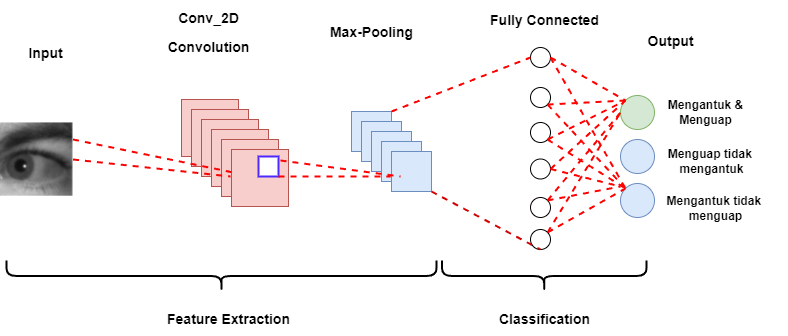
\includegraphics[width=0.85\textwidth]{figures/bab3/cnn_arsitektur.png}
    %   \caption{Proses \textit{Convolusional Neural Network}}
    %   \label{Proses Convolusional Neural Network}
    
    %   \medskip % spasi vertikal
    %   \begin{minipage}{0.8\textwidth}
    %     \centering

    %   \end{minipage}
    % \end{figure}

    Proses pelatihan menggunakan data berlabel yang telah dipisahkan ke dalam kumpulan data \textit{train}, \textit{test}, dan \textit{validation}. Kemudian akan dilakukan \textit{tuning hyperparameter} seperti \textit{activation layer}, \textit{learning rate} dan \textit{optimizer}. Augmentasi data dilakukan untuk memodifikasi data gambar sedemikian rupa sehingga, meskipun komputer menganggap gambar telah diubah sebagai gambar baru, manusia masih dapat mengenalinya sebagai gambar yang sama. Selanjutnya, hasil pemrosesan di evaluasi dan diuji pada tahap perbandingan model untuk menentukan model yang optimal untuk mengklasifikasikan dataset.

\subsection{\textit{Traning} Data}

    Setelah arsitektur CNN disesuaikan, penulis akan melatih model menggunakan data yang telah melalui tahap \textit{preprocessing}. Proses pelatihan melibatkan penyesuaian bobot dan \textit{bias} pada setiap lapisan CNN agar mampu mengenali citra dengan akurasi yang tinggi. Pada saat pelatihan di terapkan teknik \textit{early stopping} hal ini bertujuan untuk mencegah \textit{overfitting} dan mengoptimalkan waktu pelatihan. Teknik ini bekerja dengan menghentikan proses pelatihan lebih awal jika performa model pada data validasi tidak meningkat setelah sejumlah epoch tertentu.
    
    Untuk membuat model yang dapat mendeteksi kantuk serta dapat melakukan prediksi dengan efektif, dilakukan beberapa eksperimen yang saling berkaitan dan berhubungan satu sama lain.

     \begin{enumerate}
  
        \item Eksperimen Ke-1

        Eksperimen pertama dilakukan untuk menguji berbagai nilai atau jenis \textit{hyperparameter}. \textit{Hyperparameter} yang diuji adalah nilai atau jenis dari \textit{hyperparameter} yang digunakan dalam model. Model yang dihasilkan dari setiap kombinasi nilai atau jenis \textit{hyperparameter} kemudian dievaluasi untuk mengukur akurasi. \textit{Hyperparameter} yang menghasilkan model dengan akurasi paling optimal kemudian digunakan pada eksperimen selanjutnya. Rentang nilai atau jenis \textit{hyperparameter} yang diuji dapat dilihat pada Tabel \ref{Pengujian Parameter} berikut.



            \begin{table}[h]
            \centering
            \caption{Pengujian Parameter}
            \begin{tabular}{cccc}
                \toprule
                \textbf{} & \textbf{Parameter} \\
                \midrule
                      
                          \textit{Activation}  &  \textit{ReLu, Softmax, Sigmoid }\\
                         \textit{Optimizer} &  \textit{Adam, SGD} \\
                          \textit{Learning Rate} &  0.01, 0.001, 0.0001 \\
            
                \bottomrule
            \end{tabular}
            \label{Pengujian Parameter}
        \end{table}
        
        
        \item Eksperimen ke-2

        Eksperimen kedua merupakan eksperimen yang dilakukan untuk menguji performa model dengan menggunakan arsitektur CNN dan \textit{hyperparameter} yang telah dioptimalkan. Model yang digunakan pada eksperimen ini adalah model yang dihasilkan dari eksperimen sebelumnya. Data uji digunakan untuk mengevaluasi performa model dalam memprediksi data yang belum pernah dilihat sebelumnya.

        
       
    \end{enumerate}




 

\section{Evaluasi Hasil}

    Dalam penelitian ini, kinerja pengenalan atau klasifikasi diukur dengan menggunakan teknik yang telah banyak diterapkan dalam skenario penelitian serupa. Selain itu, pendekatan \textit{confusion matrix} juga diterapkan, seperti yang terlihat pada Gambar \ref{Confusion Matrix}, karena data yang digunakan adalah data berlabel. Pada tahap ini, Peneliti mengukur performa model CNN menggunakan \textit{confusion matrix} yang mencakup \textit{accuracy}, \textit{recall},\textit{ precision}, dan \textit{f-1 score}.

    \textit{True Positive} (TP) menunjukkan jumlah gambar pengemudi yang mengantuk yang diidentifikasi dengan benar oleh model. Hal ini terjadi ketika model secara akurat menilai gambar pengemudi yang disediakan. Sebaliknya, \textit{False Positive} (FP) adalah jumlah data yang salah yang diklasifikasikan sebagai benar. \textit{False Negative} (FN) menunjukkan jumlah data yang benar yang salah diklasifikasikan sebagai salah. Hal ini terjadi ketika model gagal untuk secara akurat menilai gambar yang diberikan tentang pengemudi yang mengantuk, sehingga menghasilkan output yang tidak sesuai dengan input yang diberikan. Terakhir, \textit{True Negative} (TN) menunjukkan jumlah data yang sebenarnya salah yang berhasil diklasifikasikan oleh model.
    
    Keempat kriteria penilaian dalam \textit{confusion matrix }penelitian ini didasarkan pada kemampuan model dalam menilai setiap gambar berkendara yang telah diberi label sebelumnya. Semua prosedur eksperimental yang berhasil merupakan titik fokus utama dalam penyelidikan ini. Hasil dari setiap percobaan dibandingkan secara komprehensif untuk menyimpulkan analisis. Setiap eksperimen diteliti dan dinilai dengan cermat untuk menentukan potensinya dalam mencapai performa model tertinggi.



    % 
\chapter{HASIL DAN PEMBAHASAN}

\section{Ekplorasi Dataset}

    Penelitian ini menggunakan data video dalam format video (.avi). Jumlah data berjumlah 319 video yang terdiri dari 
    pengemudi pria berjmlah 163 video dan wanita berjumlah 156 video dengan resolusi 640 x 480 piksel dan kecepatan tiga 
    puluh \textit{frame per second} (FPS). Dataset ini memiliki beberapa penjelesan terkait dengan kondisi video, yaitu:
    
    \begin{enumerate}
        \item \textit{Participant Number}: Variabel yang memberikan informasi terkait dengan nomor partisipasi dalam dataset.
        \item \textit{Action}: Memberikan informasi terkait hal yang terjadi pada pengemudi.
        \item \textit{Scarf}:  Memberikan informasi apakah pengendara menggunakan syal atau tidak.
        \item \textit{Background Movement}: Memberitahukan kondisi latar belakang video, bergerak atau tidak.

         \item  \textit{Glasses}: Jenis kacamata yang digunakan.
        
        \item \textit{Lighting}: Memberikan informasi kondisi pencahayaan.
        
        \item  \textit{Ethnicity}: Jenis etnis pengendara.

        \item  \textit{Duration}: Durasi video pengendara dengan satuan detik
        
        
    \end{enumerate}


    Penjelesan dataset untuk setiap videonya disajikan dalam Tabel \ref{Penjelasan Dataset} berikut.

    \vspace{1cm}

  \begin{table}[htbp]
        \centering
        \caption{Penjelasan Dataset}
        \label{Penjelasan Dataset}
    \scriptsize
        \begin{tabular}{p{0.5cm} p{1.2 cm} p{1.2 cm} p{1.1cm} p{1.3 cm} {0.5 cm} {1.0 cm} {0.5 cm}{0.7cm}{0.6cm} }
        \hline
        \textbf{No.} & \textbf{Participant Number} & \textbf{Action} & \textbf{Scarf} & \textbf{BG Movement} & \textbf{Glasses} & \textbf{Lighting} & \textbf{Ethnicity} & \textbf{Durasi} \\
        \hline

        \hline
        1 & 1 & Talking & No & No & No Glasses & Sunny & Caucasian & 24 s\\
        2 & 1 & Yawning & No & No & Sun glasses & Sunny & Caucasian & 14 s\\
        3 & 1 & Normal & No & Yes & Prescription & Sunny & Middle Eastern & 16 s\\
        4 & 1 & Yawning & No & No & Prescription & Sunny & Caucasian & 14 s\\
        5 & 2 & Yawning & No & Yes & No Glasses & Sunny & Caucasian & 15 s \\
        6 & 2 & Talking & No & No & No Glasses & Sunny & Caucasian & 18 s\\
        7 & 2 & Yawning & No & No & Sun glasses & Sunny & Caucasian  & 14 s\\
        8 & 3 & Normal & No & Yes & Prescription & Sunny & Middle Eastern & 15 s\\
        ... &... & ... & ... & ... & ... & ... & ...& ...  \\
        ... &... & ... & ... & ... & ... & ... & ... & ... \\
        ... &... & ... & ... & ... & ... & ... & ... & ...  \\
        156 &142 & Yawning & No & No & No Glasses & Sunny & Middle Eastern & 22 s\\
        157 & 145 & Yawning & No & No & No Glasses & Sunny & Middle Eastern & 20 s\\
        158 &148 & Yawning & No & Yes & No Glasses & Sunny & Caucasian  & 16 s\\
        159 &151 & Yawning & No & No & No Glasses & Sunny & Caucasian& 19 s \\
        160 &154 & Yawning & No & Yes & No Glasses & Sunny & Middle Eastern & 23 s\\
        161 &157 & Yawning & No & Yes & No Glasses & Sunny & Middle Eastern & 37 s\\
        162 &160 & Yawning & No & Yes & Prescription & Sunny & Middle Eastern & 18 s\\
        \hline
        \end{tabular}
        \end{table}

    Contoh dataset awal yang berupa video ditampilkan seperti Gambar \ref{Dataset Video} berikut.

     \begin{figure}[H]
         \centering
             \centering
             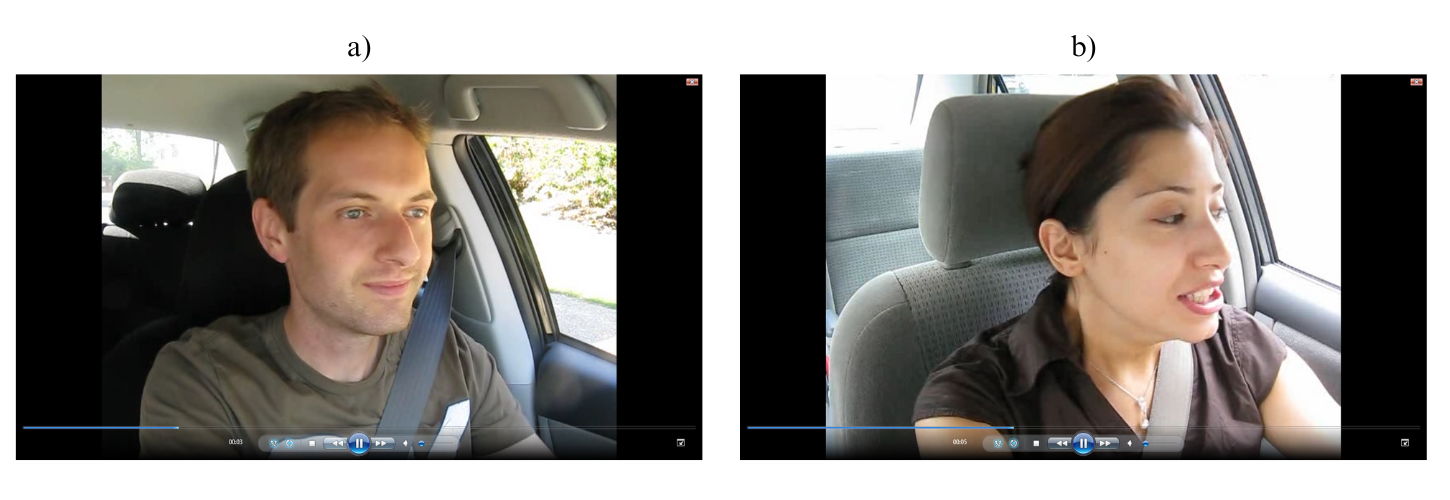
\includegraphics[width=\textwidth]{figures/bab4/data video.png}
             \caption{a) \textit{Male}, b) \textit{Female}}
             \label{Dataset Video}
     \end{figure}


    Data video diekstrak menjadi gambar dengan menggunakan nilai EAR dan MAR, setiap foto hasil ektraksi akan langsung otomatis masuk dalam folder sesuai dengan kelas yang telah ditentukan. Penentuan kelas sebuah gambar dikelompokkan pada kategori kelas tetentu di peroleh berdasarkan kondisi nilai EAR dan MAR seperti yang tertulis sebagai berikut.

    \begin{enumerate}
        \item    Jika nilai EAR pada \textit{frame} tersebut lebih kecil dari EAR \textit{threshold} dan MAR lebih besar MAR \textit{threshold} foto akan masuk dalam folder "mengantuk \& menguap".

        \item Jika nilai EAR pada \textit{frame} tersebut lebih kecil dari EAR \textit{threshold} dan MAR lebih kecil
    dari MAR \textit{threshold} foto akan masuk dalam folder "mengantuk \& tidak menguap "


     \item  Jika nilai EAR pada \textit{frame} tersebut lebih besar dari EAR \textit{threshold} dan MAR lebih besar
    dari MAR \textit{threshold} foto akan masuk dalam folder "menguap \& tidak mengantuk"


    \end{enumerate}

Nilai \textit{threshold} yang dimaksut merupakan nilai ambang batas  yang menentukan gambar tersebut masuk 
dalam kategori mengantuk dan menguap, untuk lebih jelasnya akan dijelaskan pada bagian selanjutnya.
     

    

\section{Data \textit{Preprocessing}}

\subsection{\textit{Seleksi Fitur}}

    
   Sebelum memasuki tahap selanjutnya, data akan memasuki seleksi fitur. Hal ini bertujuan untuk mereduksi data atau 
   fitur yang tidak dibutuhkan. Pemilihan data dilakukan dengan memfilter data sesuai dengan deskripsi data setiap 
   video yang telah diberikan sebelumnya seperti pada Tabel \ref{Penjelasan Dataset}. Data dipisahkan secara manual 
   berdasarkan penamaan video pada setiap folder seperti Gambar \ref{Seleksi_Fitur} berikut.




     \begin{figure}[H]
         \centering
             \centering
             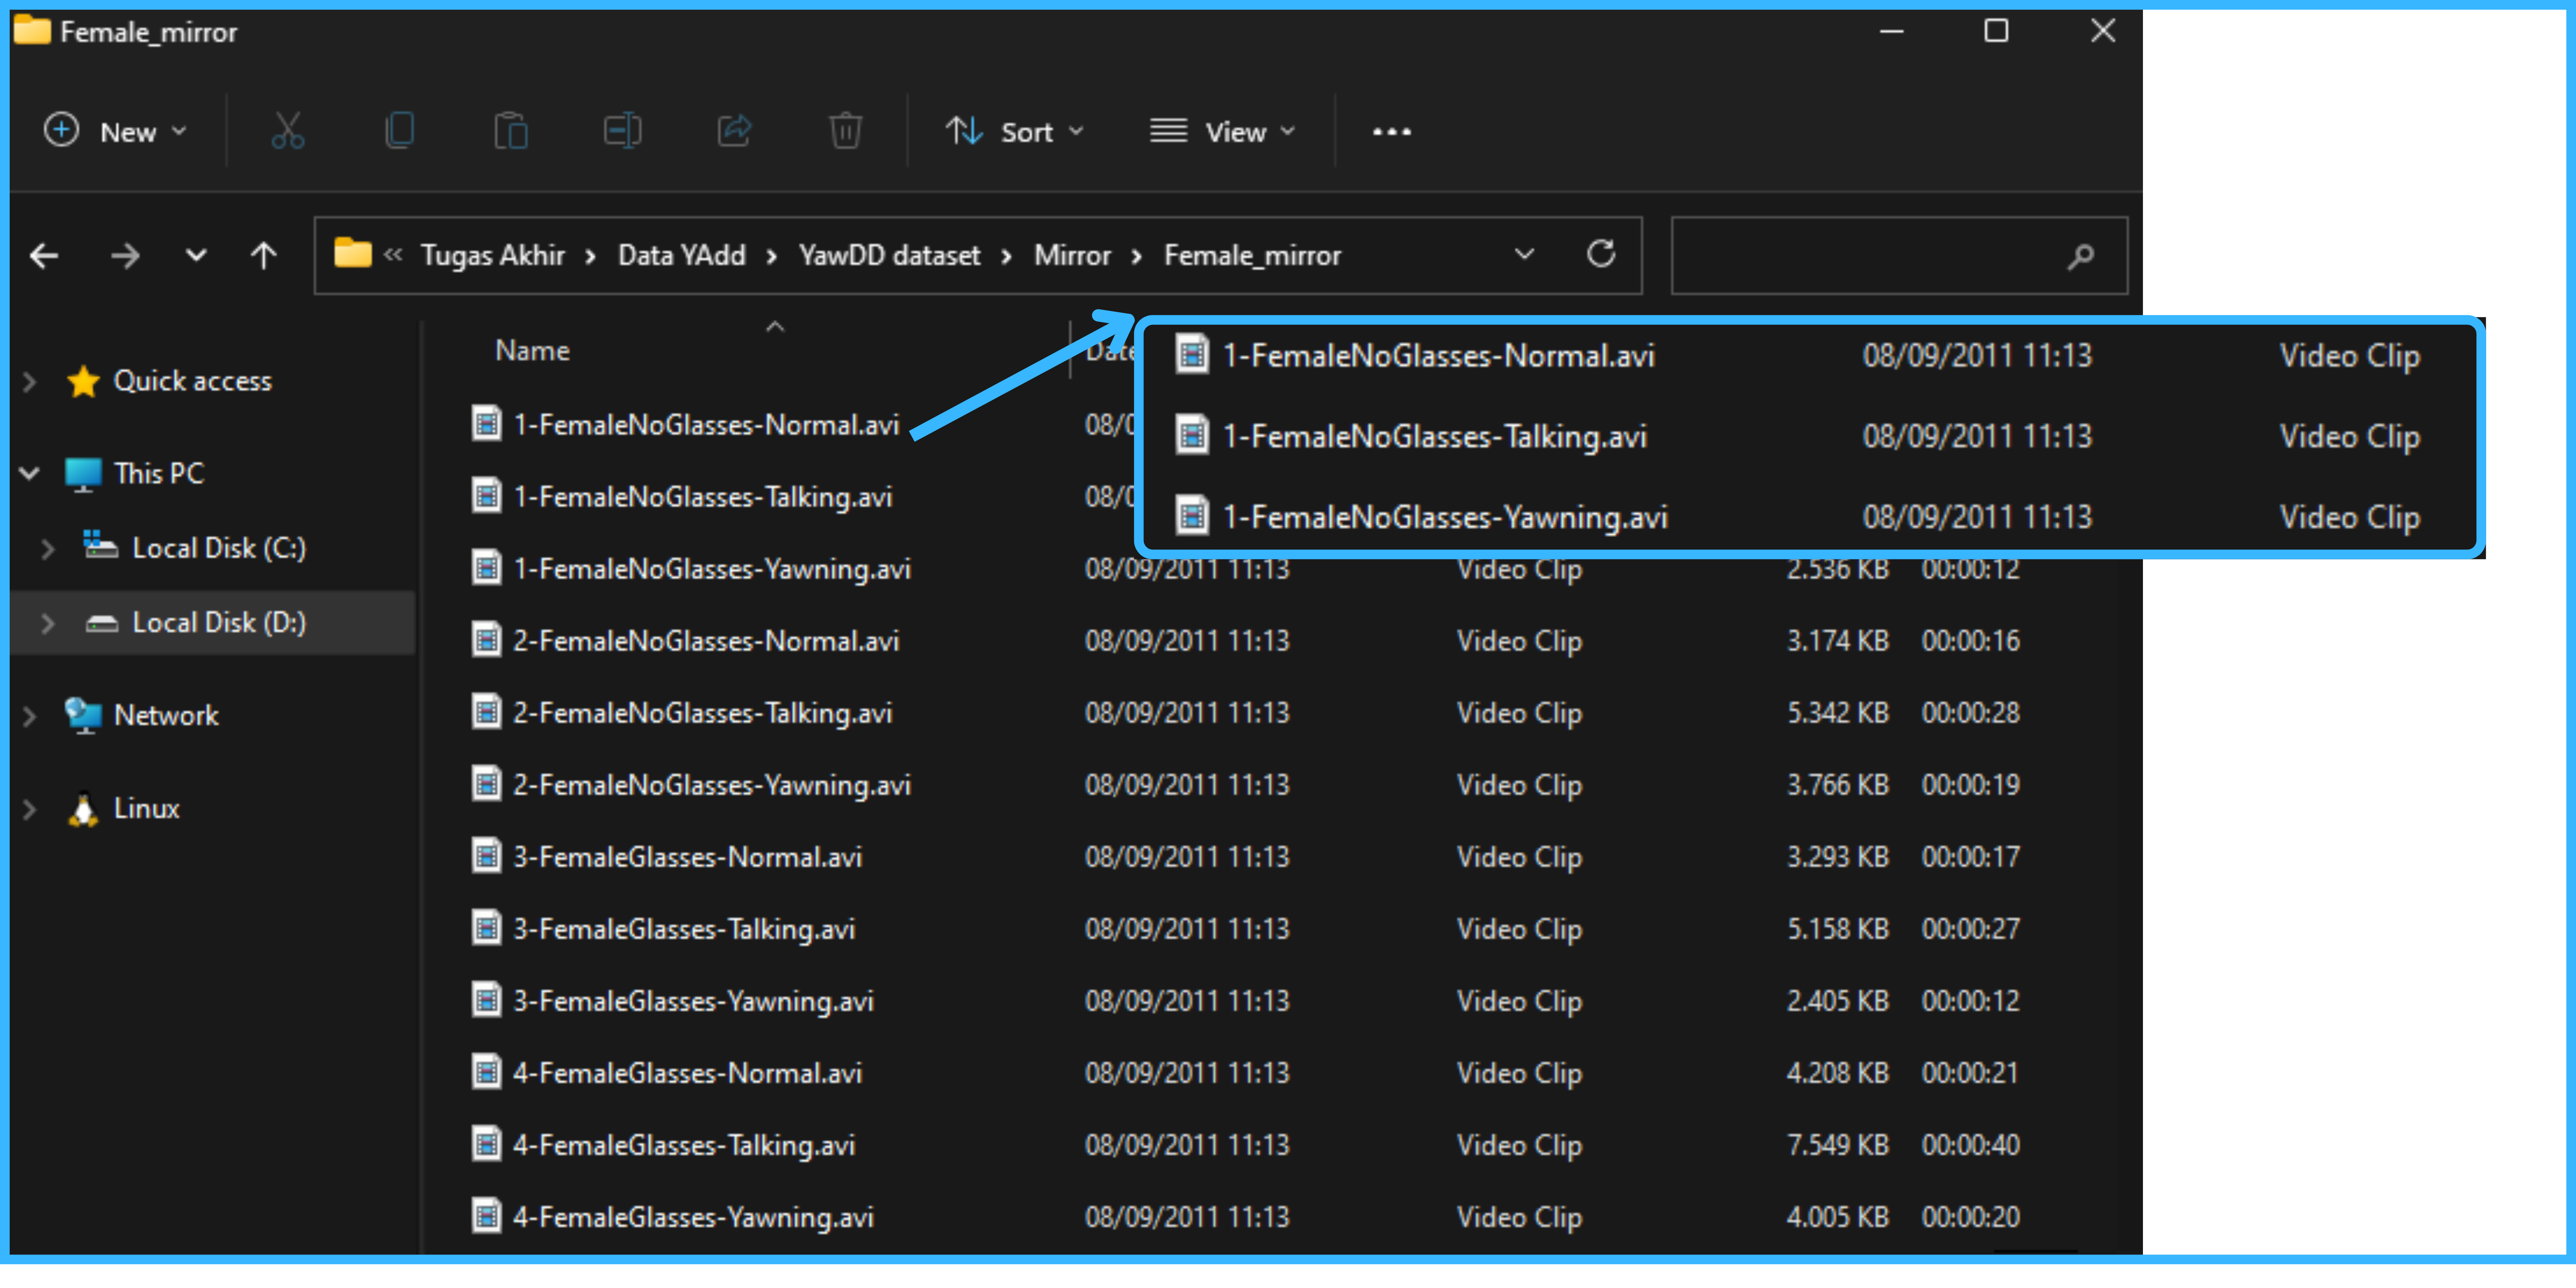
\includegraphics[width=\textwidth]{figures/bab4/seleksi_fitur.png}
             \caption{Seleksi Fitur}
             \label{Seleksi_Fitur}
     \end{figure}

     Penelitian ini berfokus pada analisis fitur \textit{"action"} untuk mendeteksi rasa kantuk pada pengemudi. 
     Dari berbagai fitur \textit{"action"}, hanya dua keadaan yang dipilih, yaitu \textit{"yawning"} (menguap) dan
     \textit{"yawning \& talking"} (menguap dan berbicara). Pemilihan ini didasarkan pada fokus penelitian pada
       pengemudi yang menunjukkan tanda-tanda kantuk, seperti menguap. Data dikumpulkan dalam format 
       gambar (.jpg) dan kemudian dilatih menggunakan model \textit{Convolutional Neural Network} (CNN). 
       Proses seleksi data dilakukan berdasarkan dua kategori, yaitu \textit{"male"} (laki-laki) dan \textit{"female"}
        (perempuan).
   


\subsubsection{\textit{Male}}
          Sebelum proses seleksi data, dilakukan eksplorasi data awal terkait fitur-fitur pada data. Hal ini bertujuan untuk memahami karakteristik data dan meninjau kembali kelayakan fitur-fitur yang telah dipilih. Contoh data dengan kategori \textit{'male}' ditampilkan pada Gambar \ref{male gambar1} berikut.
       
     \begin{figure}[H]
         \centering
             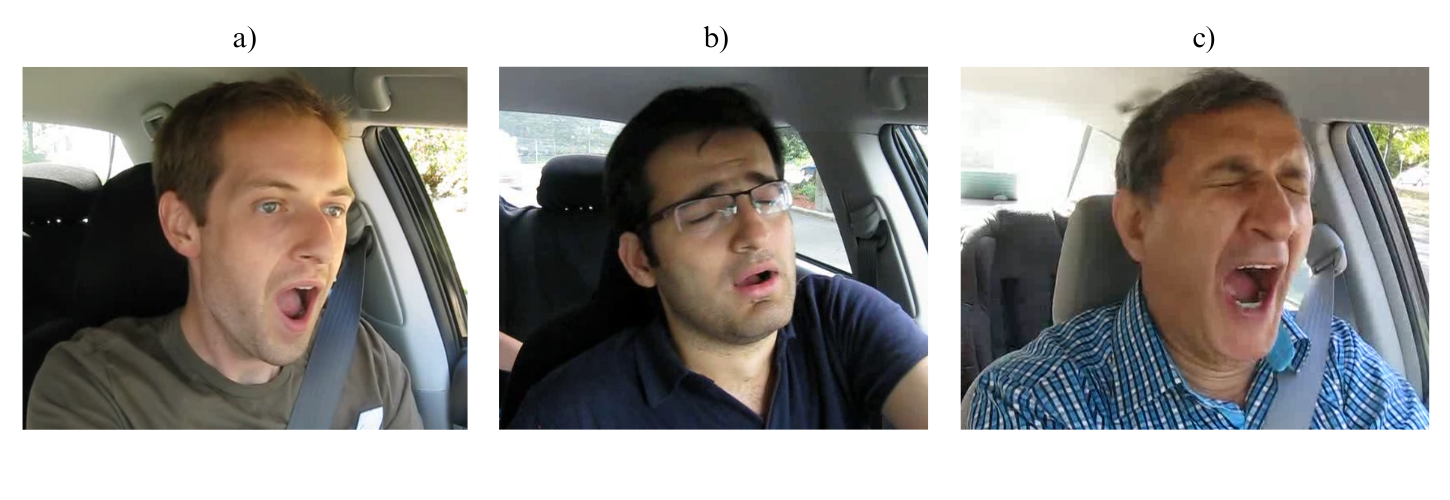
\includegraphics[width=\textwidth]{figures/bab4/male_contoh.png}
             \caption{Penampilan Data \textit{Male}}
             \label{male gambar1}
     \end{figure}

    Pada kategori data \textit{male} terdapat total 163 video (.avi). Berdasarkan deskripsi data pada fitur \textit{"action"} mencakup kondisi seperti \textit{"talking"}, \textit{"yawning"}, \textit{"normal"} dan \textit{"yawning \& talking"}. Proporsi data berdasarkan fitur \textit{action} pada kategori \textit{male} ditamilkan pada Gambar \ref{Proporsi Data Male Berdasarkan "Action"} berikut.
    

   

     \begin{figure}[H]
             \centering
         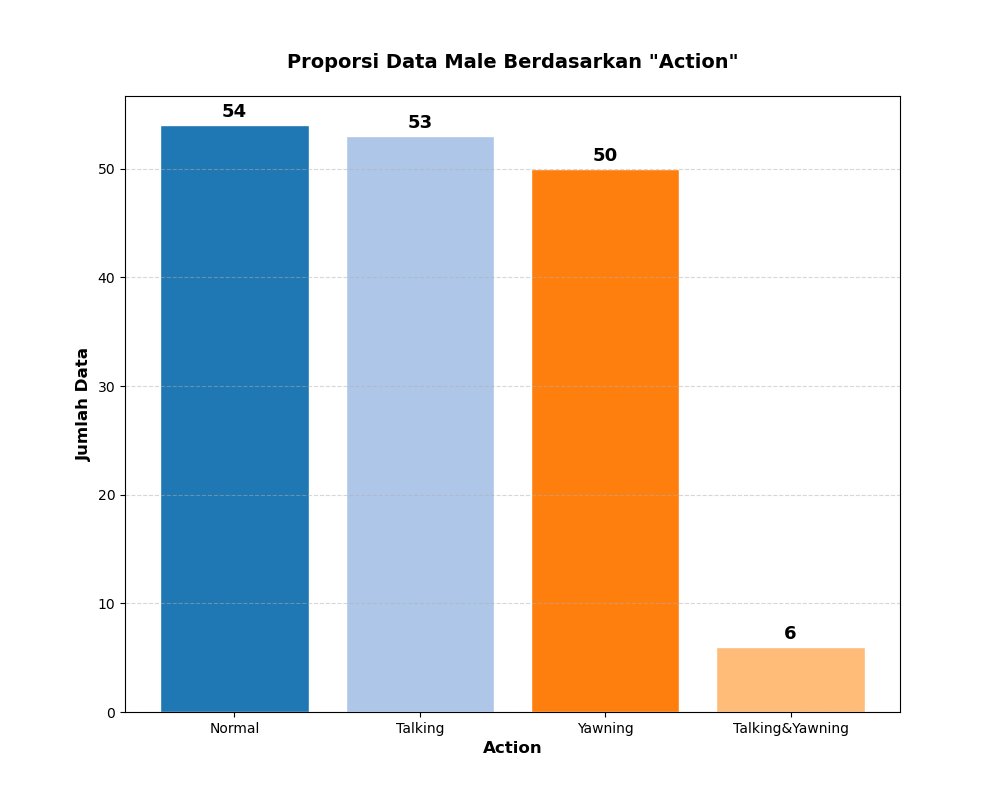
\includegraphics[width=0.75\linewidth]{figures/bab4/data_male.png}
         \caption{Proporsi Data \textit{Male} Berdasarkan \textit{"Action"}}
         \label{Proporsi Data Male Berdasarkan "Action"}
     \end{figure}

  


    Setelah dilakukan pemilihan fitur, di hasilkan jumlah data 
    untuk kategori \textit{male} sebanyak 56 video. Deskripsi untuk setiap data setelah sudah dilakukan pemilihan fitur untuk kategori \textit{male} ditampilkan pada Tabel \ref{Data male setelah dilakukan pemilihan fitur} berikut.

 
    \begin{table}[H]
        \centering
        \caption{Data \textit{Male} Setelah Dilakukan Pemilihan Fitur}
        \label{Data male setelah dilakukan pemilihan fitur}
        \scriptsize
        \begin{tabular}{p{0.2cm}p{1.2 cm}p{1.5cm}p{1.0cm}{0.5cm}{1.0 cm}{0.8 cm}{0.6cm}}
            \hline
            \textbf{No.} & \textbf{Participant Number} & \textbf{Action} & \textbf{Facial Hair} & \textbf{BG Movement} & \textbf{Glasses} & \textbf{Lighting} & \textbf{Ethnicity}\\
            \hline
            1 & 1 & Yawning & No & No & No Glasses & Sunny & Caucasian \\
            2 & 1 & Yawning & No & No & Sun glasses & Sunny & Caucasian \\
            3 & 2 & Yawning & No & Yes & Prescription & Sunny & Middle Eastern \\
            4 & 3 & Yawning & No & No & Prescription & Sunny & Caucasian  \\
            5 & 3 & Yawning & No & Yes & No Glasses & Sunny & Caucasian  \\
            6 & 4 & Yawning & No & No & No Glasses & Sunny & Middle Eastern  \\
            7 & 5 & Yawning & No & No & Sun glasses & Sunny & Middle Eastern  \\
            8 & 6 & Yawning & No & No & No Glasses & Sunny & Middle Eastern  \\
            9 & 7 & Yawning & No & No & Prescription & Sunny & Middle Eastern  \\
            10 & 8 & Yawning & Beard & Yes & Prescription & Sunny & Middle Eastern  \\
            11 & 9 & Yawning & No & No & No Glasses & Sunny & Caucasian \\
            12 & 10 & Yawning & No & No & No Glasses & Sunny & Middle Eastern  \\
            13 & 11 & Yawning & No & No & Prescription & Sunny & Middle Eastern \\
            14 & 12 & Talking \& Yawning & No & Yes & Prescription & Sunny & Middle Eastern  \\
            15 & 13 & Yawning & Beard & Yes & Prescription & Rainy & African  \\
            16 & 15 & Yawning & Beard & No & No Glasses & Rainy & African \\
            17 & 17 & Yawning & No & No & No Glasses & Sunny & Middle Eastern \\
            18 & 18 & Yawning & No & No & No Glasses & Sunny & Middle Eastern \\
            19 & 19 & Yawning & Moustache & No & Prescription & Sunny & Middle Eastern \\
            20 & 20 & Talking \& Yawning & No & No & Prescription & Sunny & Middle Eastern \\
            21 & 21 & Yawning & No & No & Prescription & Sunny & Middle Eastern \\
            22 & 22 & Yawning & Moustache & No & Prescription & Sunny & Middle Eastern \\
            23 & 23 & Talking \& Yawning & Beard & No & Prescription & Sunny & Middle Eastern  \\
            24 & 23 & Yawning & Beard & No & Prescription & Sunny & Middle Eastern  \\
            25 & 23 & Yawning & No & No & No Glasses & Sunny & Middle Eastern  \\
            26 & 24 & Yawning & No & No & Prescription & Cloudy & Middle Eastern \\
            27 & 25 & Yawning & Beard & No & Prescription & Cloudy & Middle Eastern  \\
            28 & 25 & Yawning & Beard & No & Sun glasses & Cloudy & Middle Eastern  \\
            29 & 26 & Yawning & No & Yes & No Glasses & Sunny & Middle Eastern \\
            30 & 27 & Yawning & No & No & Prescription & Sunny & Middle Eastern  \\
            31 & 27 & Yawning & No & No & No Glasses & Sunny & Middle Eastern  \\
            32 & 28 & Yawning & No & No & Prescription & Cloudy & Middle Eastern \\
            33 & 28 & Yawning & No & No & No Glasses & Cloudy & Middle Eastern \\
            34 & 29 & Yawning & No & Yes & No Glasses & Sunny & Caucasian  \\
            35 & 30 & Talking \& Yawning & No & Yes & Prescription & Sunny & Middle Eastern \\
            36 & 30 & Yawning & No & Yes & Prescription & Sunny & Middle Eastern  \\
            37 & 31 & Yawning & Beard & No & Prescription & Sunny & Middle Eastern  \\
            38 & 32 & Talking \& Yawning & No & Yes & Prescription & Cloudy & Middle Eastern \\
            39 & 32 & Yawning & No & No & Prescription & Cloudy & Middle Eastern \\
            40 & 33 & Talking \& Yawning & No & Yes & Prescription & Sunny & Middle Eastern \\
            41 & 33 & Yawning & No & No & Prescription & Sunny & Middle Eastern  \\
            42 & 34 & Yawning & No & Yes & No Glasses & Sunny & Caucasian \\
            43 & 35 & Yawning & No & No & No Glasses & Sunny & Middle Eastern \\
            44 & 36 & Yawning & No & Yes & No Glasses & Sunny & Caucasian  \\
            45 & 36 & Yawning & No & No & Sun glasses & Sunny & Caucasian \\
            46 & 37 & Yawning & Beard & Yes & No Glasses & Sunny & African  \\
            47 & 38 & Yawning & Beard & No & No Glasses & Sunny & African  \\
            48 & 38 & Yawning & Beard & Yes & Sun glasses & Sunny & African \\
            49 & 39 & Yawning & No & No & Prescription & Sunny & Asian & No \\
            50 & 40 & Yawning & No & No & No Glasses & Sunny & Middle Eastern  \\
            51 & 41 & Yawning & No & No & No Glasses & Sunny & Middle Eastern  \\
            52 & 42 & Yawning & No & No & No Glasses & Sunny & Middle Eastern  \\
            53 & 43 & Yawning & No & No & No Glasses & Sunny & Caucasian \\
            54 & 44 & Yawning & No & Yes & No Glasses & Sunny & Middle Eastern \\
            55 & 45 & Yawning & No & Yes & No Glasses & Sunny & Middle Eastern \\
            56 & 46 & Yawning & No & Yes & Prescription & Sunny & Middle Eastern \\
            \hline
        \end{tabular}
    \end{table}




\subsubsection{\textit{Female}}

    
    Pada kategori \textit{female} ditampilkan beberapa contoh data dengan kategori "\textit{female}" pada Gambar \ref{Female Dataset} berikut.
    
     \begin{figure}[H]
         \centering
         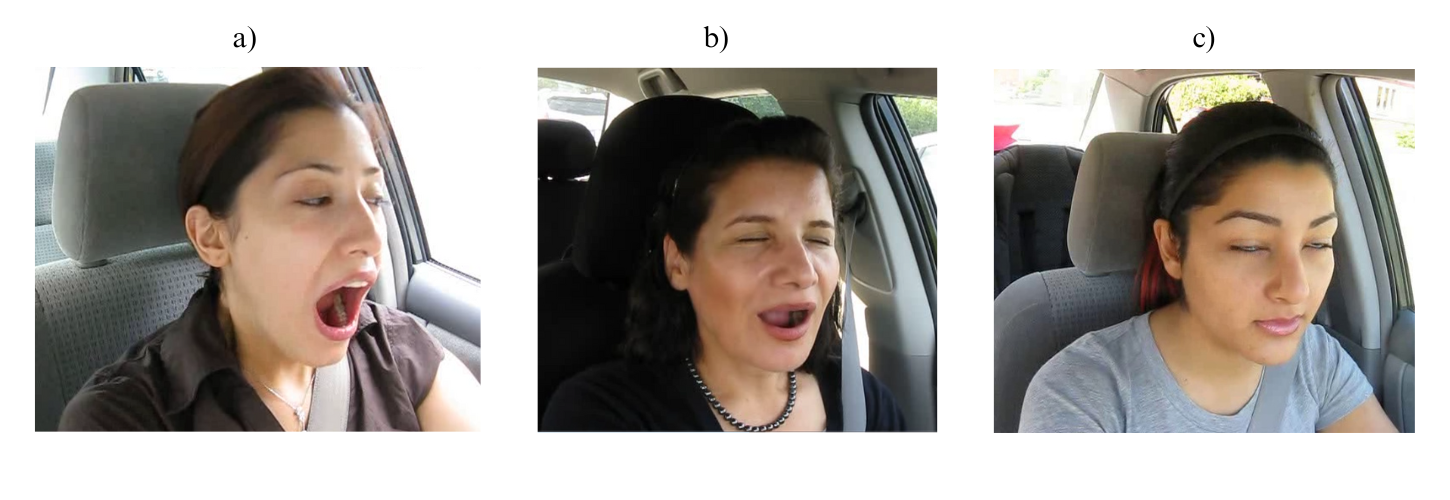
\includegraphics[width=1.0\linewidth]{figures/bab4/female_contoh.png}
         \caption{Contoh Data \textit{Female}}
         \label{Female Dataset}
     \end{figure}

   

     Terdapat 156 video pada kategori \textit{"female"}, fitur \textit{action} pada data mencakup keadaan \textit{"yawning"}, \textit{"talking"},\textit{"normal"} dan \textit{"yawning \& talking"}. Berikut proprosi untuk kategori \textit{action} di tampilkan pada Gambar \ref{Proporsi Data Female Berdasarkan "Action"} berikut.

     \begin{figure}[H]
         \centering
         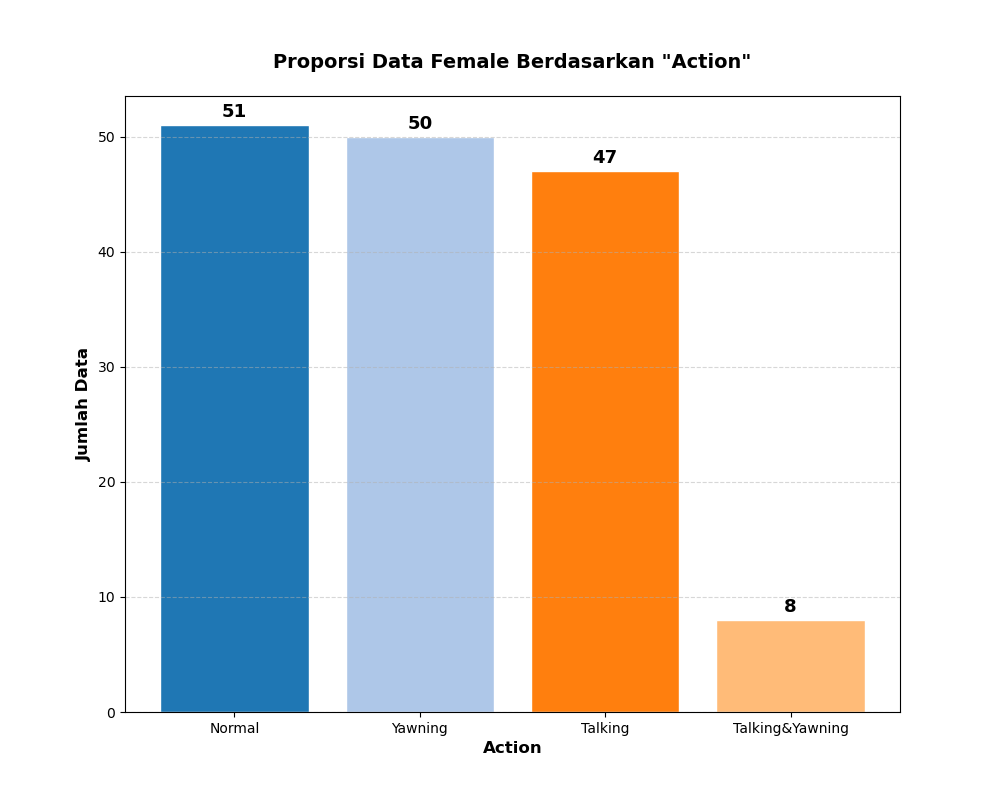
\includegraphics[width=0.75\linewidth]{figures/bab4/data_female.png}
         \caption{Proporsi Data \textit{Female }Berdasarkan \textit{"Action"}}
         \label{Proporsi Data Female Berdasarkan "Action"}
     \end{figure}

        Setelah dilakukan pemilihan fitur berdasarkan kolom 
        \textit{action}, yaitu hanya keadaan \textit{"yawning"} dan
         \textit{"talking \& yawning"} yang dipilih. Dihasilkan 
         jumlah data untuk kategori \textit{female} sebanyak 58 video. 
         Data \textit{female} setelah dilakukan pemilihan fitur 
         ditampilkan pada Tabel \ref{Data female setelah dilakukan pemilihan fitur} berikut.

        \begin{table}[H]
\centering
\caption{Data \textit{Female} Setelah Dilakukan Pemilihan Fitur}
\label{Data female setelah dilakukan pemilihan fitur}
\scriptsize

    \begin{tabular}{p{0.2cm}p{1.2 cm}p{1.5cm}p{1.0cm}{0.5cm}{1.0 cm}{0.8 cm}{0.6cm}}
    
    \hline
    \textbf{No.} & \textbf{Participant Number} & \textbf{Action} & \textbf{Scarf} & \textbf{BG Movement} & \textbf{Glasses} & \textbf{Lighting} & \textbf{Ethnicity} \\
    \hline
    1 & 2 & Yawning & No & No & No Glasses & Sunny & Middle Eastern \\
    2 & 5 & Yawning & No & No & No Glasses & Sunny & Middle Eastern  \\
    3 & 8 & Yawning & No & No & Prescription & Rainy & Caucasian  \\
    4 & 11 & Yawning & No & No & Prescription & Rainy & Caucasian \\
    5 & 14 & Yawning & No & No & Prescription & Rainy & Caucasian\\
    6 & 17 & Yawning & No & No & No Glasses & Rainy & Middle Eastern  \\
    7 & 20 & Yawning & No & No & Prescription & Cloudy & Middle Eastern \\
    8 & 23 & Yawning & No & No & Prescription & Cloudy & Middle Eastern  \\
    9 & 26 & Yawning & No & No & No Glasses & Cloudy & Middle Eastern \\
    10 & 29 & Yawning & No & No & No Glasses & Cloudy & Middle Eastern  \\
    11 & 32 & Yawning & No & Yes & No Glasses & Cloudy & Middle Eastern  \\
    12 & 35 & Yawning & No & Yes & No Glasses & Rainy & Middle Eastern \\
    13 & 38 & Talking \& Yawning & No & Yes & No Glasses & Sunny & Caucasian \\
    14 & 41 & Yawning & No & No & No Glasses & Sunny & Middle Eastern \\
    15 & 44 & Yawning & No & No & Prescription & Sunny & Middle Eastern  \\
    16 & 46 & Yawning & No & No & Sun glasses & Sunny & Middle Eastern  \\
    17 & 49 & Yawning & No & No & Prescription & Sunny & Middle Eastern \\
    18 & 52 & Yawning & No & No & No Glasses & Sunny & Middle Eastern \\
    19 & 55 & Yawning & No & No & Sun Glasses & Sunny & Middle Eastern  \\
    20 & 58 & Yawning & No & No & No Glasses & Sunny & Middle Eastern \\
    21 & 61 & Talking \& Yawning & No & No & Sun Glasses & Sunny & Middle Eastern  \\
    22 & 64 & Talking & No & No & No Glasses & Sunny & Middle Eastern  \\
    23 & 65 & Yawning & No & Yes & No Glasses & Sunny & Middle Eastern  \\
    24 & 68 & Yawning & No & Yes & No Glasses & Sunny & Middle Eastern \\
    25 & 71 & Yawning & Yes & No & No Glasses & Sunny & Middle Eastern  \\
    26 & 74 & Yawning & No & Yes & No Glasses & Sunny & Middle Eastern \\
    27 & 77 & Yawning & No & Yes & Sun Glasses & Cloudy & Middle Eastern \\
    28 & 79 & Talking & No & No & No Glasses & Cloudy & Middle Eastern  \\
    29 & 81 & Yawning & No & No & No Glasses & Cloudy & Middle Eastern  \\
    30 & 84 & Yawning & No & No & No Glasses & Sunny & Middle Eastern  \\
    31 & 86 & Yawning & No & No & No Glasses & Sunny & Caucasian  \\
    32 & 89 & Yawning & No & Yes & Sun glasses & Sunny & Caucasian \\
    33 & 92 & Yawning & No & No & Prescription & Sunny & Caucasian \\
    34 & 94 & Yawning & No & Yes & Sun glasses & Sunny & Caucasian  \\
    35 & 96 & Talking \& Yawning & No & No & No Glasses & Sunny & Caucasian \\
    36 & 99 & Yawning & No & No & Sun Glasses & Sunny & Caucasian  \\
    37 & 102 & Yawning & No & No & No Glasses & Sunny & Caucasian  \\
    38 & 105 & Yawning & No & No & No Glasses & Sunny & Middle Eastern  \\
    39 & 108 & Yawning & No & No & No Glasses & Sunny & Middle Eastern  \\
    40 & 111 & Yawning & No & Yes & Prescription & Cloudy & Asian  \\
    41 & 114 & Yawning & No & No & No Glasses & Cloudy & Asian  \\
    42 & 117 & Yawning & No & No & Sun Glasses & Cloudy & Middle Eastern \\
    43 & 120 & Yawning & No & Yes & No Glasses & Sunny & Middle Eastern \\
    44 & 122 & Talking \& Yawning & No & Yes & No Glasses & Sunny & Caucasian \\
    45 & 124 & Yawning & No & No & No Glasses & Sunny & Caucasian \\
    46 & 126 & Talking \& Yawning & No & No & No Glasses & Sunny & Middle Eastern \\
    47 & 128 & Yawning & No & Yes & No Glasses & Sunny & Middle Eastern  \\
    48 & 130 & Talking \& Yawning& No & Yes & No Glasses & Sunny & Middle Eastern  \\
    49 & 132 & Yawning & No & No & No Glasses & Sunny & Middle Eastern  \\
    50 & 134 & Talking \& Yawning& Yes & Yes & No Glasses & Sunny & Middle Eastern  \\
    51 & 136 & Yawning & Yes & No & No Glasses & Sunny & Middle Eastern  \\
    52 & 139 & Yawning & Yes & No & No Glasses & Sunny & Middle Eastern \\
    53 & 141 & Talking \& Yawning& No & Yes & No Glasses & Sunny & Middle Eastern  \\
    54 & 143 & Yawning & No & No & No Glasses & Sunny & Middle Eastern \\
    55 & 146 & Yawning & No & No & No Glasses & Sunny & Caucasian \\
    56 & 149 & Yawning & No & No & Prescription & Sunny & Middle Eastern  \\
    57 & 152 & Yawning & No & No & Sun Glasses & Sunny & Middle Eastern  \\
    58 & 155 & Yawning & No & No & No Glasses & Sunny & Middle Eastern \\
    \hline
\end{tabular}
\end{table}





    Setelah proses seleksi fitur, di mana hanya fitur
     \textit{"action"} dengan keadaan \textit{"yawning" }dan
      \textit{"yawning \& talking"} yang dipilih. Ditemukan sebanyak 58
       video untuk kategori \textit{"female"} dan sebanyak 56 video 
       untuk kategori \textit{"male"}. Dengan demikian, total data yang 
       diekstraksi menjadi gambar ada sebanyak 114 video.


\subsection{Penentuan Nilai EAR dan MAR}

    
    Nilai \textit{Eye Aspect Ratio} (EAR) dan 
    \textit{Mouth Aspect Ratio} (MAR) digunakan untuk 
    mengekstrak video menjadi format gambar (.jpg). 
    Nilai EAR dan MAR pada video yang berjumlah 114 hasil seleksi 
    fitur akan di visualisasikan menggunakan bantuan \textit{library} pada \textit{python} yaitu \textit{Open CV} dan \textit{Dlib}. Visualisasi ini bertujuan untuk melihat pola di angka berapa data tersebut mengantuk dan menguap. Keadaan mata kantuk dapat di lihat pada saat nilai EAR berada dibawah rata-rata dan menuju nilai nol. Keadaan menguap dapat dilihat pada saat nilai MAR berada diatas rata-rata. 
    
    Namun untuk menentukan ambang batas atau \textit{threshold} nilai MAR dan EAR dapat mendeteksi kantuk dan menguap dengan baik, dilakukan beberapa  percobaan pada nilai EAR dan MAR. Percobaan ini menggunakan 10 video yang diambil secara acak mewakili kategori \textit{male} dan \textit{female}. \textit{Eye Aspect Ratio} (EAR) dan \textit{Mouth Aspect Ratio} (MAR) yang memiliki nilai kesalahan terkecil akan digunakan untuk melakukan ekstraksi 114 video hasil seleksi fitur sebelumnya.

\subsubsection{\textit{Eye Aspect Ratio} (EAR)}

        
         \begin{figure}[H]
             \centering
             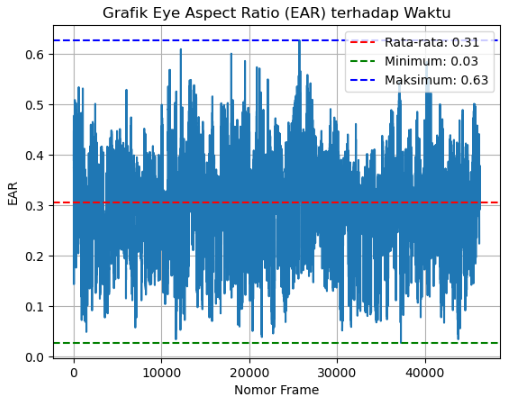
\includegraphics[width=0.75\linewidth]{figures/bab4/nilai ear.png}
             \caption{Grafik Nilai EAR}
             \label{Grafik Nilai EAR}
         \end{figure}

            Berdasarkan grafik pada Gambar \ref{Grafik Nilai EAR}, nilai EAR \textit{(Eye Aspect Ratio)} menunjukkan pola mengantuk berada dibawah rata-rata. Hal ini sesuai dengan teori yang menyatakan bahwa semakin kecil nilai EAR menunjukkan bahwa kondisi mata semakin tertutup. Namun perlu ditentukan ambang batas \textit{threshold} dimana nilai EAR menunjukkan mengantuk dengan kesalahan terkecil.
            
            Pada penentuan ambang batas tersebut akan dicoba ekstrak video dengan rentang nilai di bawah rata-rata yaitu $0.18 - 0.30$ dan diatas rata-rata yaitu $0.32 - 0.40$. Pemilihan rentang tersebut berdasarkan pola hasil visualisai nilai EAR yang menunjukkan pada rentang tersebut terdapat pola mata mengantuk. Selanjutnya akan di ekstrak video menjadi gambar kedalam dua kelas yaitu kantuk dan tidak kantuk. Tujuan mencoba bebera nilai ini untuk melihat di angka berapa nilai EAR dapat menentukan kantuk dan tidak kantuk dengan nilai kesalahan terkecil menggunakan Persamaan \ref{rumus error}. Nilai EAR yang dicoba untuk melakukan ekstraksi video menjadi gambar dapat di lihat pada Tabel \ref{Penentuan Nilai EAR} berikut.\\


            \begin{table}[h]
            \centering
            \caption{Eksperimen Penentuan Nilai EAR}
            \begin{tabular}{ccccc}
                \toprule
                 \textbf{No} &\textbf{Nilai EAR} & \textbf{Jumlah Kantuk} & \textbf{Salah Deteksi} & \textbf{\textit{Error (\%)}} \\
                \midrule
                   
                      
                         1 & 0.40 & 1863 & 1715 & 92.05 \\
                         2 &  0.38 & 1613 & 1465 & 90.82 \\
                         3 & 0.36 & 1332 & 1184 & 88.88 \\
                         4 &  0.34 & 1069 & 921  & 86.15 \\
                         5 &  0.32 & 796  & 648  & 81.00 \\
                         6 & \textbf{0.30} &\textbf{ 570} & \textbf{320} & \textbf{56.14} \\
                         7 & 0.28 & 400 & 220 & 55.00 \\
                         8 &  0.26 & 274 & 124 & 45.25 \\
                         9 &  0.24 & 196 & 104 & 53.06 \\
                         10 &  0.22 & 133 & 60& 45.11 \\
                         11 &  0.20 & 101 & 36  & 35.64 \\
                         12 &  0.18 & 87  & 30  & 34.48\\
    
                    \bottomrule
                \end{tabular}
                \label{Penentuan Nilai EAR}
            \end{table}

           Ekstraksi video dilakukan dengan cara membagi hasil setiap gambar menjadi dua kategori, yaitu kantuk dan tidak kantuk. Selanjutnya, dilakukan pemeriksaan kembali terhadap hasil ekstrak pada kategori kantuk untuk mengetahui jumlah sampel yang salah diklasifikasikan sebagai mengantuk, pada sesungguhnya tidak mengantuk. Hal ini dilakukan secara empiris atau melihat langsung hasil ekstraksi.


            Pada tabel \ref{Penentuan Nilai EAR} ditemukan bahwa nilai EAR yang berada di atas rata-rata memiliki nilai \textit{error} yang tinggi yaitu diatas angka $ 81\%$, hal ini menunjukkan bahwa nilai EAR diatas rata-rata tidak dapat mengelompokkan data dengan baik. Nilai \textit{error} di bawah rata-rata menunjukkan angkanya mengecil, hal ini menunjukkan semakin sedikitnya terjadi kesalahan prediksi. Visualisasi nilai EAR ditampilkan pada Gambar \ref{Eksperimen Penentuan Nilai EAR} berikut.

             \begin{figure}[H]
             \centering
                 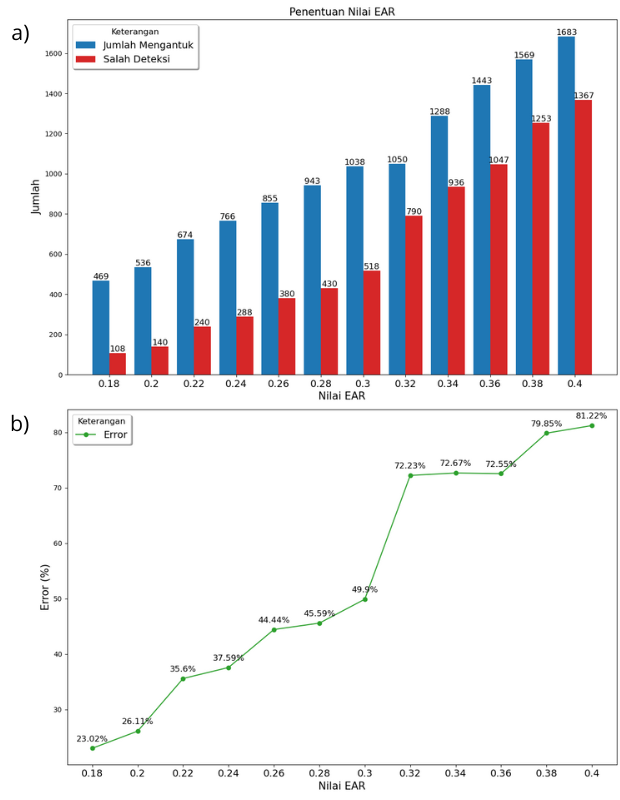
\includegraphics[width=0.8\textwidth]{figures/bab4/penentuan nilai ear.png}
                 \caption{a) Percobaan Nilai EAR, b) Nilai \textit{Error} EAR}
                 \label{Eksperimen Penentuan Nilai EAR}
             \end{figure}


          Dari hasil visualisasi pada Gambar \ref{Eksperimen Penentuan Nilai EAR} menunjukkan pola bahwa semakin besar nilai EAR jumlah yang terdeteksi kantuk juga semakin besar, namun nilai \textit{error }juga sangat kecil. Pola ini sesuai dengan teori yang menyatakan semakin kecil nilai EAR menunjukkan bahwa kondisi mata sedang tertutup atau mengantuk. Sehingga pada penentuan nilai EAR penelitian ini akan digunakan dengan nilai kesalahan atau \textit{error} yang terkecil yaitu dengan EAR sebesar 0.18 dengan \textit{error} sebesar $34.48\%$\\

    

\subsubsection{\textit{Mouth Aspect Ratio} (MAR)}
    
    
             \begin{figure}[H]
                 \centering
                 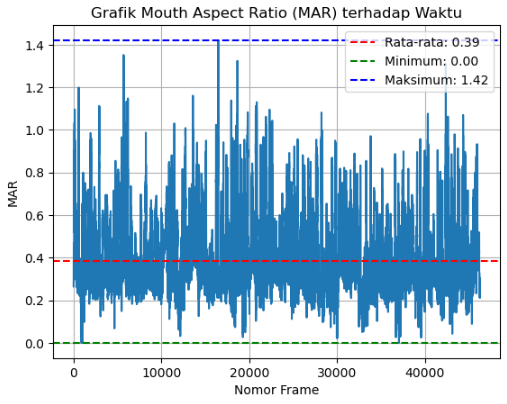
\includegraphics[width=0.8\linewidth]{figures/bab4/nilai mar.png}
                 \caption{Grafik Nilai MAR}
                 \label{Grafik Nilai MAR}
             \end{figure}



        
            Berdasarkan grafik pada Gambar \ref{Grafik Nilai MAR}, nilai MAR \textit{(Mouth Aspect Ratio)} menunjukkan pola menguap berada atas rata-rata. Hal ini sesuai dengan teori yang menyatakan bahwa semakin besar nilai MAR menunjukkan bahwa kondisi mulut semakin terbuka lebar. Namun perlu ditentukan ambang batas dimana nilai MAR menunjukkan keadaan menguap dengan kesalahan terkecil. Pada visualisasi menunjukkan bahwa berada pada rentang $0.00 - 1.42$ dengan minimum $0.00$ hingga maksimum $1.42$, dan rata-rata sebesar $0.39$. 
            
            Pada penentuan ambang batas akan dicoba ekstrak video dengan rentang nilai di bawah rata-rata yaitu $0.40 - 0.30$ dan diatas rata-rata yaitu $0.42 - 0.52$. Pemilihan rentang tersebut berdasarkan pola hasil visualisai nilai MAR yang menunjukkan pada rentang tersebut terdapat mulut terbuka dengan lebar. Selanjutnya akan di ekstrak video menjadi gambar kedalam dua kelas yaitu menguap dan tidak menguap. Tujuan mencoba bebera nilai ini untuk 
            melihat dan menentukan di angka berapa nilai MAR dapat mengklasifikasikan setiap gambar menguap dan tidak menguap dengan nilai kesalahan terkecil menggunakan Persamaan \ref{rumus error}. Cara ini serupa dilakukan seperti penentuan nilai EAR sebelumnya.
            
            Nilai MAR dan hasil percobaan untuk melakukan ekstraksi video menjadi gambar dapat di lihat pada Tabel \ref{Penentuan Nilai MAR} berikut.\\


        
            \begin{table}[h]
            \centering
            \caption{a) Percobaan Nilai MAR, b) Nilai \textit{Error} MAR}
            \begin{tabular}{ccccc}
                \toprule
                \textbf{No} &\textbf{Nilai MAR} & \textbf{Jumlah Menguap} & \textbf{Salah Deteksi} & \textbf{\textit{Error} (\%)} \\
                \midrule
                          1 & 0.30 & 1683 & 1367 &  81.22 \\
                          2 & 0.32 & 1569 & 1253 & 79.85 \\
                          3 & 0.34 & 1443 & 1047 & 72.55 \\
                          4 & 0.36 & 1288 & 936  & 72.67 \\
                          5 & 0.38 & 1050 & 790  & 75.23\\
                         6 & \textbf{0.40} & \textbf{1038}& \textbf{518} &  \textbf{49.90} \\
                          7 & 0.42 & 943 & 430 & 45.59 \\
                          8 & 0.44 & 855 & 380 & 44.44 \\
                          9 & 0.46 & 766 & 288 & 37.59 \\
                          10 & 0.48 & 674 & 240 & 35.60 \\
                          11 & 0.50 & 536 & 140  & 26.11 \\
                          12 & 0.52 & 469 & 108 & 23.02 \\
                         
                    \bottomrule
                \end{tabular}
                \label{Penentuan Nilai MAR}
            \end{table}


         %Visualisasi nilai MAR yang diuju dapat dilihat pada Gambar \ref{Eksperimen Penentuan Nilai MAR} berikut.

         \begin{figure}[H]
               \centering
               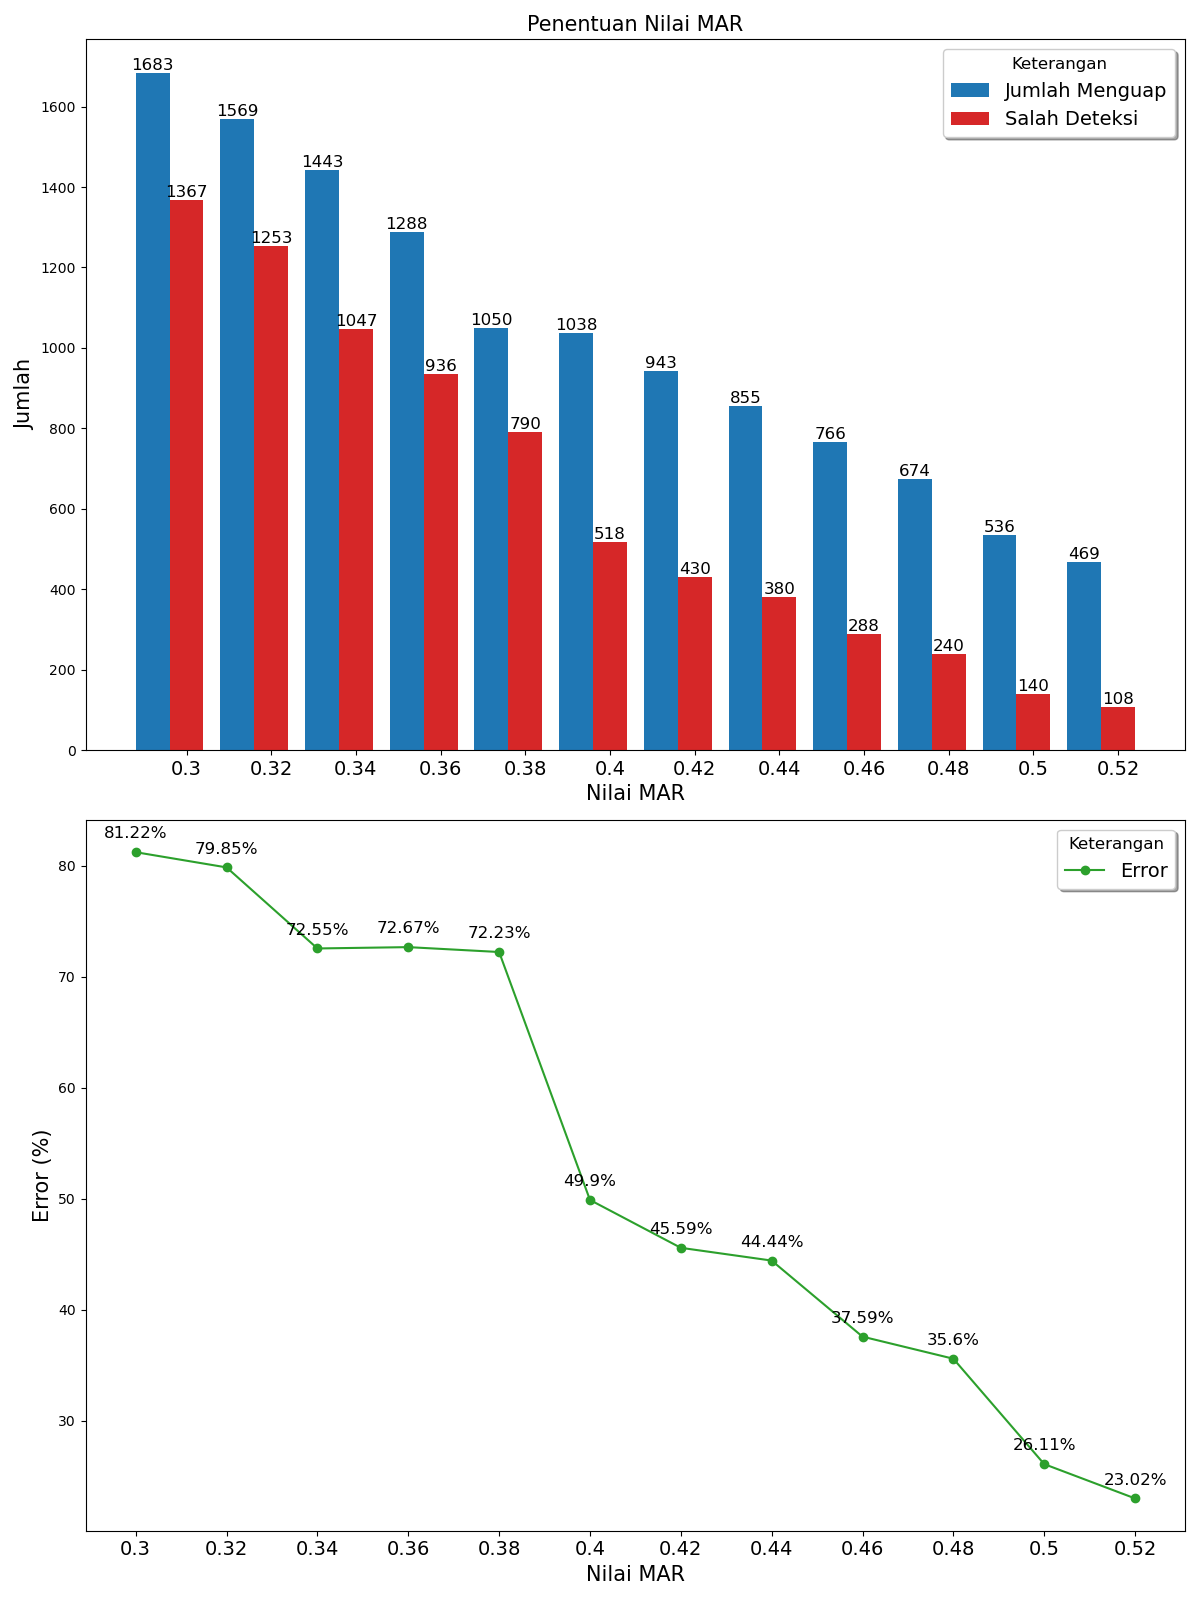
\includegraphics[width=0.8\textwidth]{figures/bab4/penentuan nilai mar.png}
               \caption{Eksperimen Penentuan Nilai MAR}
               \label{Eksperimen Penentuan Nilai MAR}

         \end{figure}

        Dari hasil visualisasi pada Gambar \ref{Eksperimen Penentuan Nilai MAR} menunjukkan pola bahwa semakin besar nilai MAR jumlah yang tereteksi 
        menguap juga semakin besar. Pola ini sesuai dengan teori yang menyatakan 
        semakin kecil nilai EAR menunjukkan bahwa kondisi mulut sedang terbuka lebar atau menguap. Sehingga pada penentuan nilai MAR penelitian ini akan digunakan dengan nilai kesalahan atau \textit{error} yang terkecil yaitu dengan MAR sebesar 0.52 dengan \textit{error} sebesar $23.02\%$\\



    Setelah dilakukan percobaan menggunakan beberapa nilai EAR (\textit{Eye Aspect Ratio}) dan MAR (\textit{Mouth Aspect Ratio}). Diperoleh nilai kesalahan terkecil untuk EAR sebesar 0.18 dan MAR 0.52. Kedua nilai ini digunakan untuk melakukan ekstraksi data secara keseluruhan.
    
\subsection{Ekstraksi Data}

     Setelah diperoleh nilai \textit{Eye Aspect Ratio }(EAR) dan \textit{Mouth Aspect Ratio} (MAR) 
     terbaik dengan nilai \textit{error} terkecil. Selanjutnya dilakukan ektraksi data secara keseluruhan 
     dari bentuk bentuk video (.avi) ke format gambar (.jpg). Data di ekstrak menjadi tiga kelas 
     yaitu "mengantuk \& menguap", "mengantuk \& tidak menguap", "menguap \& tidak mengantuk". 
     Proses ekstrak video agar menghasilkan data dengan format gambar sesuai dengan kelas yang 
     ditentukan dilakukan dengan kondisi seperti Gambar \ref{kondisi ear dan mar} berikut.


              \begin{figure}[H]
              \caption{Kondisi Penentuan Nilai EAR dan MAR}
               \centering
               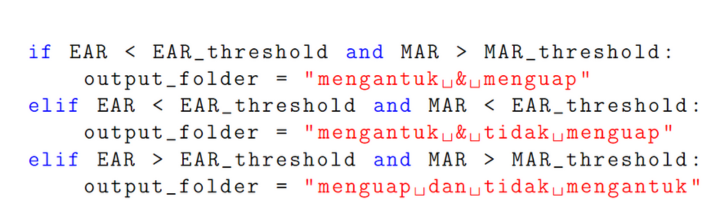
\includegraphics[width=0.90\textwidth]{figures/bab4/threshold.png}
               \caption{Pembagian Data}
               \label{kondisi ear dan mar}

         \end{figure}

     
   
    
    
    Setiap foto hasil ektraksi akan langsung otomatis masuk kedalam folder sesuai dengan kelas yang telah ditentukan. Pada ektraksi nilai \textit{thereshold} untuk EAR sebesar 0.18 dan nilai \textit{thereshold} MAR sebesar 0.58 kedua nilai ini diperoleh dari nilai terbaik hasil percobaan sebelumnya.

    \begin{enumerate}
        \item    Jika nilai EAR pada \textit{frame} tersebut lebih kecil dari EAR \textit{threshold} dan MAR lebih besar MAR \textit{threshold} foto akan masuk dalam folder "mengantuk \& menguap".

        \item Jika nilai EAR pada \textit{frame} tersebut lebih kecil dari EAR \textit{threshold} dan MAR lebih kecil
    dari MAR \textit{threshold} foto akan masuk dalam folder "mengantuk \& tidak menguap "


     \item  Jika nilai EAR pada \textit{frame} tersebut lebih besar dari EAR \textit{threshold} dan MAR lebih besar
    dari MAR \textit{threshold} foto akan masuk dalam folder "menguap \& tidak mengantuk"

    
        

    \end{enumerate}
    

     
     Hasil ekstrak data video menjadi gambar ditampilkan pada tabel \ref{Hasil Ekstraksi Data} berikut. 

       \begin{table}[H]
            \centering
            \caption{Hasil Ekstraksi Data}
            \begin{tabular}{cc}
                \toprule
                \textbf{Kelas} & \textbf{Hasil Ekstrak} \\
                \midrule  
                           Mengantuk dan Menguap & 1038  \\
                          Mengantuk tidak Menguap & 1304 \\
                           Menguap tidak Mengantuk& 2042  \\
                
                    \bottomrule
                \end{tabular}
                \label{Hasil Ekstraksi Data}
            \end{table}

        Pada tabel \ref{Hasil Ekstraksi Data} Ditemukan jumlah hasil ekstraksi untuk kelas "mengantuk dan menguap" 
        berjumlah 1038 gambar, "mengantuk dan tidak menguap" berjumlah 1304 gambar dan kelas yang terakhir
         "menguap tidak mengantuk" berjumlah 2042 gambar. Kondisi ini menunjukkan bahwa hasil ekstraksi 
         data pada setiap kelasnya \textit{imbalance}, hal ini dapat mempengaruhi hasil akurasi saat 
         dilakukan klasifikasi dengan CNN. Selanjutnya, untuk memperkaya jumlah data dan mengatasi 
         data \textit{imbalance} atau tidak seimbang pada setiap kelasnya dilakukan teknik augmentasi data. 
         Augmentasi data yang diterapkan adalah seperti \textit{zoom}, \textit{grayscal}e dan \textit{shear} 
         dengan metode \textit{oversampling} dengan konfigurasi seperti Tabel \ref{Perlakuan Augmentasi Data} berikut.

        
\begin{table}[H]
    \centering
    \caption{Perlakuan Augmentasi Data}
    \label{Perlakuan Augmentasi Data}
    \begin{tabular}{
        >{\raggedright\arraybackslash}p{1.0cm} 
        >{\raggedright\arraybackslash}p{2.5cm} 
        >{\raggedright\arraybackslash}p{9.3cm}}
        \hline
        \textbf{No} & \textbf{Augmentasi} & \textbf{Tujuan} \\
        \hline
        1 & \textit{zoom} & Memperbesar ukuran gambar dengan skala tertentu, nilai skala \textit{zoom} yang digunakan sebesar 0.3 atau 30\% dari gambar asli \\
        2 & \textit{sheer} & Melakukan transformasi yang memiringkan gambar ke arah tertentu, nilai \textit{shear} yang digunakan sebesar 90 derajat \\
        3 & \textit{grayscle} & Mengubah  gambar menjadi warna abu-abu atau hitam putih \\
        
        \hline
    \end{tabular}
\end{table}

     
        
        Hal ini bertujuan untuk membuat distribusi kelas menjadi seimbang. Augmentasi dilakukan dengan melakukan satu perlakukan untuk satu data pada jumlah kelas tertinggi. Kemudian jumlah ini menjadi acuan untuk kelas lainnya dengan maksimal data yang di augmentasi sebanyak jumlah data pada jumlah data kelas tertinggi. Sehingga pada masukan model CNN data menjadi seimbang. Jumlah data sebelum dan sesudah dilakukan augmentasi ditampilkan pada Tabel \ref{Hasil Augmentasi Data} berikut.
    


            \begin{table}[H]
            \centering
            \caption{Hasil Ekstraksi Data}
            \begin{tabular}{ccc}
                \toprule
                \textbf{Kelas} & \textbf{Hasil Ekstrak} & \textbf{Augmentasi }\\
                \midrule
                      
                           Mengantuk dan Menguap & 1038 & 4084 \\
                          Mengantuk tidak Menguap & 1304 & 4084 \\
                           Menguap tidak mengantuk& 2042 & 4084 \\
                
                    \bottomrule
                \end{tabular}
                \label{Hasil Augmentasi Data}
            \end{table}




    
    \subsection{Pembagian Data}
    
    Sebelum data dilatih, dilakukan pembagian data menjadi data 
    \textit{train} dan data \textit{test}. Pembagian data ini 
    dilakukan dengan menggunakan metode \textit{KFold Cross Validation}. 
    Teknik ini melibatkan pembagian data menjadi beberapa \textit{subset}. 
    Menerapkan pembagian data dengan \textit{KFold Cross Validation} 
    bertujuan untuk mencegah \textit{overfitting}, 
    menghasilkan estimasi performa model yang stabil, 
    membandingkan model, dan memperkirakan generalisasi model. 
    Dengan hal ini dapat memperoleh perkiraan kinerja model yang 
    lebih akurat dan membantu dalam pemilihan model terbaik pada 
    saat \textit{training} dilakukan. 
    
    Peneliti menerapkan \textit{fold} sebesar lima untuk mempekecil waktu komputasi. Sehingga keseluruhan data dibagi menjadi lima lipatan dan dilatih sebanyak lima kali berdasarkan jumlah \textit{fold }yang telah ditentukan sebelumnya. Pembagian data diilustrasikan seperti pada Gambar \ref{Pembagian Data} berikut.

         \begin{figure}[H]
               \centering
               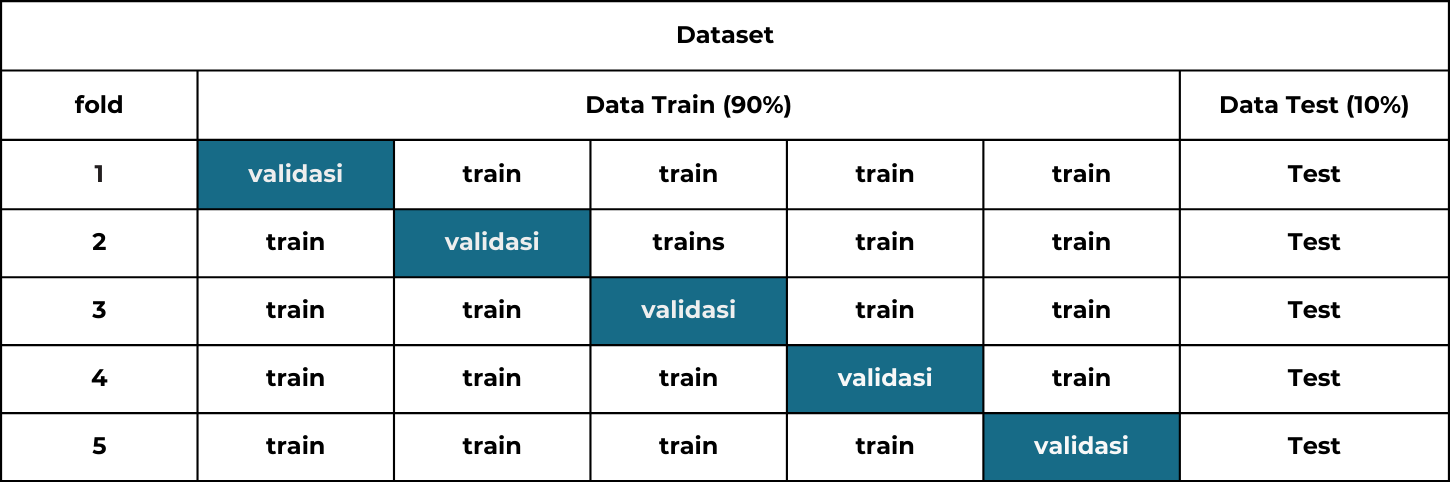
\includegraphics[width=0.90\textwidth]{figures/bab4/kfold.png}
               \caption{Pembagian Data}
               \label{Pembagian Data}

         \end{figure}



    Dari keseluruhan data hasil ekstraksi dan augmentasi diperoleh jumlah data sebanyak 12.252 gambar, 10\% dari keselurahan data dibagi menjadi data \textit{test} yaitu sebanyak 1227 gambar. Pada data \textit{test} jumlah data untuk setiap kelasnya sama yaitu sebanyak 409 gambar. Untuk data 90\% dibagi berdasarkan jumlah \textit{KFold} yang telah ditetapkan yaitu $k = 5$, sehingga diperoleh untuk setiap \textit{foldnya} berjumlah sebanyak 2205 gambar dengan jumlah data setiap data kelasnya seimbang.
    



\section{Arsitektur CNN}

    Arsitektur CNN yang digunakan memiliki \textit{input shape} sebesar $ 64 x 64 $ piksel dan terdapat beberapa \textit{layer} yang digunakan dalam pembuatan model untuk melakukan klasifikasi. Berikut adalah ringkasan arsitektur yang digunakan:

    \begin{enumerate}
        \item     \textit{Convolutional Layers}: Terdapat tiga blok \textit{convolutional layer} yang masing-masing terdiri dari dua \textit{layer} Conv2D dengan aktivasi ReLU dan \textit{padding} yang sama. Blok pertama memiliki 32 filter, blok kedua memiliki 64 filter, dan blok ketiga memiliki 128 filter.
    
        \item  \textit{Batch Normalization}: Dilakukan setelah setiap blok \textit{convolutional }untuk mempercepat proses konvergensi dan mengurangi \textit{overfitting}.
    
        \item \textit{Max Pooling Layers}: Setelah setiap blok \textit{convolutional}, dilakukan \textit{max pooling} dengan ukuran sebesar (2,2) untuk mengurangi dimensi gambar.
    
       \item  \textit{Dropout}: Setelah \textit{max pooling} terakhir, dilakukan \textit{dropout} dengan nilai 0.2 untuk mengurangi \textit{overfitting}.
    
        \item \textit{Flatten Layer}: Digunakan untuk mengubah \textit{output} dari \textit{layer} sebelumnya menjadi vektor satu dimensi.
    
        \item \textit{Dense Layers:} Terdapat dua \textit{layer dense} setelah \textit{flatten layer}. \textit{Layer} pertama memiliki 256 unit dengan aktivasi ReLU dan \textit{layer} terakhir memiliki tiga unit dengan aktivasi \textit{softmax}, sesuai dengan jumlah kelas yang ada.

    \end{enumerate}

    Untuk desain arsitektur \textit{Convolutional Neural Network} (CNN) yang digunakan ditampilkan pada Tabel 
    \ref{Desain arsitektur} berikut.

    

    \begin{table}[H]
        \centering
        \scriptsize
        \caption{Desain Arsitektur}
        \label{Desain arsitektur}
        \renewcommand{\arraystretch}{1.5}
        \begin{tabular}{p{1cm}p{4.5cm}p{4cm}p{2.5cm}}
        \hline
        \textbf{No} & \textbf{Layer (type)}   & \textbf{Output Shape} & \textbf{Parameters}  \\ \hline
        
        1 & conv2d                   & (64, 64, 32)   & 896     \\ 
        2 & conv2d\_1                & (64, 64, 32)   & 9248    \\ 
        3 & batch\_normalization     & (64, 64, 32)   & 128     \\ 
        4 & max\_pooling2d           & (32, 32, 32)   & 0       \\ 
        5 & conv2d\_2                & (32, 32, 64)   & 18496   \\ 
        6 & conv2d\_3                & (32, 32, 64)   & 36928   \\ 
        7 & batch\_normalization\_1  & (32, 32, 64)   & 256     \\ 
        8 & max\_pooling2d\_1        & (16, 16, 64)   & 0       \\ 
        9 & conv2d\_4                & (16, 16, 128)  & 73856   \\ 
        10 & conv2d\_5                & (16, 16, 128)  & 147584  \\ 
        11 & batch\_normalization\_2  & (16, 16, 128)  & 512     \\ 
        12 & max\_pooling2d\_2        & (8, 8, 128)    & 0       \\ 
        13 & dropout                  & (8, 8, 128)    & 0       \\ 
        14 & flatten                  & (8192)         & 0       \\ 
        15 & dense                    & (256)          & 2097408 \\ 
        16 & dense\_1                 & (3)            & 771     \\ \hline
        \end{tabular}
    \end{table}





\section{Pengujian Model CNN}

    Dalam rangka menguji model, beberapa skenario dijalankan untuk mengidentifikasi model terbaik.
     Penelitian ini menguji beberapa parameter, sebagaimana dijelaskan pada Tabel \ref{Pengujian Parameter}, dengan 
     tujuan untuk menentukan parameter optimal.  Akurasi \textit{test} yang dimaksud pada pengujian 
     ini adalah menggunakan data validasi, sedangkan \textit{activation function} yang digunakan 
     hanya pada \textit{hidden layer}.


    
        
\subsection{Pengujian \textit{Learning Rate} dan \textit{Activation Layer}}

    Pada pengujian ini menampilkan evaluasi dari \textit{accuracy} \textit{train}, \textit{validation}, \textit{test}, \textit{precision}, \textit{recall} dan \textit{F1-Score}.

\subsubsection{\textit{Learning Rate} 0.01}

        \begin{table}[H]
        \centering
        \caption{Pengujian \textit{Learning Rate} 0.01 }
        \begin{tabular}{ccccc}
            \toprule
            \multicolumn{5}{c}{\textit{Learning Rate} 0.01} \\ \hline
            
            \textbf{\textit{Activation}} & \multicolumn{1}{c}{\textbf{\textit{KFold}}} & \textbf{\textit{Train Acc (\%)} } & \textbf{\textit{Val Acc (\%)}} & \textbf{\textit{Test Acc (\%)}}  \\
    
            \midrule
            \multirow{5}{*}{ReLU} 
            & 1 & 48.19 & 48.48 & 54.42  \\
            & 2 & 67.88 & 62.13 & 63.08 \\
            & 3 & 51.34 & 46.77 & 51.81 \\
            & 4 & 32.68 & 33.93 & 35.29 \\
            & 5 & 36.14 & 33.39 & 45.91 \\ 
            & \textbf{\textit{mean}}& \textbf{47.24 }& \textbf{44.94} & \textbf{50.10} \\ \hline

    
            \multirow{5}{*}{Sigmoid}
            & 1 & 33.46 & 33.56 & 33.83  \\
            & 2 & 33.97 & 34.14 & 34.14 \\
            & 3 & 33.12 & 32.57 & 34.34 \\
            & 4 & 34.24 & 32.84 & 34.16 \\
            & 5 & 34.03 & 33.12 & 33.75 \\
            & \textit{\textbf{mean}}& \textbf{33.76} & \textbf{33.24} &\textbf{34.04} \\ 
                        \hline
    
            \multirow{5}{*}{Softmax}
            & 1 & 33.10 & 32.47 & 33.92 \\
            & 2 & 33.63 & 32.97 & 33.51 \\
            & 3 & 33.10 & 33.12 & 34.21  \\
            & 4 & 33.27 & 32.66 & 33.71 \\
            & 5 & 33.38 & 32.94 & 33.80 \\
            & \textit{\textbf{mean}}& \textbf{33.29} & \textbf{32.83} &\textbf{33.83} \\ 
    

            \bottomrule
            \end{tabular}
            \label{Pengujian Learning Rate 0.01 }
        \end{table}

    Pengujian fungsi \textit{activation function} dengan \textit{learning rate} 0.01 
    pada ReLU diperoleh rata-rata akurasi untuk \textit{training} sebesar 47.24\%, validasi sebesar 44.94\% dan test sebesar 50.10\%. Namun akurasi model cukup bervariasi di setiap iterasi \textit{KFold}, dapat dilihat pada akurasi \textit{training} diperoleh nilai terkecil sebesar 32.68\% dan terbesar 67.88\%.
    Hal ini menunjukkan bahwa model sensitif terhadap pembagian data. Pada \textit{activation function} \textit{sigmoid} diperoleh rata-rata akurasi untuk \textit{training} sebesar 33.76\%, validasi sebesar 33.24\% dan test sebesar 34.04\%. Akurasi pada \textit{sigmoid} stabil di setiap iterasi \textit{KFold} tapi akurasi yang dihasilkan jauh lebih kecil jika dibandingkan dengan ReLU.
    
    Pada \textit{activation function} \textit{softmax} akurasi rata-rata untuk \textit{training} sebesar 33.29\%, validasi sebesar 33.83\% dan test sebesar 33.83\%. Akurasi pada \textit{softmax} juga stabil di setiap iterasi \textit{KFold} tapi akurasi yang dihasilkan lebih kecil jika dibandingkan dengan ReLU dan \textit{sigmoid}. Pada pengujian \textit{activation function} untuk \textit{learning rate} 0.01 \textit{activation function} terbaik adalah ReLU dengan rata-rata akurasi untuk \textit{training} sebesar 47.24\%, validasi sebesar 44.94\% dan test sebesar 50.10\%.

    

        \begin{table}[H]
        \centering
        \caption{Evaluasi \textit{Learning Rate} 0.01}
        \begin{tabular}{ccccc}
            \toprule
            \multicolumn{5}{c}{\textit{Learning Rate} 0.01} \\ \hline
            
            \textbf{\textit{Activation}} & \multicolumn{1}{c}{\textbf{\textit{KFold}}} & \textbf{\textit{Precision (\%)} } & \textbf{\textit{Recall (\%)}} & \textbf{\textit{F1-Score (\%)}}  \\
    
            \midrule
            \multirow{5}{*}{ReLU} 

            & 1 & 81.54 & 54.42 & 63.25  \\
            & 2 & 76.90 & 63.08 & 65.95 \\
            & 3 & 82.63 & 51.81 & 62.80\\
            & 4 & 91.16 & 35.29 & 48.00\\
            & 5 & 80.00 & 45.91 & 54.39 \\ 
            & \textbf{\textit{mean}}& \textbf{82.44} & \textbf{50.10} & \textbf{58.87} \\ \hline
            
            \multirow{5}{*}{Sigmoid}
            & 1 &  33.33 & 33.83 & 50.55  \\
            & 2 &  33.33  & 34.14 & 50.59 \\
            & 3 &  33.33  & 34.34 & 51.13 \\
            & 4 &  33.33  & 34.16 & 50.92 \\
            & 5 &  33.33  & 33.75 & 50.47 \\
            & \textit{\textbf{mean}}& \textbf{33.33} & \textbf{34.04} &\textbf{50.73} \\ 
                        \hline
    
            \multirow{5}{*}{Softmax}
            & 1 & 33.33  & 33.92 & 50.66 \\
            & 2 & 33.33  & 33.51 & 50.20 \\
            & 3 & 33.33  & 34.21 & 50.98  \\
            & 4 & 33.33  & 33.71 & 50.42 \\
            & 5 & 33.33  & 33.80 & 50.52 \\
            & \textit{\textbf{mean}}& \textbf{33.33} & \textbf{33.83} &\textbf{50.55} \\ 
    

            \bottomrule
        \end{tabular}
        \label{Evaluasi Learning Rate 0.01 }
    \end{table}

      Evaluasi model pada \textit{activation function} dengan \textit{learning rate} 0.01 menunjukkan bahwa \textit{activation function} \textit{ReLU} menghasilkan nilai rata-rata \textit{precision} sebesar 82,44\%, \textit{recall} 50,10\%, dan\textit{ F1-Score} 58,87\%. Hal ini menunjukkan kecenderungan \textit{activation function} \textit{ReLU} untuk memprioritaskan prediksi positif daripada mengidentifikasi semua contoh positif. Hal ini terlihat dari nilai \textit{precision} yang jauh lebih tinggi dibandingkan \textit{recall}.

     Pada \textit{activation function} \textit{sigmoid} diperoleh nilai rata-rata pada \textit{precision} sebesar 33.33\%, \textit{recall} sebsar 34.04\% dan\textit{ F1-Score} sebesar 50.73\%. Hasil untuk \textit{sigmoid} menunjukkan bahwa model hanya dapat memprediksi satu kelas saja, hal ini dapat di lihat pada nilai \textit{precision} yang sama setiap iterasi KFold. Pada \textit{activation function} \textit{softmax} diperoleh nilai rata-rata pada \textit{precision} sebesar 33.33\%, \textit{recall} sebesar 33.83\% dan \textit{F1-Score} sebesar 50.55\%.
     Berdasarkan hasil evaluasi, \textit{activation function} ReLU menghasilkan performa terbaik dengan 
     rata-rata \textit{F1-Score} tertinggi. \textit{Sigmoid} dan \textit{softmax} memiliki performa yang jauh lebih rendah dan perlu dioptimalkan lebih lanjut.


 

    \subsubsection{\textit{Learning Rate} 0.001}
    
    \begin{table}[H]
        \centering
        \caption{Pengujian \textit{Learning Rate} 0.001 }
        \begin{tabular}{ccccc}
            \toprule
            \multicolumn{5}{c}{\textit{Learning Rate} 0.001} \\ \hline
            
            \textbf{\textit{Activation}} & \multicolumn{1}{c}{\textbf{\textit{KFold}}} & \textbf{\textit{Train Acc (\%)} } & \textbf{\textit{Val Acc (\%)}} & \textbf{\textit{Test Acc (\%)}}  \\
    
            \midrule
            \multirow{5}{*}{ReLU} 
            & 1 & 91.41 & 86.98 & 90.70  \\
            & 2 & 90.84 & 86.12 & 91.84 \\
            & 3 & 89.42 & 80.49 & 87.70 \\
            & 4 & 91.10 & 90.79 & 92.24 \\
            & 5 & 91.99 & 90.42 & 91.74  \\
            & \textit{\textbf{mean}}& \textbf{90.95} & \textbf{86.96} &\textbf{ 90.84} \\ \hline
    
            \multirow{5}{*}{Sigmoid}
            & 1 &  93.72 & 65.17 & 87.30  \\
            & 2 &  91.15 & 47.21 & 69.52 \\
            & 3 &  89.24 & 60.93 & 86.25 \\
            & 4 &  33.56 & 32.98 & 34.16 \\
            & 5 &  59.35 & 40.01 & 46.23 \\
            & \textit{\textbf{mean}}& \textbf{73.40} & \textbf{49.26} &\textbf{64.69} \\ 
                        \hline
    
            \multirow{5}{*}{Softmax}
            & 1 & 32.99 & 31.79 & 34.28 \\
            & 2 & 33.27 & 33.65 & 33.65 \\
            & 3 & 33.04 & 32.35 & 34.93  \\
            & 4 & 33.18 & 32.57 & 33.93 \\
            & 5 & 33.20 & 32.94 & 32.94 \\
            & \textit{\textbf{mean}}& \textbf{33.13} & \textbf{32.66} &\textbf{33.94} \\ 

            \bottomrule
        \end{tabular}
        \label{Pengujian Learning Rate 0.001}
    \end{table}

    Pengujian \textit{activation function} untuk \textit{learning rate} 0.001 
    pada \textit{ReLU} diperoleh rata-rata akurasi untuk \textit{training} sebesar 91.41\%, validasi sebesar 86.96\% dan test sebesar 90.84\%. Pada \textit{learning rate} 0.001 terjadi peningkatan akurasi yang signifikan dari akurasi menggunakan \textit{learning rate} 0.01. Sebelumnya hanya diperoleh rata-rata akurasi untuk \textit{training} sebesar 47.24\%, validasi sebesar 44.94\% dan test sebesar 50.10\%. Pada \textit{learning rate} 0.001 juga diperoleh akurasi setiap iterasi \textit{KFold} jauh lebih stabil dibandingkan sebelumnya. 

    \textit{Activation function} \textit{sigmoid} memiliki akurasi rata-rata untuk \textit{training} sebesar 73.40\%, validasi sebesar 49.26\% dan test sebesar 64.69\%. Penggunaan \textit{learning rate} 0.001 untuk \textit{activation function} \textit{sigmoid} juga mengalami peningkatan yang tinggi dari sebelumnya rata-rata akurasi untuk \textit{training} sebesar 33.33\%, validasi sebesar 34.04\% dan test sebesar 50.73\%. Namun pada setiap iterasi \textit{KFold} akurasi sangat tidak stabil hal ini dibuktikan terdapat akurasi tertinggi sebesar 93.72\% dan terendah sebesar 33.56\%. Hal ini menunjukkan pembagian data sangat sensitif pada \textit{activation function} sigmoid. Pada \textit{activation function} \textit{softmax} memiliki akurasi rata-rata untuk \textit{training} sebesar 33.13\%, validasi sebesar 32.66\% dan test sebesar 33.94\%. Pada \textit{softmax} tidak ada perubahan yang cukup signifikan dari penggunaan \textit{learning rate} sebelumnya. 

     Penurunan \textit{learning rate} dari 0.01 ke 0.001 menunjukkan pengaruh yang signifikan terhadap kinerja \textit{activation function} \textit{ReLU} dan \textit{sigmoid}. Namun pada perubahan \textit{learning rate} tidak menunjukkan efek yang substansial pada \textit{activation function} \textit{softmax}.
    
    
    
    

   

    \begin{table}[H]
        \centering
        \caption{Evaluasi \textit{Learning Rate} 0.001 }
        \begin{tabular}{ccccc}
            \toprule
            \multicolumn{5}{c}{\textit{Learning Rate} 0.001} \\ \hline
            
            \textbf{\textit{Activation}} & \multicolumn{1}{c}{\textbf{\textit{KFold}}} & \textbf{\textit{Precision (\%)} } & \textbf{\textit{Recall (\%)}} & \textbf{\textit{F1-Score (\%)}}  \\
    
            \midrule
            \multirow{5}{*}{ReLU} 

            & 1 & 91.89 & 90.70 & 90.80  \\
            & 2 & 92.04 & 91.83 & 91.80 \\
            & 3 & 87.82 & 87.70 & 87.72\\
            & 4 & 92.20 & 92.24 & 92.21\\
            & 5 & 91.68 & 91.74 & 91.70 \\
            & \textit{\textbf{mean }} & \textbf{91.12} & \textbf{90.84} & \textbf{90.84 }\\ \hline

            
            \multirow{5}{*}{Sigmoid}
            & 1 & 88.20 & 87.30 & 87.20  \\
            & 2 & 83.43 & 69.52 & 73.23 \\
            & 3 & 86.43 & 86.25 & 86.09 \\
            & 4 & 100.00 & 34.16 & 50.92 \\
            & 5 & 72.05 & 46.23 & 55.97 \\
            & \textit{\textbf{mean}}& \textbf{86.02} & \textbf{64.69} &\textbf{70.68} \\ 
                        \hline
    
            \multirow{5}{*}{Softmax}
            & 1 & 33.33  & 34.28 & 51.06 \\
            & 2 & 33.33  & 33.65 & 50.35 \\
            & 3 & 33.33  & 34.93 & 51.78  \\
            & 4 & 33.33  & 33.93 & 50.67 \\
            & 5 & 33.33  & 32.94 & 49.55 \\
            & \textit{\textbf{mean}}& \textbf{33.33} & \textbf{33.94} &\textbf{50.68} \\ 
    

            \bottomrule
        \end{tabular}
        \label{Evaluasi Learning Rate 0.001 }
    \end{table} 

\vspace{1cm}


    Evaluasi model untuk \textit{activation function} dengan \textit{learning rate} 0.001 menunjukkan bahwa \textit{activation function} \textit{ReLU} menghasilkan nilai rata-rata \textit{precision} sebesar 91.12\%, \textit{recall} 90.84\%, dan \textit{ F1-Score} 90.84\%. Hasil ini jauh lebih baik dari pada penggunaan \textit{learning rate} 0.01 karena nilai rata-rata yang lebih tinggi dan untuk setiap metriks yang dihasilkan juga stabil. 
    
     Pada \textit{activation function} \textit{sigmoid} diperoleh nilai rata-rata pada \textit{precision} sebesar 86.02\%, \textit{recall} sebsar 64.69\% dan\textit{ F1-Score} sebesar 70.68\%. Hasil pada \textit{sigmoid} menunjukkan perubahaan \textit{learning rate} menjadi 0.01 cukup berarti, hal ini dibuktikan adanya peningkatan nilai pada setiap mariks evaluasi. Sementara pada \textit{activation function} \textit{softmax} diperoleh nilai rata-rata pada \textit{precision} sebesar 33.33\%, \textit{recall} sebsar 33.94\% dan\textit{ F1-Score} sebesar 50.68\%.
     Perubahan \textit{learning rate} pada \textit{activation function} \textit{sigmoid} tidak memiliki hasil yang berarti. 
     
     Pada penggunaan \textit{learning rate} 0.001 hasil evaluasi menunjukkan \textit{activation function} terbaik diperoleh pada ReLU nilai \textit{ F1-Score} 90.84\%.
     
  

    

   \subsubsection{\textit{Learning Rate} 0.0001} 

   
        \begin{table}[H]
        \centering
        \caption{Pengujian \textit{Learning Rate} 0.0001 }
        \begin{tabular}{ccccc}
            \toprule
            \multicolumn{5}{c}{\textit{Learning Rate} 0.0001} \\ \hline
            
            \textbf{\textit{Activation}} & \multicolumn{1}{c}{\textbf{\textit{KFold}}} & \textbf{\textit{Train Acc (\%)} } & \textbf{\textit{Val Acc (\%)}} & \textbf{\textit{Test Acc (\%)}}  \\
    
            \midrule
            \multirow{5}{*}{ReLU} 

            & 1 & 90.46 & 87.02 & 91.88 \\
            & 2 & 93.00 & 89.02 & 91.97 \\
            & 3 & 97.25 & 83.03 & 90.29 \\
            & 4 & 90.22 & 89.11 & 90.69 \\
            & 5 & 93.02 & 92.00 & 93.69 \\ 
            & \textit{\textbf{mean}}& \textbf{92.79} & \textbf{88.03} &\textbf{91.70.} \\ 
            \hline


            \multirow{5}{*}{Sigmoid}
            & 1 &  84.93 & 69.75 & 76.73  \\
            & 2 &  71.23 & 41.40 & 69.43 \\
            & 3 &  68.32 & 35.34 & 63.15 \\
            & 4 &  71.27 & 57.89 & 70.37 \\
            & 5 &  65.51 & 37.47 & 46.09 \\
            & \textit{\textbf{mean}}& \textbf{72.25} & \textbf{48.37} &\textbf{65.15} \\ 
                        \hline
    
            \multirow{5}{*}{Softmax}
            & 1 & 33.71 & 31.79 & 31.79 \\
            & 2 & 33.01 & 33.24 & 33.24 \\
            & 3 & 33.01 & 32.71 & 32.71  \\
            & 4 & 32.92 & 33.48 & 33.48 \\
            & 5 & 33.43 & 32.94 & 32.94 \\
            & \textit{\textbf{mean}}& \textbf{33.21} & \textbf{32.83} &\textbf{32.83} \\ 

            \bottomrule
        \end{tabular}
        \label{Pengujian Learning Rate 0.0001 }
    \end{table}

    Pengujian \textit{activation function} untuk \textit{learning rate} 0.0001 
    pada \textit{ReLU} diperoleh rata-rata akurasi untuk \textit{training} sebesar 92.79\%, validasi sebesar 88.03\% dan test sebesar 91.70\%. Pada \textit{learning rate} 0.0001 terjadi peningkatan akurasi sekitar dua persen dari penggunaan \textit{learning rate} 0.001. 
    
    Penggunaan \textit{activation function} \textit{sigmoid} memiliki akurasi rata-rata untuk \textit{training} sebesar 72.25\%, validasi sebesar 48.37\% dan test sebesar 65.15\%. Penggunaan \textit{learning rate} 0.0001 untuk \textit{activation function} \textit{sigmoid} tidak terdapat pola peningkatan akurasi malah mengalami penurunan akurasi sekitar satu persen. Pada hasil ini menunjukkan bahwa penurunan nilai \textit{learning rate} pada \textit{activation function} \textit{sigmoid}
    tidak selalu mengalami peningkatan akurasi. 

    Pada \textit{activation function} \textit{softmax} memiliki akurasi rata-rata untuk \textit{training} sebesar
     33.21\%, validasi sebesar 32.83\% dan test sebesar 32.83\%. Hasil \textit{activation function} \textit{softmax} tidak mengalami perubahan yang begitu besar dari penggunaan \textit{learning rate} 0.0001, 0.001, 0.01, Sehingga dapat disimpulkan pengaruh \textit{learning rate} untuk \textit{softmax }tidak cukup berpengaruh.



    \begin{table}[H]
        \centering
        \caption{Evaluasi \textit{Learning Rate} 0.0001 }
        \begin{tabular}{ccccc}
            \toprule
            \multicolumn{5}{c}{\textit{Learning Rate} 0.0001} \\ \hline
            
            \textbf{\textit{Activation}} & \multicolumn{1}{c}{\textbf{\textit{KFold}}} & \textbf{\textit{Precision (\%)} } & \textbf{\textit{Recall (\%)}} & \textbf{\textit{F1-Score (\%)}}  \\
    
            \midrule
            \multirow{5}{*}{ReLU} 
            
            & 1 & 92.09 & 91.88 & 91.87 \\
            & 2 & 92.28 & 91.97 & 91.95 \\
            & 3 & 91.11 & 90.29 & 90.35 \\
            & 4 & 90.77 & 90.69 & 90.70 \\
            & 5 & 93.84 & 93.69 & 93.71 \\ 
            & \textit{\textbf{mean}}& \textbf{91.01} & \textbf{91.70} &\textbf{91.71} \\ 
            \hline


            
            \multirow{5}{*}{Sigmoid}
            & 1 &  82.05 & 76.73 & 77.49  \\
            & 2 &  70.47 & 69.43 & 69.65 \\
            & 3 &  71.52 & 63.15 & 65.22  \\
            & 4 &  70.94 & 70.37 & 70.51 \\
            & 5 &  72.78 & 46.09 & 51.60 \\
            & \textit{\textbf{mean}}& \textbf{73.55} & \textbf{65.15} &\textbf{66.89} \\ 
                        \hline
    
            \multirow{5}{*}{Softmax}
            & 1 & 33.33  & 31.79 & 48.24 \\
            & 2 & 33.33  & 33.24 & 49.89 \\
            & 3 & 33.33  & 32.71 & 49.29 \\
            & 4 & 33.33  & 33.48 & 50.16 \\
            & 5 & 33.33  & 32.94 & 49.55 \\
            & \textit{\textbf{mean}}& \textbf{33.33} & \textbf{32.83} &\textbf{49.42} \\ 
    

            \bottomrule
        \end{tabular}
        \label{Evaluasi Learning Rate 0.0001 }
    \end{table}

      Evaluasi model pada \textit{activation function} dengan \textit{learning rate} 0.0001 \textit{activation function} \textit{ReLU} menghasilkan nilai rata-rata \textit{precision} sebesar 91.01\%, \textit{recall} 91.70\%, dan\textit{ F1-Score} 91.71\%. Pada 
      Penggunaan \textit{learning rate} 0.0001 hasil prediksi setiap kelasnya cukup stabil di bandingkan sebelumnya. 
      
      Pada \textit{activation function} \textit{sigmoid} diperoleh nilai rata-rata pada \textit{precision} sebesar 73.55\%, \textit{recall} sebesar 65.15\% dan\textit{ F1-Score} sebesar 66.89\%. Hasil untuk \textit{sigmoid} menunjukkan lebih rendah dengan penggunaan \textit{learning rate} 0.001 yaitu dengan nilai rata-rata pada \textit{precision} sebesar 86.02\%, \textit{recall} sebsar 64.69\% dan\textit{ F1-Score} sebesar 70.68\%. Sementara pada \textit{activation function} \textit{softmax} diperoleh nilai rata-rata pada \textit{precision} sebesar 33.33\%, \textit{recall} sebsar 32.83\% dan\textit{ F1-Score} sebesar 49.42\%.
     Perubahan \textit{learning rate} pada \textit{activation function} \textit{softmax} tidak memiliki perubahan yang berarti. 
     
     
     
    Pengujian dan evaluasi \textit{activation function} \textit{ReLU, sigmoid dan sigmoid} pada \textit{learning rate} 0.0001, 0.001, 0.01 diperoleh hasil yang terbaik pada \textit{activation function} \textit{ReLU} dengan \textit{learning rate} 0.0001. \textit{activation function} ini menghasilkan nilai rata-rata  akurasi untuk \textit{training} sebesar 92.79\%, validasi sebesar 88.03\% dan test sebesar 91.70\%, \textit{precision} sebesar 91.01\%, \textit{recall} 91.70\%, dan\textit{ F1-Score} 91.71\%.

\subsection{Pengujian \textit{Optmizer}}

    Parameter \textit{learning rate} dan \textit{activation function} terbaik yang dihasilkan, akan digunakan mencari \textit{optimizer} terbaik dengan membandingkan fungsi optimasi \textit{Stochastic Gradient Descent} (SGD) dan \textit{Adaptive Moment Estimation} (Adam). Hasil dari pengujian ditampilkan pada Tabel \ref{Pengujian Optimizer} berikut.

        \begin{table}[H]
        \centering
        \caption{Pengujian \textit{Optimizer}}
        \begin{tabular}{ccccc}
            \toprule
            \textbf{\textit{Optimizer}} & \multicolumn{1}{c}{\textbf{KFold}} & \textbf{\textit{Train Acc (\%) } } & \textbf{\textit{Val Acc (\%)}} & \textbf{\textit{Test Acc (\%)}}\\
        
            \midrule
            \multirow{5}{*}{Adam} 
            & 1 & 90.46 & 87.02 & 91.88 \\
            & 2 & 93.00 & 89.02 & 91.97 \\
            & 3 & 97.25 & 83.03 & 90.29 \\
            & 4 & 90.22 & 89.11 & 90.69 \\
            & 5 & 93.02 & 92.00 & 93.69 \\ 
            & \textit{\textbf{mean}}& \textbf{92.79} & \textbf{88.03} &\textbf{91.70.} \\ 
            \hline

    
            \multirow{5}{*}{SGD}
            & 1 & 92.85 & 90.74 & 94.78 \\
            & 2 & 91.64 & 91.64 & 93.24 \\
            & 3 & 91.61 & 91.78 & 91.78 \\
            & 4 & 91.07 & 92.96 & 92.96 \\
            & 5 & 91.65 & 92.10 & 92.10  \\
            & \textit{\textbf{mean}}& \textbf{91.74} & \textbf{91.84} &\textbf{92.97} \\ 
    

            \bottomrule
        \end{tabular}
        \label{Pengujian Optimizer}
    \end{table}


    Setelah dilakukan pengujian \textit{optimizer} dan membandingkan 
    hasil \textit{Stochastic Gradient Descent} (SGD) 
     \textit{Adaptive Moment Estimation} (Adam). 
     Pada Adam diperoleh rata-rata akurasi \textit{training} 
     sebesar 92.79\%, validasi sebesar 88.03\% dan test sebesar 91.70\%. 
     Jika dibandingkan dengan SGD yaitu \textit{training} sebesar 91.74\%, 
     validasi sebesar 91.84\% dan test sebesar 92.97\%. Pada 
      \textit{training} Adam lebih unggul dibandingkan dengan 
       sebesar 1.05\% namun SGD lebih stabil dan konsisten pada 
        iterasi \textit{KFold} dan akurasi validasi dan test pada SGD
         juga lebih tinggi dari pada Adam.
    

        \begin{table}[H]
        \centering
        \caption{Evaluasi \textit{Optimizer}}
        \begin{tabular}{ccccc}
            \toprule
            \textbf{\textit{Optimizer}} & \multicolumn{1}{c}{\textbf{KFold}} & \textbf{\textit{Precision (\%) } } & \textbf{\textit{Recall (\%)}} & \textbf{\textit{F1-Score (\%)}}\\
        
            \midrule
            \multirow{5}{*}{Adam} 
            & 1 & 92.09 & 91.88 & 91.87 \\
            & 2 & 92.28 & 91.97 & 91.95 \\
            & 3 & 91.11 & 90.29 & 90.35 \\
            & 4 & 90.77 & 90.69 & 90.70 \\
            & 5 & 93.84 & 93.69 & 93.71 \\ 
            & \textit{\textbf{mean}}& \textbf{91.01} & \textbf{91.70} &\textbf{91.71} \\ 
            \hline

    
            \multirow{5}{*}{SGD}
            & 1 & 94.94 & 94.78 & 94.78 \\
            & 2 & 93.22 & 93.24 & 93.22 \\
            & 3 & 93.41 & 91.78 & 91.99 \\
            & 4 & 92.97 & 92.96 & 92.90 \\
            & 5 & 92.08 & 92.10 & 92.04  \\
            & \textit{\textbf{mean}}& \textbf{93.32} & \textbf{92.72} &\textbf{92.98} \\ 
    

            \bottomrule
        \end{tabular}
        \label{Evaluasi Optimizer}
    \end{table}

    Evaluasi model yang membandingkan \textit{optimizer} \textit{Stochastic Gradient Descent} (SGD) dan
     \textit{Adaptive Moment Estimation} (Adam).  \textit{Adam} menghasilkan nilai rata-rata \textit{precision} 
     sebesar 91.01\%, \textit{recall} 91.70\%, dan\textit{ F1-Score} 91.71\%. SGD lebih unggul dari setiap 
     matriks dengan selisih satu persen dari Adam. Nilai rata-rata \textit{precision} sebesar 93.32\%, 
     \textit{recall} 92.72\%, dan\textit{ F1-Score} 92.78\%. \textit{Optimizer} SGD lebih stabil di setiap \textit{KFold} dibandingkan Adam karena pembaruan parameter yang konsisten, 
     generalisasi lebih baik, dan pengaturan parameter yang lebih sederhana. Adam, meskipun konvergensi lebih cepat, 
     sering mengalami variabilitas dan ketidakstabilan karena penyesuaian \textit{learning rate} adaptif dan
      \textit{hyperparameter} yang lebih banyak.

    


    Dari semua hasil percobaan yang telah dilakukan ditampilakn ringkasan rata-rata dari hasil matriks penilaian pada Tabel \ref{Ringkasan Hasil Percobaan} berikut.


\begin{table}[H]
    \centering
    \caption{Ringkasan Hasil Percobaan}
    \begin{tabular}{ccccccc}
        \toprule
        \multirow{2}{*}{\textbf{\textit{Rate}}} & \multirow{2}{*}{\textbf{\textit{Activation}}} & \multirow{2}{*}{\textbf{\textit{Optimizer}}} & \multicolumn{3}{c}{\textbf{\textit{Metrics}}} \\
        \cmidrule{4-7}
        & & & \textbf{\textit{Accuracy}} & \textbf{\textit{Precision}} & \textbf{\textit{Recall}} & \textbf{\textit{F1-Score}} \\
        & & & \textbf{\textit{(\%)}} & \textbf{\textit{(\%)}} & \textbf{\textit{(\%)}} & \textbf{\textit{(\%)}} \\
        \midrule
        0.01 & ReLU   & Adam  & 50.10 & 82.24 & 50.10 & 58.87\\
        0.01 & Sigmoid & Adam  & 34.04 & 33.33 & 34.04 & 50.73 \\
        0.01 & Softmax & Adam  & 33.83 & 33.33 & 33.83 & 50.55\\
        \midrule
        0.001 & ReLU    & Adam  & 90.84 & 91.12 & 90.84 & 90.84\\
        0.001 & Sigmoid & Adam  & 64.69 & 86.02 & 64.69 & 70.68 \\
        0.001 & Softmax & Adam  & 33.94 & 33.33 & 33.94 & 50.68\\
        \midrule
        0.0001 & ReLU & Adam  & 91.70 & 91.01 & 91.70 & 91.71\\
        0.0001 & Sigmoid & Adam  & 72.25 & 73.55 & 65.15 & 66.89\\
        0.0001 & Softmax & Adam & 32.83 & 33.33 & 32.83 & 49.42\\
        \midrule
        0.0001 & ReLU & Adam  & 91.70 & 91.01 & 91.70 & 91.71\\
        \textbf{0.0001} & \textbf{ReLU} & \textbf{SGD} & \textbf{92.97} & \textbf{93.32} & \textbf{92.72} & \textbf{92.98}\\
        \bottomrule
    \end{tabular}
    \label{Ringkasan Hasil Percobaan}
\end{table}


    Dari hasil evaluasi menunjukkan bahwa parameter terbaik yang diperoleh dengan skenario \textit{learning rate} 
    0.0001, \textit{activation function} ReLU dan \textit{optimizer} SGD. Dengan nilai rata-rata akurasi sebesar
     92.72\% \textit{precision} sebesar 93.32\%, \textit{recall} sebesar 92.72\%, dan \textit{F1-Score} sebesar 92.98\%.
    Pada pengujian yang dilakukan, pengaruh \textit{learning rate} pada \textit{activation function sigmoid} dan ReLU
    sangat berpengaruh pada saat \textit{learning rate} ditetapkan menjadi 0.001 peningkatan 
    akurasi terjadi cukup signifikan. Namun \textit{activation function softmax} tidak memiliki pengaruh signifikan
    pada peningkatan atau penurunan akurasi.


\section{Analisis dan Evaluasi}
    \subsection{Analisis Akurasi dan \textit{Loss} Model Terbaik}

    Dari pengujian parameter yang telah dilakukan di peroleh model terbaik 
    dengan \textit{learning rate} sebesar 0.0001, \textit{activation} ReLU 
    dan \textit{optimizer} SGD. Dari kelima \textit{KFold} yang ditetapkan 
    diperoleh model terbaik pada \textit{KFold} pertama dengan 
    akurasi \textit{training} sebesar 92.85\%, validasi sebesar 
    90.74\% dan test sebesar 94.78\%. Sementara untuk hasil evaluasi 
    matriks diperoleh \textit{precision} sebesar 94.94\%, \textit{recall} 
     94.78\%, dan \textit{F1-Score} sebesar 94.78\% dapat di 
     lihat pada Tabel \ref{Model Terbaik} berikut.

    \begin{table}[H]
        \centering
        \caption{Model Terbaik}
        \begin{tabular}{cccccc}
            \toprule
            \textbf{\textit{Optimizer}} & \textbf{\textit{Activation}} &
            \multicolumn{1}{c}{\textit{\textbf{Fold}}} & \textbf{\textit{Train Acc (\%) } } & \textbf{\textit{Val Acc (\%)}} & \textbf{\textit{Test Acc (\%)}}\\
        
            \midrule
            \multirow{5}{*}{SGD} & \multirow{5}{*}{ReLU} 
            & \textbf{1} & \textbf{92.85 }& \textbf{90.74 }& \textbf{94.78} \\
            & & 2 & 91.64 & 91.64 & 93.24 \\
            & & 3 & 91.61 & 91.78 & 91.78 \\
            & & 4 & 91.07 & 92.96 & 92.96 \\
            & & 5 & 91.65 & 92.10 & 92.10  \\
            & &\multirow{1}{*}{\textit{\textbf{mean}}} & \textbf{91.74} & \textbf{91.84} &\textbf{92.97} \\ 
            \bottomrule
        \end{tabular}
        \label{Model Terbaik}
    \end{table}


    \begin{table}[H]
        \centering
        \caption{Evaluasi Model Terbaik}
        \begin{tabular}{cccccc}
            \toprule
            \textbf{\textit{Optimizer}} & \textbf{\textit{Activation}} &
            \multicolumn{1}{c}{\textit{\textbf{Fold}}} & \textbf{\textit{Precision (\%) } } & \textbf{\textit{Recall (\%)}} & \textbf{\textit{F1-Score (\%)}}\\
        
            \midrule
            \multirow{5}{*}{SGD} & \multirow{5}{*}{ReLU} 
            & \textbf{ 1 }& \textbf{94.94} & \textbf{94.78} & \textbf{94.78} \\
            & & 2 & 93.22 & 93.24 & 93.22 \\
            & & 3 & 93.41 & 91.78 & 91.99 \\
            & & 4 & 92.97 & 92.96 & 92.90 \\
            & & 5 & 92.08 & 92.10 & 92.04  \\
            & &\multirow{1}{*}{\textit{\textbf{mean}}} & \textbf{93.32} & \textbf{92.72} &\textbf{92.98} \\ 

            
            \bottomrule
        \end{tabular}
        \label{Evaluasi Model Terbaik}
    \end{table}


    Grafik akurasi dan \textit{loss} model terbaik ditampilkan pada Gambar \ref{Akurasi Training Model Terbaik} berikut. 


           \begin{figure}[H]
              \centering
             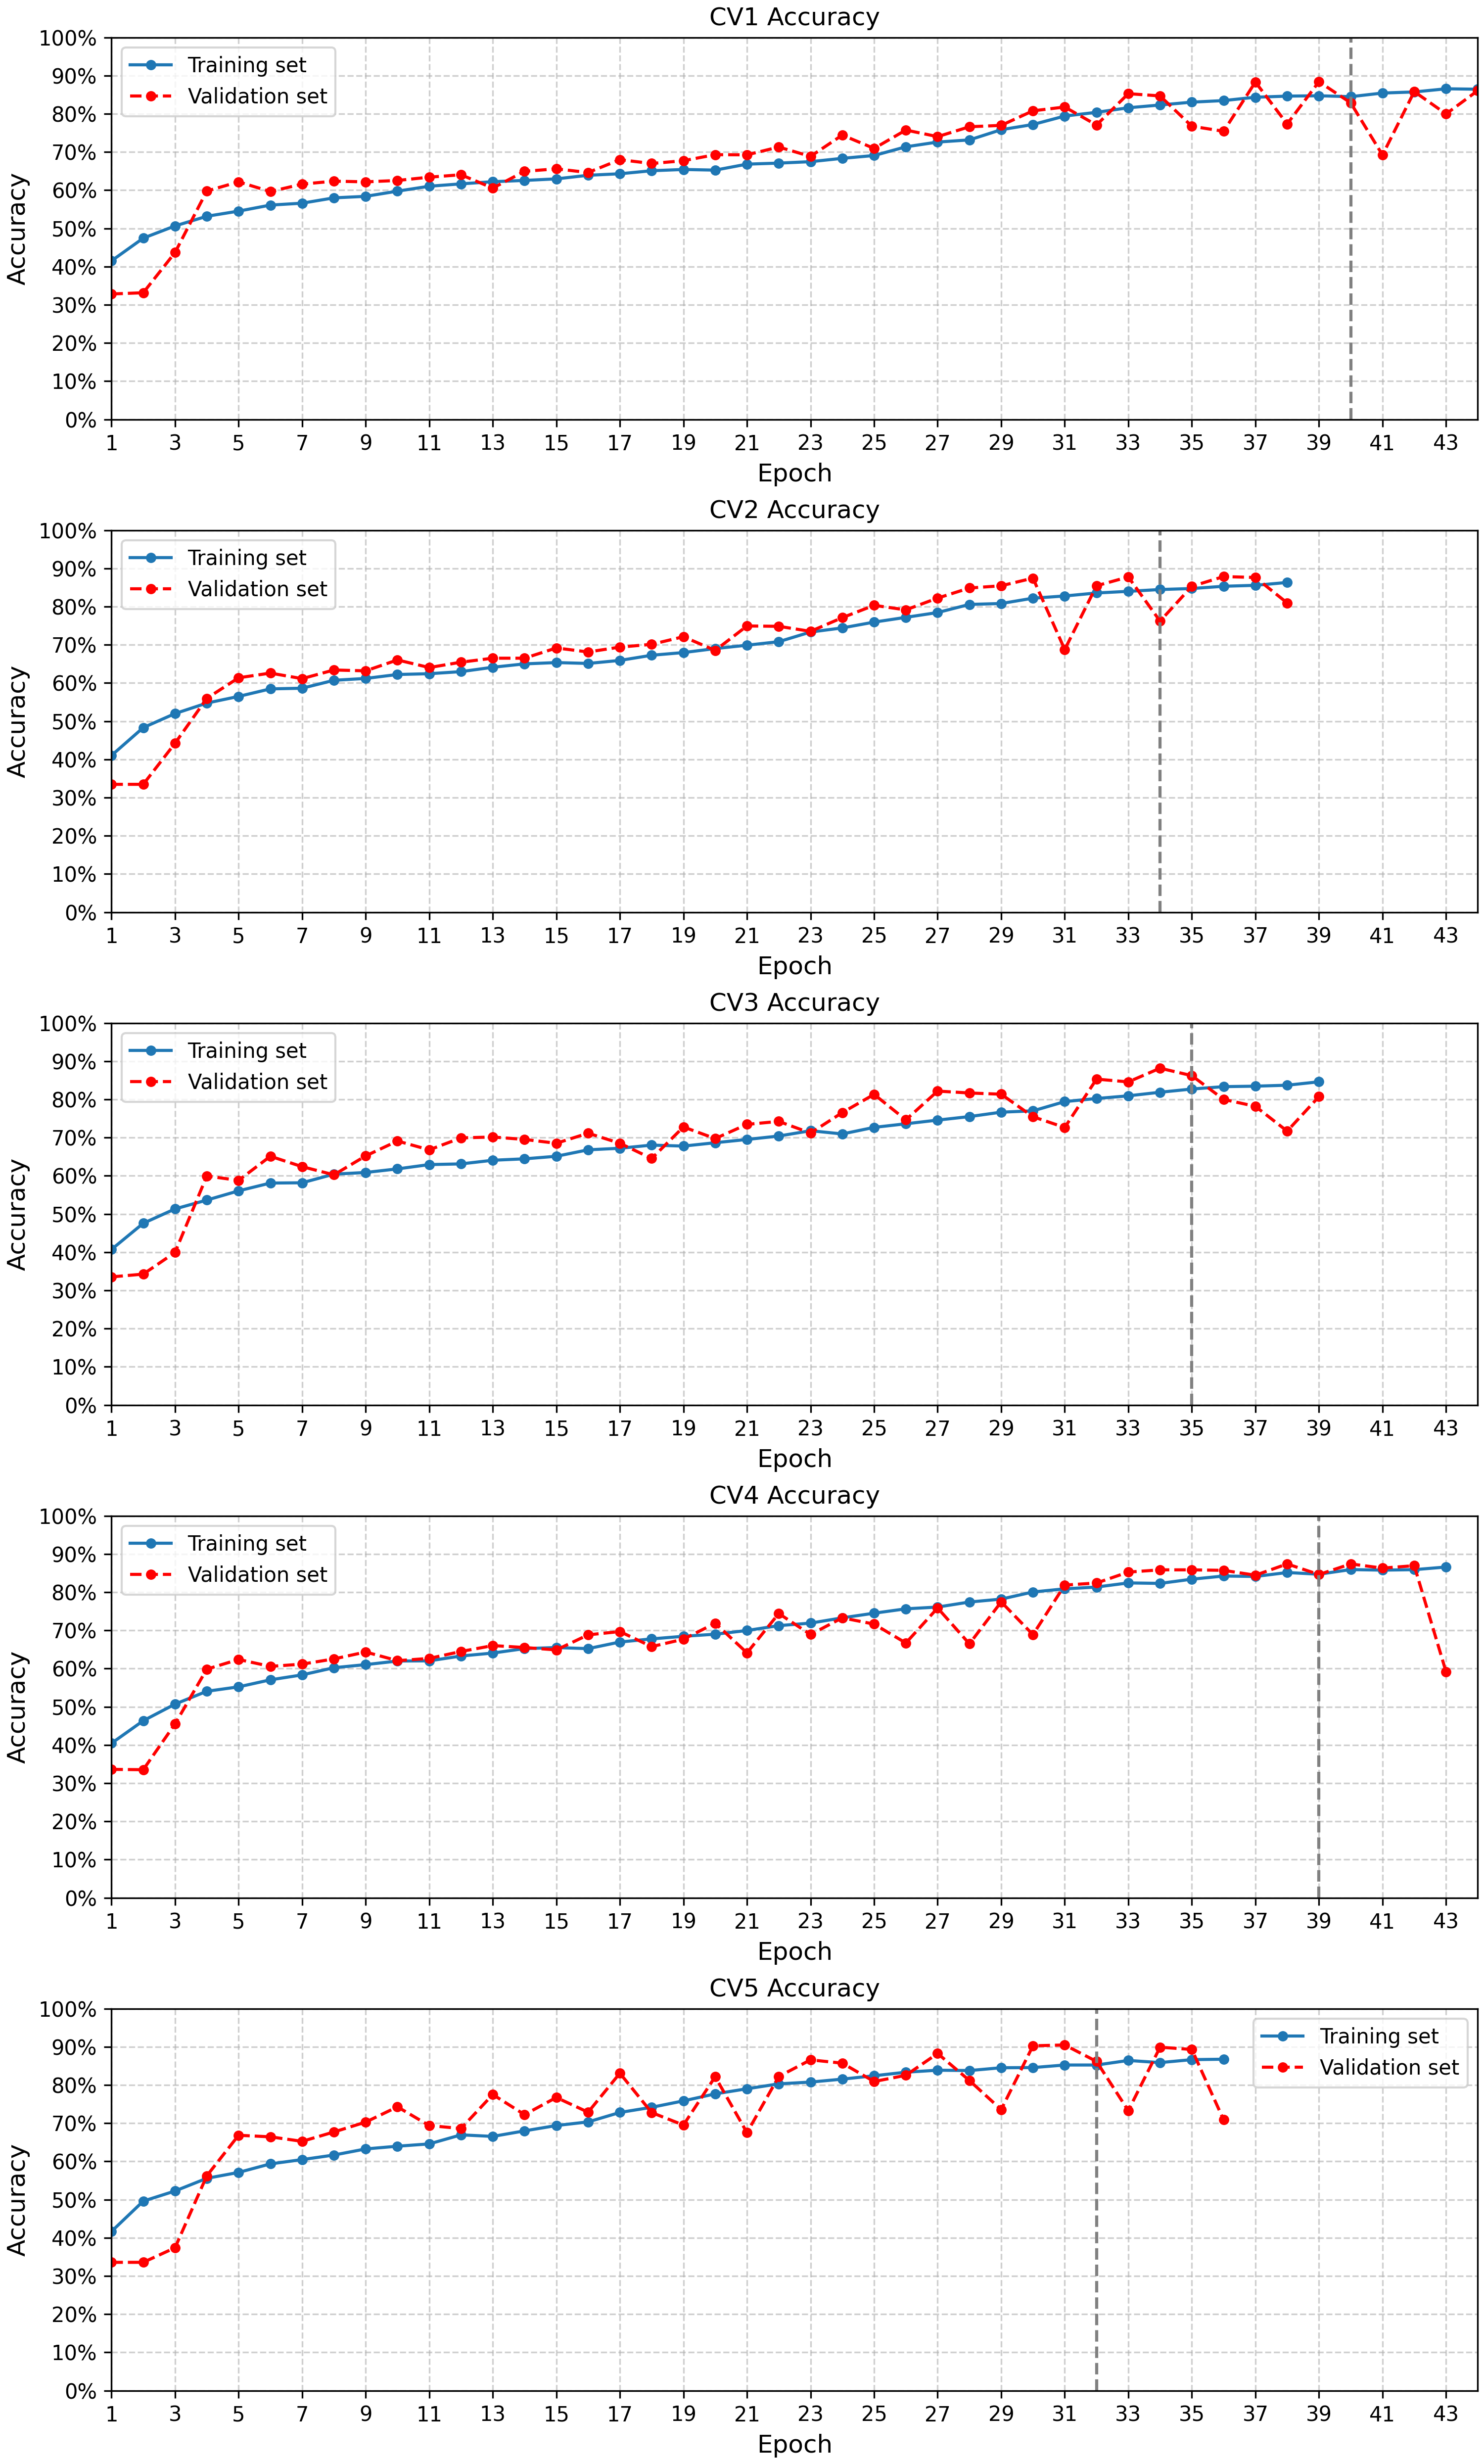
\includegraphics[width= 0.85\linewidth]{figures/bab4/akurasi_plotfix.png}
              \caption{Akurasi \textit{Training} Model}
              \label{Akurasi Training Model Terbaik}
          \end{figure}

          \begin{figure}[H]
              \centering
              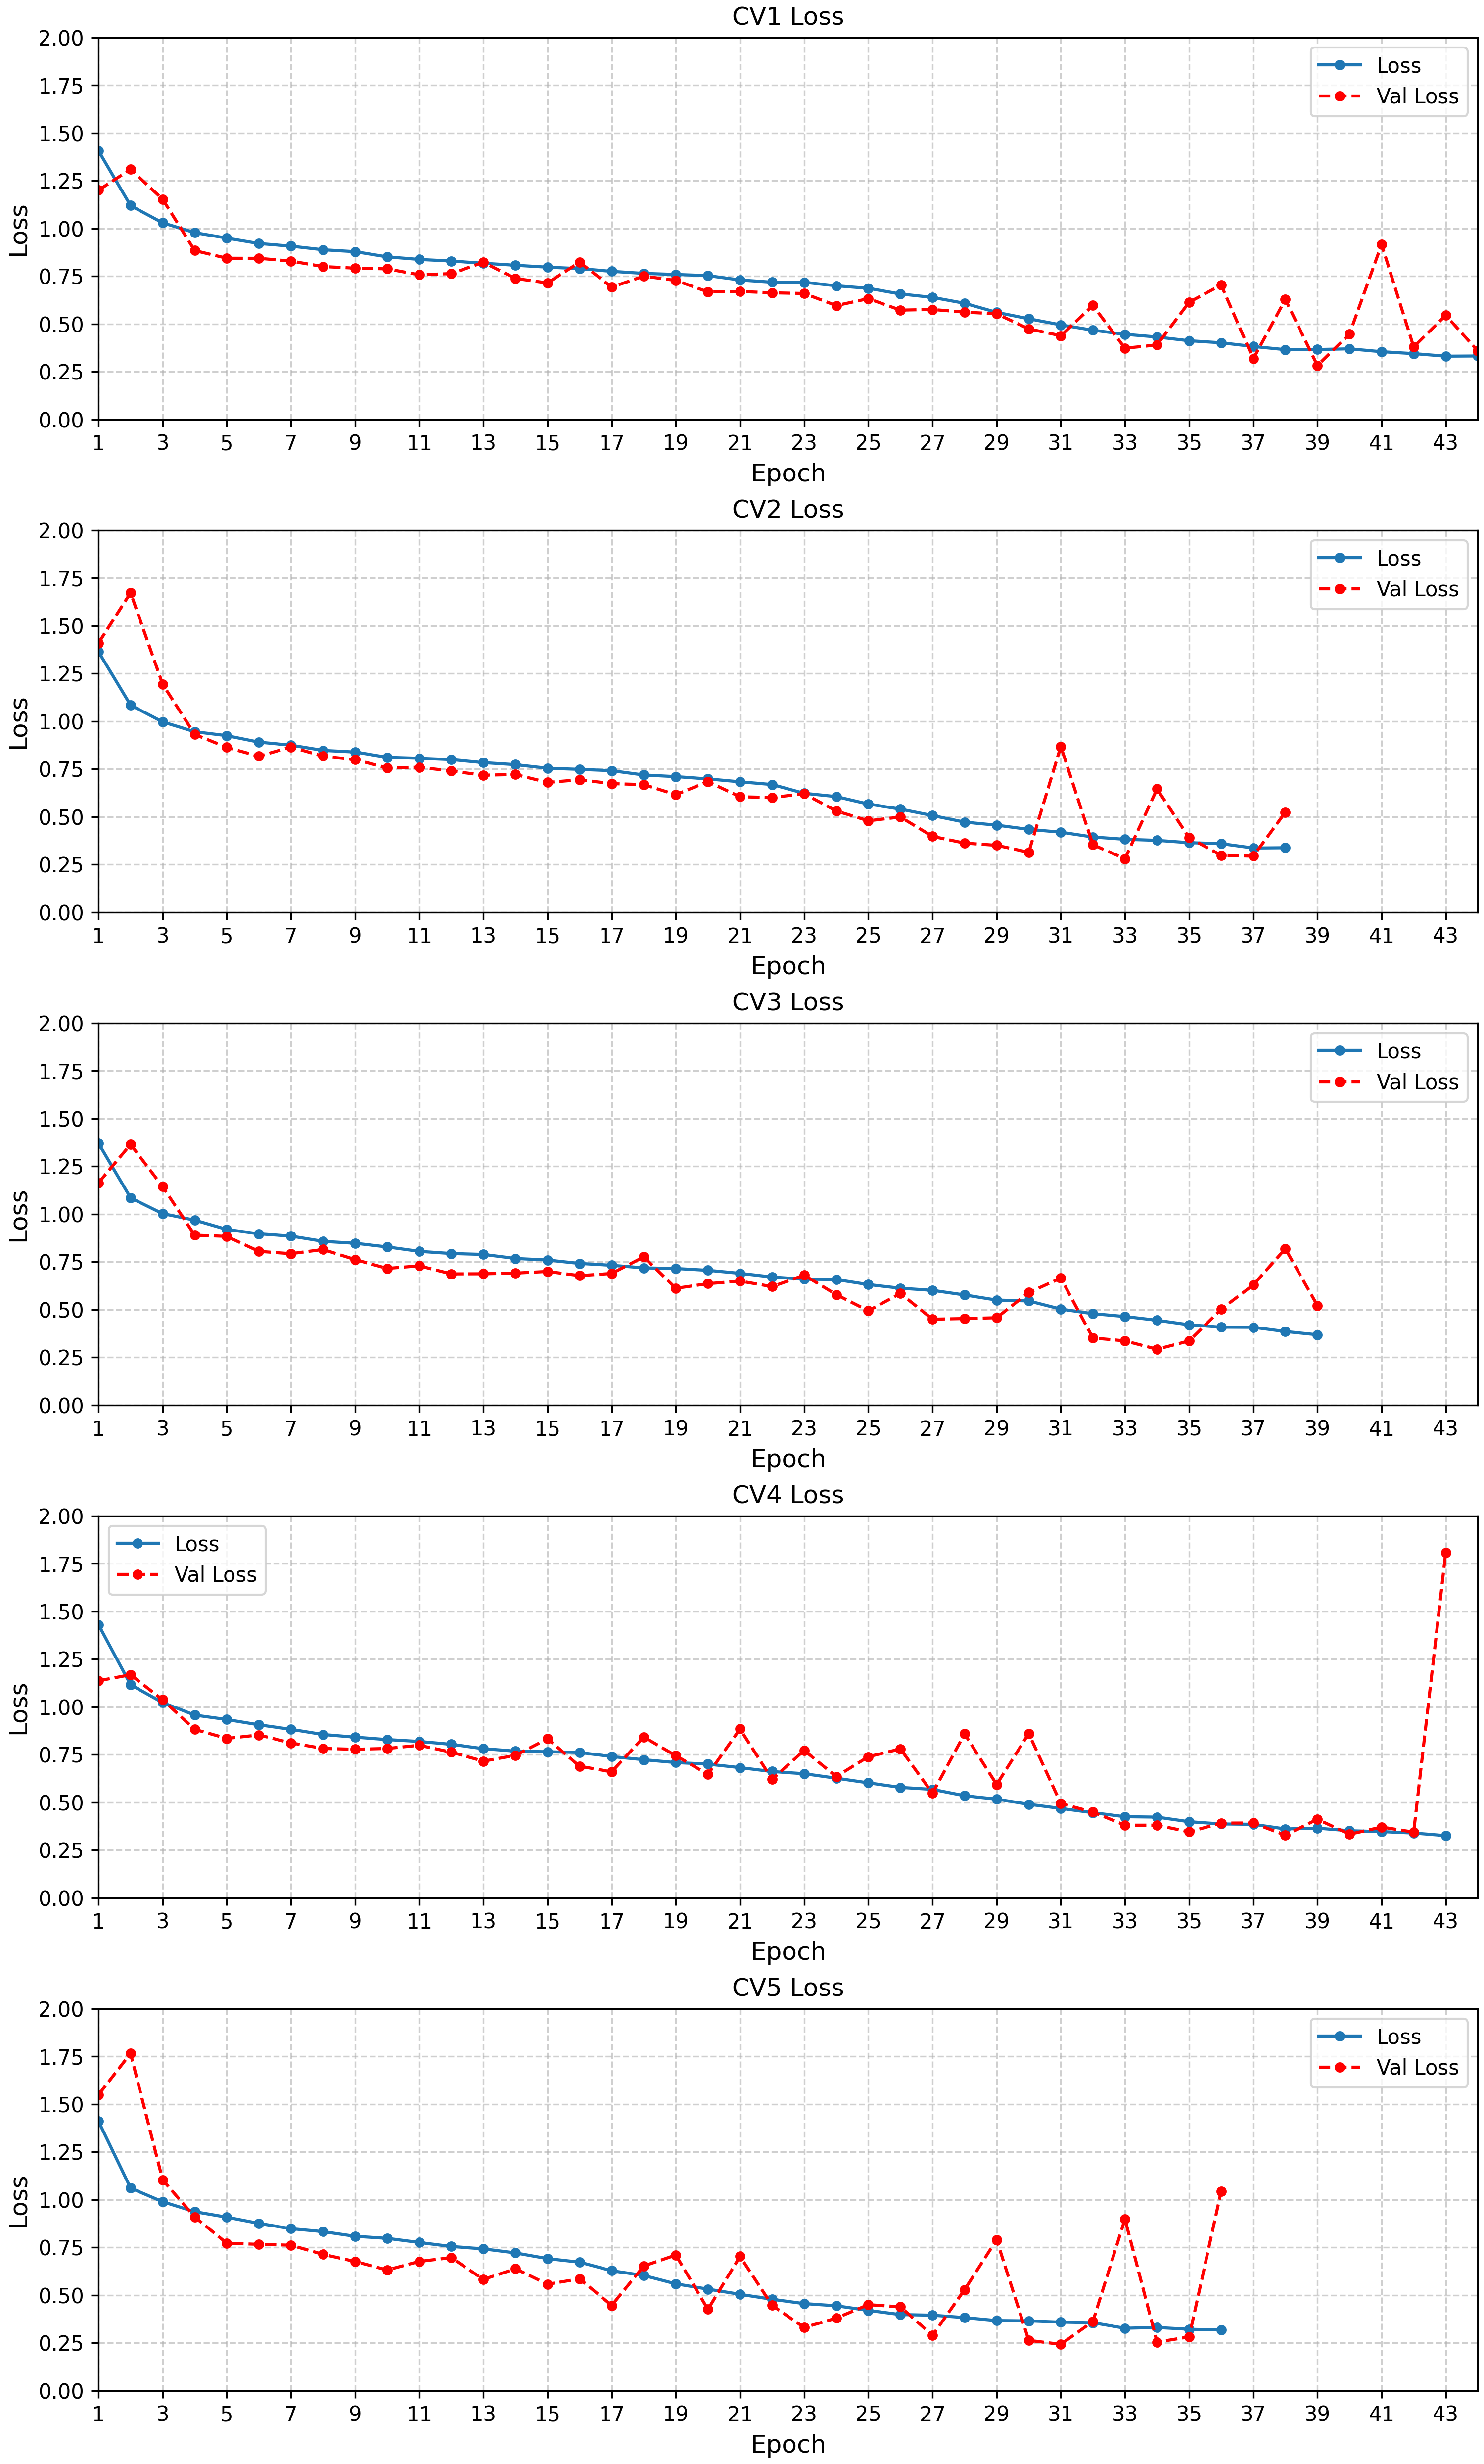
\includegraphics[width=0.85\linewidth]{figures/bab4/loss_plotfix.png}
              \caption{\textit{Loss Training} Model}
              \label{Loss Training Model Terbaik}
          \end{figure}

    Dapat dilihat akurasi dan \textit{loss} stabil di semua \textit{fold}, semakin tinggi nilai \textit{epoch} akurasi semakin meningkat dan akurasi di atas 90\%. Begitu juga dengan nilai \textit{loss} semakin tinggi \textit{epoch} semakin mengecil nilai \textit{loss} yang dihasilkan dan mendekati nilai nol.  Hal ini menunjukkan bahwa model mampu belajar dari data dan tidak hanya menghafal data pelatihan. Ini berarti model memiliki kinerja baik pada data baru yang tidak dilihat saat pelatihan.



  \subsection{Evaluasi Hasil}

        Pada tahap selanjutnya model di uji menggunakan data \textit{test} yang merupakan data baru yang tidak dilihat pada saat pelatihan. Hasil \textit{testing} model ditampilkan pada Gambar \ref{akurasi model terbaik} berikut.

          \begin{figure}[H]
              \centering
              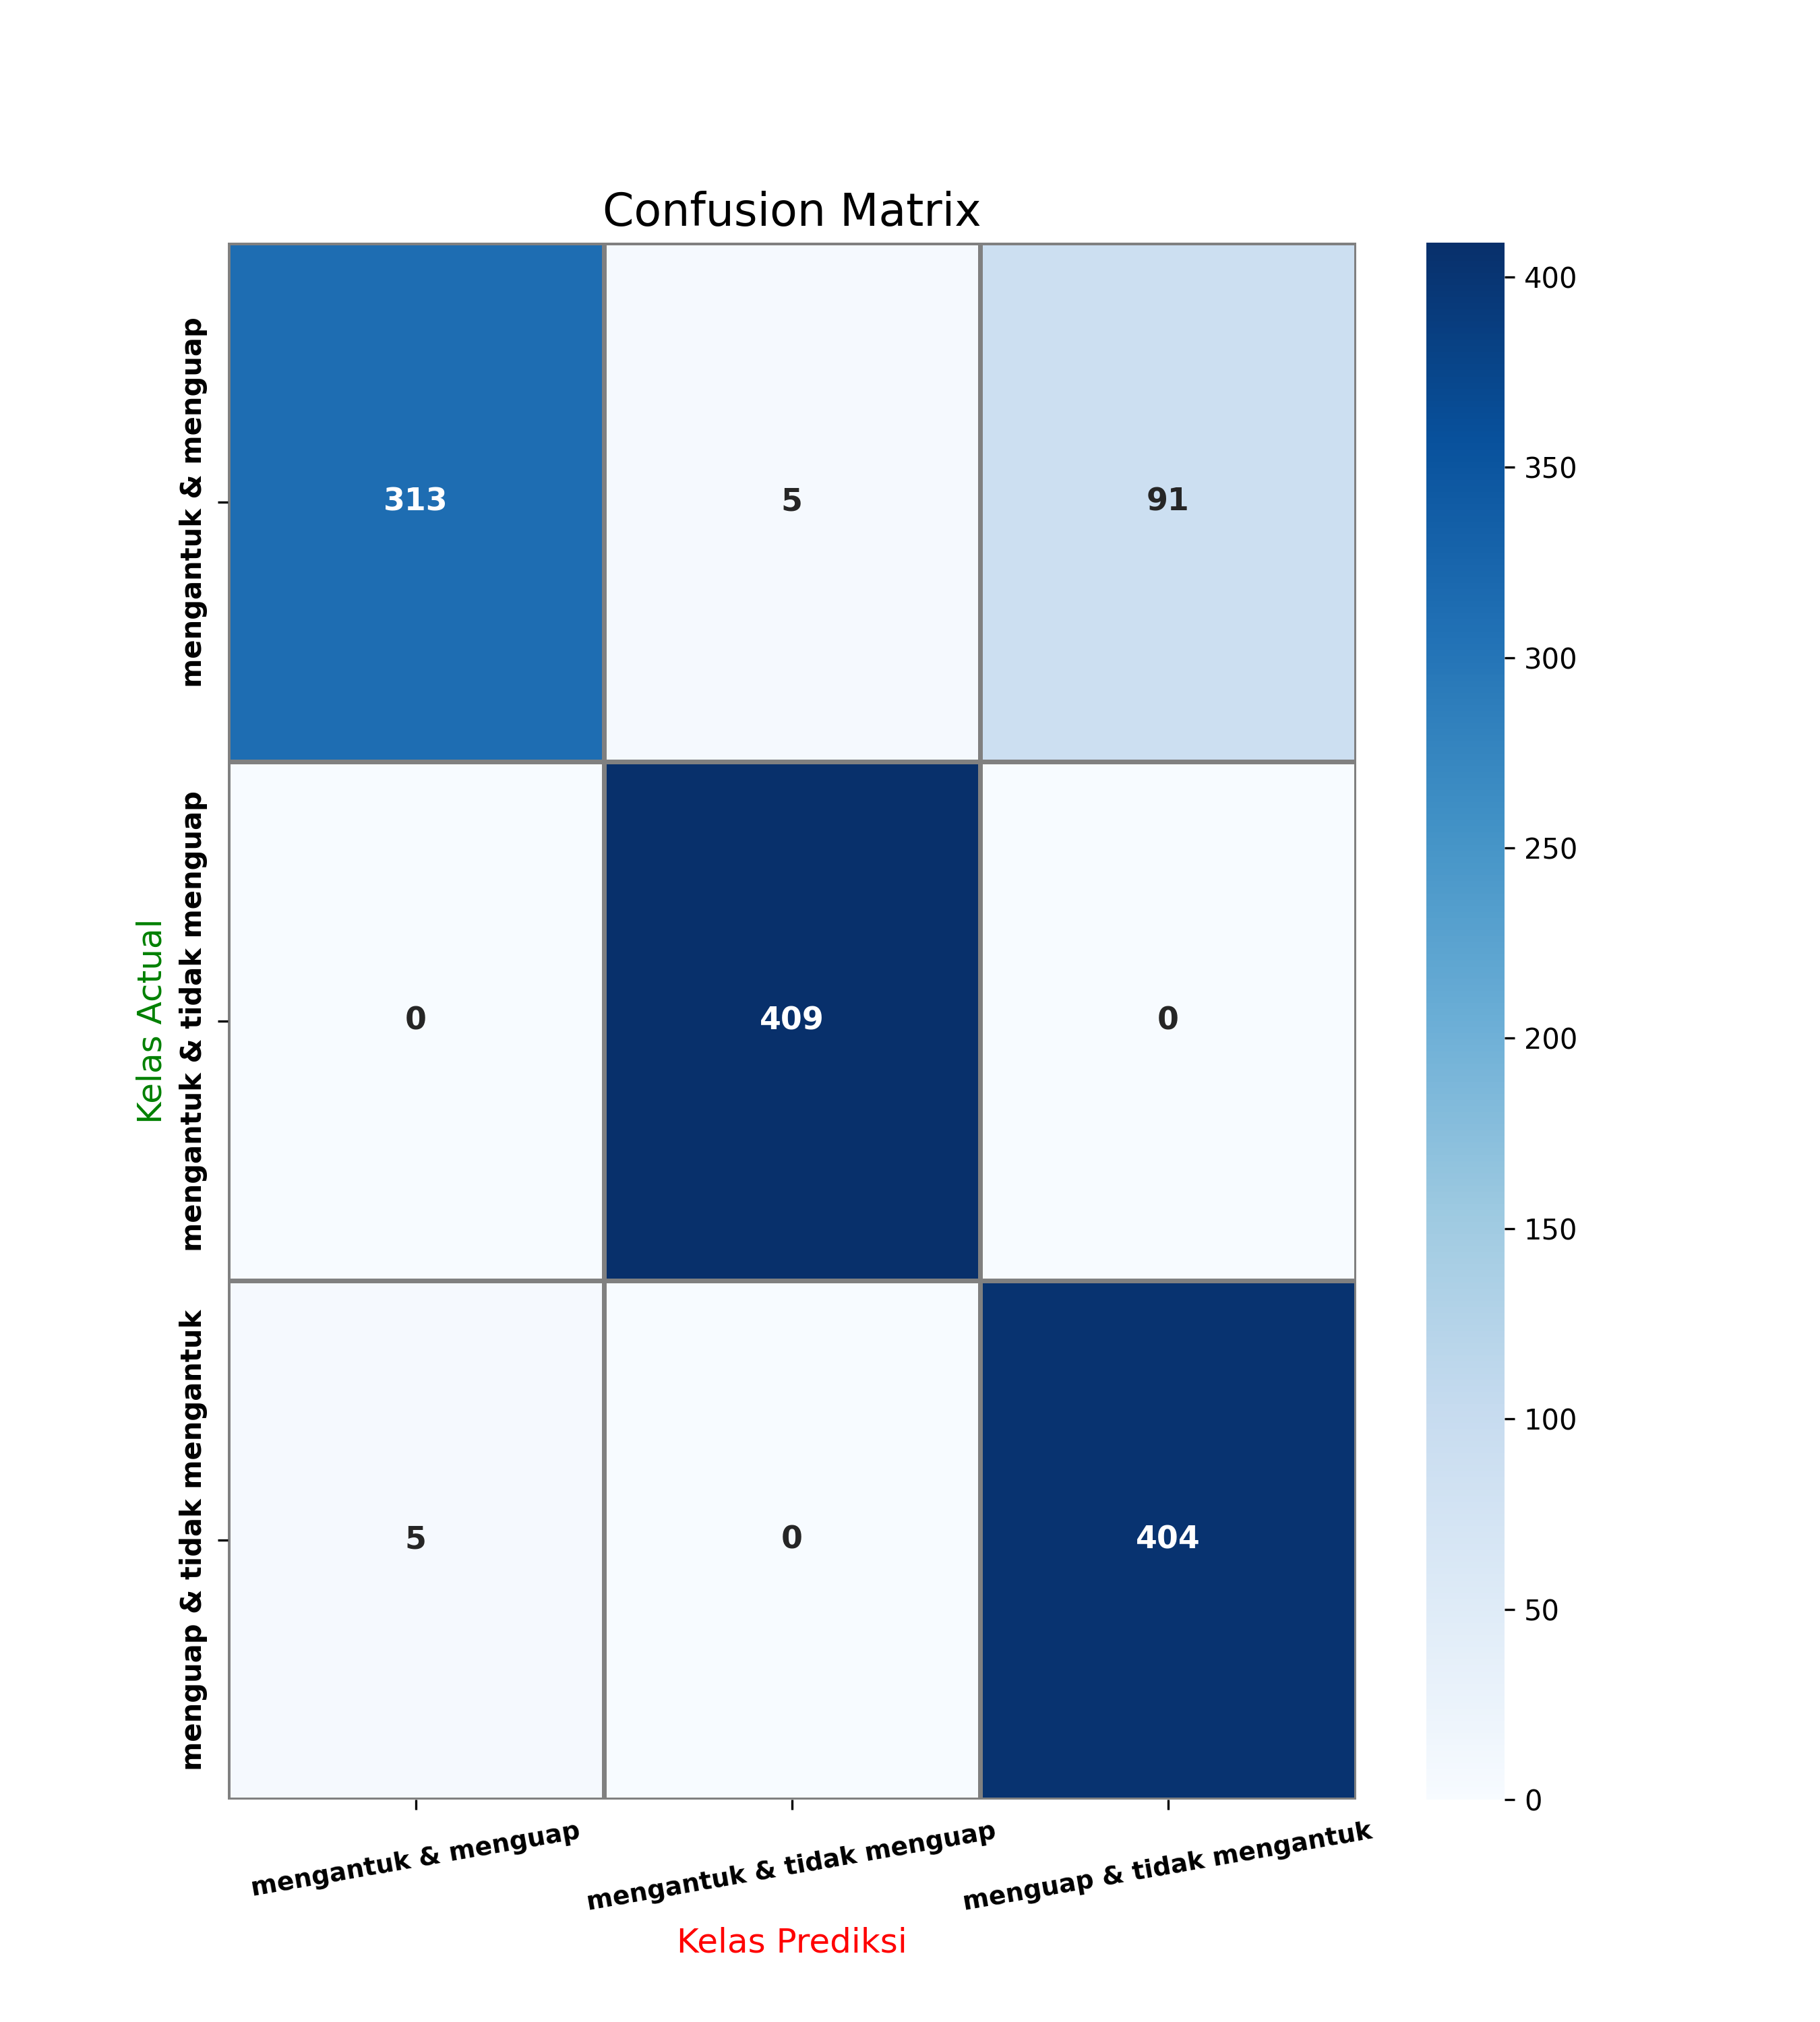
\includegraphics[width=0.75\linewidth]{figures/bab4/confusion matriks.png}
              \caption{Performa Matriks Model CNN}
              \label{akurasi model terbaik}
          \end{figure}

        Dapat dilihat dari hasil evaluasi menggunakan \textit{confusion matrix}. Nilai akurasi dan metriks yang dihasilkan tidak berbeda jauh dengan pengujian yang dilakukan sebelumnya. Hasil evaluasi ditampilkan pada Tabel \ref{Evaluasi Model} berikut.


        \begin{table}[H]
        \centering
        \caption{Evaluasi Model}
        \begin{tabular}{lccccc}
            \toprule
            \textbf{\textit{Kelas}} & \textbf{\textit{Recall}} & \textbf{\textit{Precision}} &\textbf{\textit{F1-Score}} & \textbf{\textit{Support }}\\
            
              & \textbf{(\%)} & \textbf{(\%)} & \textbf{(\%)} \\
            \midrule
            Mengantuk \& Menguap & 98.42 & 76.52 & 86.10 & 409 \\
            Mengantuk \& Tidak Menguap & 98.79 & 100.00 & 99.39 & 409 \\
            Menguap \& Tidak Mengantuk & 81.61 & 98.77 & 89.37 & 409 \\ \hline
            & & & & \\
            Accuracy & & & \textbf{91.76} & 1227 \\
            Average & 92.94 & 91.76 & 91.62 & 1227 \\
      
          
             \bottomrule
        \end{tabular}
        \label{Evaluasi Model}
    \end{table}

    Untuk hasil prediksi ditampilkan pada Gambar \ref{hasil prediksi} berikut.
         
          \begin{figure}[H]
              \centering
              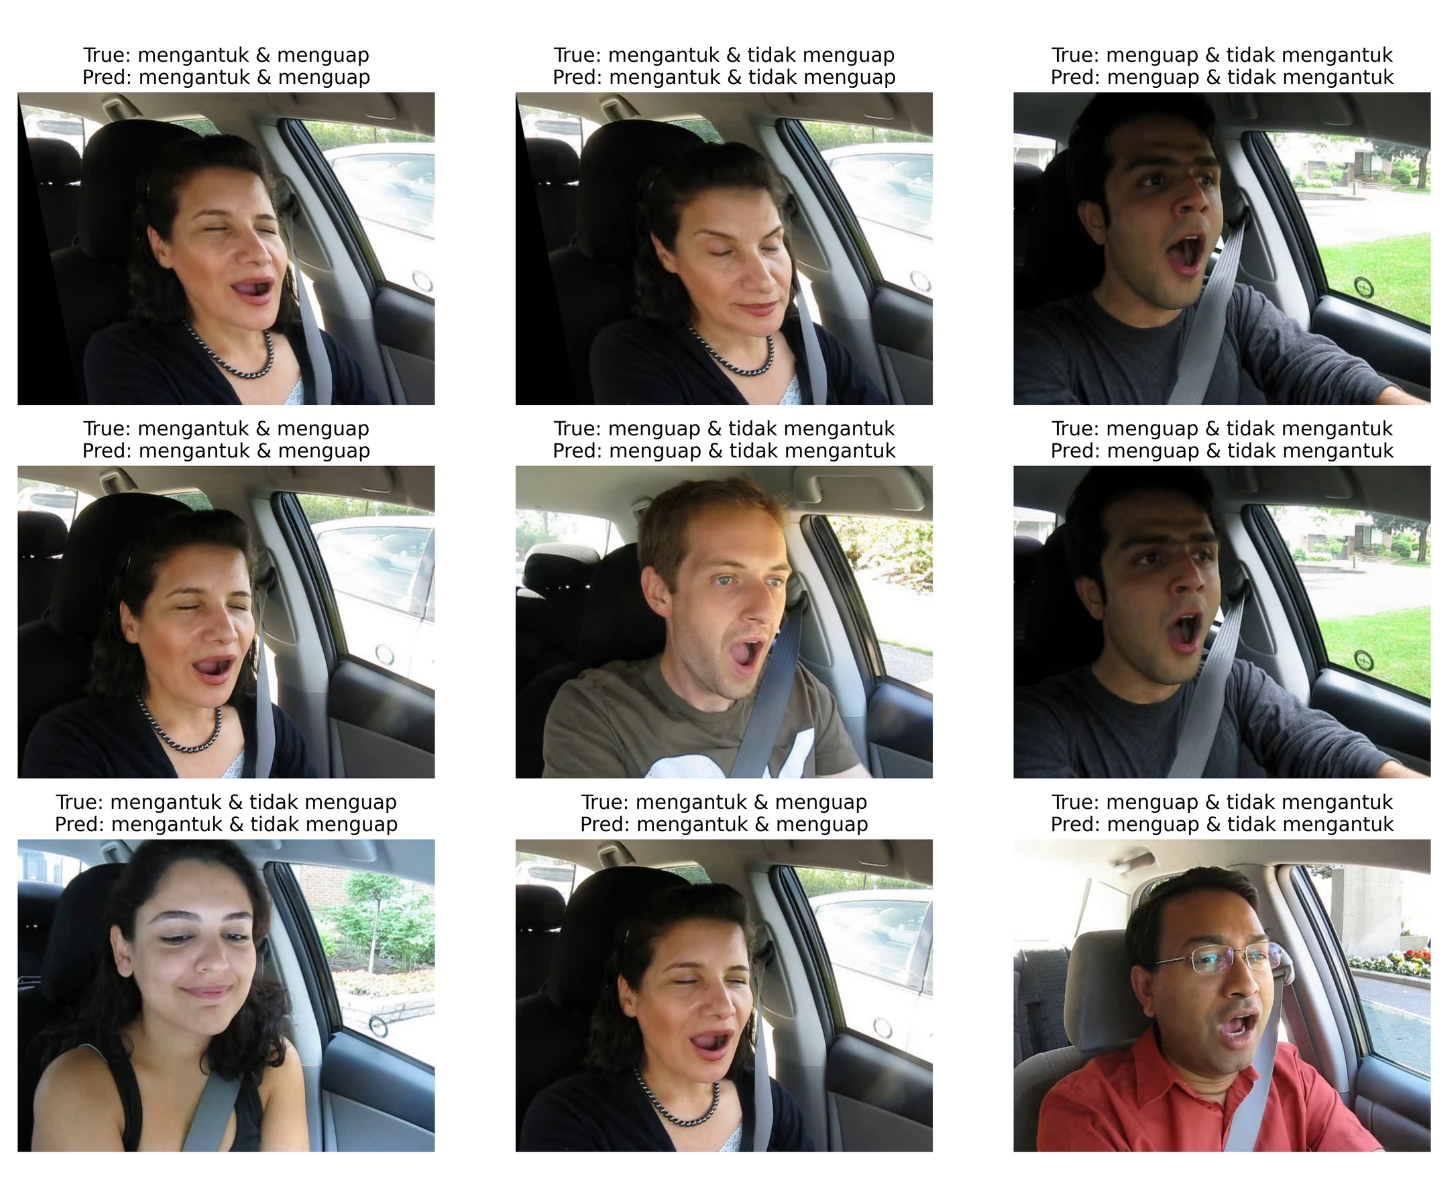
\includegraphics[width=1.0\linewidth]{figures/bab4/hasil_prediksi.png}
              \caption{Hasil prediksi}
              \label{hasil prediksi}
          \end{figure}

    
        
        
    Berdasarkan hasil percobaan yang telah dilakukan jika dibandingkan
     dengan penelitian sebelumnya yang dilakukan oleh Fiaz Majeed, dkk \cite{majeed2023detection}. Akurasi penelitian sebelumnya lebih tinggi dibandingkan penelitian ini, hal ini disebabkan adanya perbedaan segmentasi data, jumlah kelas dan metode yang dilakukan merupakan kombinasi antara CNN dan RNN. Ringkasan penelitian sebelumnya dapat dilihat pada Tabel \ref{Penelitian lama} berikut. 


    \begin{table}[H]
        \centering
        \caption{Penelitian Deteksi Kantuk Sebelumnya \cite{majeed2023detection}}
         \label{Penelitian lama}
        \begin{tabular}%{p{0.5cm}p{1.8cm}p{2.9cm}p{1.1cm}p{4.1cm}p{1cm}}
              {  >{\raggedright\arraybackslash}p{0.5cm} 
        >{\raggedright\arraybackslash}p{3 cm} 
        >{\raggedright\arraybackslash}p{2cm} 
        >{\raggedright\arraybackslash}p{5.0cm} 
        >{\raggedright\arraybackslash}p{1.0cm}}
    
            \hline
            \textbf{No}  & \textbf{Topik} &\textbf{ Metode} & \textbf{Hasil} & \textbf{Tahun} \\
            
            \hline
             1 
            &
            \textit{Detection of Drowsiness among Drivers Using Novel Deep Convolutional Neural Network Model}
            & 
            CNN \& RNN
            &
            
             Segmentasi data dilakukan dengan nilai MAR, dengan kelas yang diterapkan berupa \textit{binary class}. Eksperimen menunjukkan bahwa model mencapai akurasi rata-rata 96,69\% .
            &
            2023 \\   
            \\

             \hline

        \end{tabular}
    \end{table}


    Penelitian ini menghasilkan akurasi yang lebih rendah dibandingkan sebelumnya yaitu sebesar 91.76 \%. Hal ini terjadi karena pada penelitian ini menggunakan segmentasi data dengan nilai EAR dan MAR sedangkan sebelumnya hanya MAR. Penelitian ini juga menggunakan \textit{Multi-Class} sehingga jumlah model lebih sulit melakukan klasifikasi.

        \begin{table}[H]
        \centering
        \caption{Penelitian Deteksi Kantuk Baru}
         \label{Penelitian lama}
        \begin{tabular}%{p{0.5cm}p{1.8cm}p{2.9cm}p{1.1cm}p{4.1cm}p{1cm}}
              {  >{\raggedright\arraybackslash}p{0.5cm} 
        >{\raggedright\arraybackslash}p{3 cm} 
        >{\raggedright\arraybackslash}p{2cm} 
        >{\raggedright\arraybackslash}p{5.0cm} 
        >{\raggedright\arraybackslash}p{1.0cm}}
    
            \hline
            \textbf{No}  & \textbf{Topik} &\textbf{ Metode} & \textbf{Hasil} & \textbf{Tahun} \\
            
            \hline
             1
            & 
            Deteksi Kantuk Pengendara Mobil Menggunkan \textit{Convolutional Neural Networks} (CNN)

            & 
            CNN
            &
            Segmentasi data dilakukan dengan nilai EAR dan MAR, dengan kelas yang diterapkan berupa \textit{multi class} dengan hasil akurasi sebesar 91.76\%

            &
            2024 \\

             \hline

        \end{tabular}
    \end{table}


    \chapter{Penutup}

\section{Kesimpulan}

    \begin{enumerate}
        \item Deteksi kantuk pada pengendara di di klasifikasi berdasarkan nilai \textit{Eye Aspect Ratio} (EAR) dan \textit{Mouth Aspect Ratio} (MAR).
        Terdapat tiga kelas yang dilatih menggunakan \textit{Convolutional Neural Network} (CNN) untuk mengidentifikasi pola pengendara menggunakan seperti ’mengantuk dan menguap’, ’mengantuk tidak menguap’ dan ’menguap tidak mengantuk’, ketiga kelas tersebut merupakan kombinasi antara parameter EAR \& MAR.
        
        \item Performa terbaik model diperoleh pada skenario pengujian parameter dengan nilai \textit{learning rate} sebesar 0,0001, \textit{activation} ReLU dan \textit{Optimizer} SGD. Perubahan \textit{learning rate} dari 0.01 menjadi 0.001 mengalami peningkatan akurasi yang signifikan. Pada \textit{activation softmax} tidak mengalami perubahan yang cukup berarti pada beberapa \textit{learning rate}, sehingga buruk dalam melakukan klasifikasi. Setelah dilakukan beberapa pengujian parameter, model dengan parameter terbaik mencapai nilai akurasi sebesar 92.97\%, \textit{precision} sebesar 93.32\%, \textit{recall} sebesar 92.72\%, dan \textit{F1-Score} sebesar 92.98\%.
    \end{enumerate}


\section{Saran}

Berdasarkan penelitian yang telah dilakukan, dengan deteksi kantuk dapat menggunakan metode \textit{Convolutional Neural Network} (CNN) mempertimbangkan nilai parameter \textit{Eye Aspect Ratio} (EAR) dan \textit{Mouth Aspect Ratio} (MAR) untuk ekstraksi data video menjadi gambar pada kelas yang ditentukan. Untuk pencarian model CNN terbaik, parameter yang di \textit{tuning} adalah \textit{learning rate}, \textit{activation} dan \textit{optimizer}. Penelitian selanjutnya disarankan untuk menggunakan nilai EAR dan MAR yang berbeda untuk ektraksi data, serta menggunakan metode lain untuk melakukan \textit{tuning} parameter.









    %----------------------------------------------------------------%

    % Daftar pustaka
    \renewcommand{\bibname}{Daftar Pustaka}
    \phantomsection% 
    \addcontentsline{toc}{chapter}{Daftar Pustaka}
    \printbibliography
    

    % Index
    \appendix

    \addcontentsline{toc}{part}{Lampiran}
    \part*{Lampiran}

    \chapter{Perhitungan Manual Parameter CNN}



\begin{table}[H]
    \centering
    \scriptsize
    %\caption{Desain Arsitektur}
    \renewcommand{\arraystretch}{1.5}
    \begin{tabular}{p{1cm}p{4.5cm}p{4cm}p{2.5cm}}
    \hline
    \textbf{No} & \textbf{Layer (type)}   & \textbf{Output Shape} & \textbf{Parameters}  \\ \hline
    
    1 & conv2d                   & (64, 64, 32)   & 896     \\ 
    2 & conv2d\_1                & (64, 64, 32)   & 9248    \\ 
    3 & batch\_normalization     & (64, 64, 32)   & 128     \\ 
    4 & max\_pooling2d           & (32, 32, 32)   & 0       \\ 
    5 & conv2d\_2                & (32, 32, 64)   & 18496   \\ 
    6 & conv2d\_3                & (32, 32, 64)   & 36928   \\ 
    7 & batch\_normalization\_1  & (32, 32, 64)   & 256     \\ 
    8 & max\_pooling2d\_1        & (16, 16, 64)   & 0       \\ 
    9 & conv2d\_4                & (16, 16, 128)  & 73856   \\ 
    10 & conv2d\_5                & (16, 16, 128)  & 147584  \\ 
    11 & batch\_normalization\_2  & (16, 16, 128)  & 512     \\ 
    12 & max\_pooling2d\_2        & (8, 8, 128)    & 0       \\ 
    13 & dropout                  & (8, 8, 128)    & 0       \\ 
    14 & flatten                  & (8192)         & 0       \\ 
    15 & dense                    & (256)          & 2097408 \\ 
    16 & dense\_1                 & (3)            & 771     \\ \hline
    \end{tabular}
\end{table}



\begin{enumerate}
    \item \textbf{conv2d}
    \[
    \text{Parameter} = (\text{ukuran filter} \times \text{ukuran filter} \times \text{jumlah channel input} + 1) \times \text{jumlah filter}
    \]
    \[
    = (3 \times 3 \times 3 + 1) \times 32 = (27 + 1) \times 32 = 28 \times 32 = 896
    \]

    \item \textbf{conv2d\_1}
    \[
    \text{Parameter} = (3 \times 3 \times 32 + 1) \times 32 = (288 + 1) \times 32 = 289 \times 32 = 9248
    \]

    \item \textbf{batch\_normalization}
    \[
    \text{Parameter} = 2 \times \text{jumlah channel output} = 2 \times 32 = 64 + 64 = 128
    \]

    \item \textbf{max\_pooling2d}
    \[
    \text{Parameter} = 0
    \]

    \item \textbf{conv2d\_2}
    \[
    \text{Parameter} = (3 \times 3 \times 32 + 1) \times 64 = (288 + 1) \times 64 = 289 \times 64 = 18496
    \]

    \item \textbf{conv2d\_3}
    \[
    \text{Parameter} = (3 \times 3 \times 64 + 1) \times 64 = (576 + 1) \times 64 = 577 \times 64 = 36928
    \]

    \item \textbf{batch\_normalization\_1}
    \[
    \text{Parameter} = 2 \times \text{jumlah channel output} = 2 \times 64 = 128 + 128 = 256
    \]

    \item \textbf{max\_pooling2d\_1}
    \[
    \text{Parameter} = 0
    \]

    \item \textbf{conv2d\_4}
    \[
    \text{Parameter} = (3 \times 3 \times 64 + 1) \times 128 = (576 + 1) \times 128 = 577 \times 128 = 73856
    \]

    \item \textbf{conv2d\_5}
    \[
    \text{Parameter} = (3 \times 3 \times 128 + 1) \times 128 = (1152 + 1) \times 128 = 1153 \times 128 = 147584
    \]

    \item \textbf{batch\_normalization\_2}
    \[
    \text{Parameter} = 2 \times \text{jumlah channel output} = 2 \times 128 = 256 + 256 = 512
    \]

    \item \textbf{max\_pooling2d\_2}
    \[
    \text{Parameter} = 0
    \]

    \item \textbf{dropout}
    \[
    \text{Parameter} = 0
    \]

    \item \textbf{flatten}
    \[
    \text{Parameter} = 0
    \]

    \item \textbf{dense}
    \[
    \text{Parameter} = (\text{jumlah neuron input} + 1) \times \text{jumlah neuron output}
    \]
    \[
    = (8192 + 1) \times 256 = 8193 \times 256 = 2097408
    \]

    \item \textbf{dense\_1}
    \[
    \text{Parameter} = (256 + 1) \times 3 = 257 \times 3 = 771
    \]
\end{enumerate}

\subsection*{Total Jumlah Parameter}

\[
896 + 9248 + 128 + 0 + 18496 + 36928 + 256 + 0 + 73856 + 147584 \]\\
\[ + 512 + 0 + 0 + 0 + 2097408 + 771 = 2373183
\]

Jadi, total jumlah parameter pada CNN ini adalah 2,373,183.

    \chapter{Perhitungan Manual Aktivasi \textit{Sigmoid, Softmax}, dan ReLU}

\subsection*{1. \textit{Sigmoid}}
Fungsi aktivasi \textit{sigmoid} mendefinisikan output sebagai:
\[
\sigma(x) = \frac{1}{1 + e^{-x}}
\]

Contoh: Misalkan \( x = 1.5 \).

Langkah-langkah:
\begin{enumerate}
    \item Hitung \( e^{-x} \):
    \[
    e^{-1.5} \approx 0.2231
    \]

    \item Tambahkan 1 ke hasil tersebut:
    \[
    1 + 0.2231 = 1.2231
    \]

    \item Hitung kebalikan (1 per hasil tersebut):
    \[
    \frac{1}{1.2231} \approx 0.8176
    \]
\end{enumerate}

Jadi, nilai aktivasi \textit{sigmoid} untuk \( x = 1.5 \) adalah sekitar \( 0.8176 \).

\subsection*{2. \textit{Softmax}}
Fungsi aktivasi \textit{softmax} menghitung probabilitas dari beberapa kelas. Untuk vektor input \(\mathbf{x} = [x_1, x_2, x_3, \ldots, x_n]\), fungsi \textit{softmax} mendefinisikan \textit{output} sebagai:
\[
\sigma(x_i) = \frac{e^{x_i}}{\sum_{j=1}^{n} e^{x_j}}
\]

Contoh: Misalkan \(\mathbf{x} = [2.0, 1.0, 0.1]\).

Langkah-langkah:
\begin{enumerate}
    \item Hitung \( e^{x_i} \) untuk setiap elemen:
    \[
    e^{2.0} \approx 7.389
    \]
    \[
    e^{1.0} \approx 2.718
    \]
    \[
    e^{0.1} \approx 1.105
    \]

    \item Hitung jumlah semua hasil eksponensial:
    \[
    7.389 + 2.718 + 1.105 = 11.212
    \]

    \item Hitung setiap probabilitas dengan membagi hasil eksponensial masing-masing elemen dengan jumlah total:
    \[
    \sigma(x_1) = \frac{7.389}{11.212} \approx 0.659
    \]
    \[
    \sigma(x_2) = \frac{2.718}{11.212} \approx 0.242
    \]
    \[
    \sigma(x_3) = \frac{1.105}{11.212} \approx 0.099
    \]
\end{enumerate}

Jadi, hasil \textit{softmax} untuk \(\mathbf{x} = [2.0, 1.0, 0.1]\) adalah sekitar \([0.659, 0.242, 0.099]\).

\subsection*{3. ReLU (\textit{Rectified Linear Unit})}
Fungsi aktivasi ReLU mendefinisikan output sebagai:
\[
\text{ReLU}(x) = \max(0, x)
\]

Contoh: Misalkan \( x = -2.0, 1.0, 0.0, 3.5 \).

Langkah-langkah:
\begin{enumerate}
    \item Untuk \( x = -2.0 \):
    \[
    \text{ReLU}(-2.0) = \max(0, -2.0) = 0
    \]

    \item Untuk \( x = 1.0 \):
    \[
    \text{ReLU}(1.0) = \max(0, 1.0) = 1.0
    \]

    \item Untuk \( x = 0.0 \):
    \[
    \text{ReLU}(0.0) = \max(0, 0.0) = 0
    \]

    \item Untuk \( x = 3.5 \):
    \[
    \text{ReLU}(3.5) = \max(0, 3.5) = 3.5
    \]
\end{enumerate}

Jadi, hasil ReLU untuk \( x = [-2.0, 1.0, 0.0, 3.5] \) adalah \([0, 1.0, 0, 3.5]\).



\chapter{Perhitungan Manual Optimizer Adam dan SGD}
\subsection*{1. \textit{Stochastic Gradient Descent} (SGD)}

\subsection*{Persamaan}
\begin{align}
    W & = \omega - \eta \cdot \nabla Q_i(\omega) \\
    Q(\omega) & = \ln\left(\sum_i Q_i(\omega)\right) \\
    \nabla Q(\omega) & = \ln\left(\sum_i \nabla Q_i(\omega)\right)
\end{align}



\subsection*{Keterangan:}
\begin{itemize}
    \item \( W \): Parameter model yang akan diperbarui.
    \item \( \omega \): Nilai parameter \( W \) saat ini.
    \item \( \eta \): Learning rate.
    \item \( Q_i(\omega) \): Nilai fungsi \( Q_i \) untuk contoh data ke-i.
    \item \( Q(\omega) = \ln\left(\sum_i Q_i(\omega)\right) \).
    \item \( \nabla Q(\omega) = \ln\left(\sum_i \nabla Q_i(\omega)\right) \).
\end{itemize}


\subsection*{Contoh Perhitungan}
Misalkan kita memiliki dua contoh data (\( i = 1, 2 \)), dengan:
\begin{itemize}
    \item Nilai parameter saat ini: \( \omega = 1.0 \)
    \item Learning rate: \( \eta = 0.1 \)
    \item Fungsi \( Q_1(\omega) = \omega^2 \) dan \( Q_2(\omega) = 2\omega \)
\end{itemize}

Langkah-langkah perhitungan manual:

1. Hitung nilai \( Q_i(\omega) \) untuk \( \omega = 1.0 \):
   \begin{align*}
       Q_1(1.0) & = (1.0)^2 = 1.0 \\
       Q_2(1.0) & = 2 \cdot 1.0 = 2.0
   \end{align*}

2. Hitung nilai \( Q(\omega) \):
   \[
   Q(\omega) = \ln\left(Q_1(\omega) + Q_2(\omega)\right) = \ln(1.0 + 2.0) = \ln(3.0)
   \]

3. Hitung gradien \( \nabla Q_i(\omega) \):
   \begin{align*}
       \nabla Q_1(\omega) & = \frac{d}{d\omega}(\omega^2) = 2\omega \\
       \nabla Q_2(\omega) & = \frac{d}{d\omega}(2\omega) = 2
   \end{align*}
   Jadi, untuk \( \omega = 1.0 \):
   \begin{align*}
       \nabla Q_1(1.0) & = 2 \cdot 1.0 = 2 \\
       \nabla Q_2(1.0) & = 2
   \end{align*}

4. Hitung gradien \( \nabla Q(\omega) \):
   \[
   \nabla Q(\omega) = \ln\left(\nabla Q_1(\omega) + \nabla Q_2(\omega)\right) = \ln(2 + 2) = \ln(4)
   \]

5. Pembaruan parameter \( W \):
   \begin{align*}
       W & = \omega - \eta \cdot \nabla Q(\omega) \\
       & = 1.0 - 0.1 \cdot \ln(4)
   \end{align*}
   Menghitung nilai \( \ln(4) \approx 1.386 \):
   \[
   W = 1.0 - 0.1 \cdot 1.386 = 1.0 - 0.1386 = 0.8614
   \]

\subsection*{Kesimpulan}
Parameter model \( W \) setelah satu iterasi pembaruan menggunakan SGD adalah \( W \approx 0.8614 \).

\vspace{3 cm}


\section*{1. \textit{Adaptive Moment Estimation } (Adam)}

\subsection*{Persamaan:}
    \begin{equation}
    \begin{aligned}
        x_t &= \delta_1 \cdot x_{t-1} - (1 - \delta_1) \cdot g_t \\
        y_t &= \delta_2 \cdot y_{t-1} - (1 - \delta_2) \cdot g_t^2 \\
        \Delta \omega_t &= -\eta \frac{x_t}{\sqrt{y_t + \epsilon}} \cdot g_t \\
        \omega_{t+1} &= \omega_t + \Delta \omega_t
    \end{aligned}
    \label{Adam}
    \end{equation}

 \textbf{Keterangan:}

    \begin{align*}
    x_t &: \text{Estimasi pertama dari rata-rata gradien pada iterasi ke-t}\\
    y_t &: \text{Estimasi kedua dari rata-rata gradien kedua pada iterasi ke-t}\\
    \omega_t &: \text{\textit{Learning rate} yang disesuaikan pada iterasi ke-t}\\
    g_t &: \text{Gradien dari parameter pada iterasi ke-t}\\
    \delta_1, \delta_2 &: \text{Hyperparameter untuk estimasi pertama dan kedua terhadap gradien baru}\\
    \eta &: \text{\textit{Learning rate}}\\
\end{align*}



\subsection*{Diberikan:}
\begin{itemize}
    \item $\delta_1$: Hyperparameter untuk estimasi pertama dari rata-rata gradien (biasanya sekitar 0.9)
    \item $\delta_2$: Hyperparameter untuk estimasi kedua dari rata-rata gradien kedua (biasanya sekitar 0.999)
    \item $\eta$: Learning rate (biasanya nilai kecil seperti 0.001)
    \item $\epsilon$: Nilai kecil untuk menghindari pembagian dengan nol (biasanya $10^{-8}$)
    \item $g_t$: Gradien dari parameter pada iterasi ke-t
\end{itemize}



\subsection*{Contoh Perhitungan:}
Misalkan nilai awal sebagai berikut:
\begin{itemize}
    \item $x_0 = 0$
    \item $y_0 = 0$
    \item $\omega_0 = 0.5$
    \item $\delta_1 = 0.9$
    \item $\delta_2 = 0.999$
    \item $\eta = 0.001$
    \item $\epsilon = 10^{-8}$
    \item $g_1 = 0.1$
\end{itemize}

\subsubsection*{Iterasi Pertama ($t=1$):}
\begin{align}
    x_1 &= \delta_1 \cdot x_0 + (1 - \delta_1) \cdot g_1 \nonumber \\
    &= 0.9 \cdot 0 + (1 - 0.9) \cdot 0.1 \nonumber \\
    &= 0.01
\end{align}

\begin{align}
    y_1 &= \delta_2 \cdot y_0 + (1 - \delta_2) \cdot g_1^2 \nonumber \\
    &= 0.999 \cdot 0 + (1 - 0.999) \cdot (0.1)^2 \nonumber \\
    &= 0.00001
\end{align}

\begin{align}
    \Delta \omega_1 &= -\eta \frac{x_1}{\sqrt{y_1} + \epsilon} \cdot g_1 \nonumber \\
    &= -0.001 \frac{0.01}{\sqrt{0.00001} + 10^{-8}} \cdot 0.1 \nonumber \\
    &= -0.001 \frac{0.01}{0.003162 + 10^{-8}} \cdot 0.1 \nonumber \\
    &= -0.001 \frac{0.01}{0.003162} \cdot 0.1 \nonumber \\
    &= -0.001 \cdot 3.162 \cdot 0.1 \nonumber \\
    &= -0.0003162
\end{align}

\begin{align}
    \omega_1 &= \omega_0 + \Delta \omega_1 \nonumber \\
    &= 0.5 - 0.0003162 \nonumber \\
    &= 0.4996838
\end{align}

\subsubsection*{Iterasi Kedua ($t=2$):}
Misalkan gradien $g_2 = 0.2$
\begin{align}
    x_2 &= \delta_1 \cdot x_1 + (1 - \delta_1) \cdot g_2 \nonumber \\
    &= 0.9 \cdot 0.01 + (1 - 0.9) \cdot 0.2 \nonumber \\
    &= 0.009 + 0.02 \nonumber \\
    &= 0.029
\end{align}

\begin{align}
    y_2 &= \delta_2 \cdot y_1 + (1 - \delta_2) \cdot g_2^2 \nonumber \\
    &= 0.999 \cdot 0.00001 + (1 - 0.999) \cdot (0.2)^2 \nonumber \\
    &= 0.00000999 + 0.00004 \nonumber \\
    &= 0.00004999
\end{align}

\begin{align}
    \Delta \omega_2 &= -\eta \frac{x_2}{\sqrt{y_2} + \epsilon} \cdot g_2 \nonumber \\
    &= -0.001 \frac{0.029}{\sqrt{0.00004999} + 10^{-8}} \cdot 0.2 \nonumber \\
    &= -0.001 \frac{0.029}{0.00707 + 10^{-8}} \cdot 0.2 \nonumber \\
    &= -0.001 \frac{0.029}{0.00707} \cdot 0.2 \nonumber \\
    &= -0.001 \cdot 4.1 \cdot 0.2 \nonumber \\
    &= -0.00082
\end{align}

\begin{align}
    \omega_2 &= \omega_1 + \Delta \omega_2 \nonumber \\
    &= 0.4996838 - 0.00082 \nonumber \\
    &= 0.4988638
\end{align}

\subsection*{Ringkasan}
\begin{itemize}
    \item Iterasi 1: $\omega_1 = 0.4996838$
    \item Iterasi 2: $\omega_2 = 0.4988638$
\end{itemize}


\end{document}
